\chapter{相关技术研究}
\label{chap:chapter02}
上一章的内容中详细描述了本研究课题的研究背景,并且进一步分析了国内外的相关研究进展和现状,最后提出了本课题说研究的三个主要数据源和预计采用的研究方法。依据研究对象不同讲课题研究分为三个主要部分。本章将会详细的分析和阐述一些针对感知数据预处理的关键技术和方法以及论文中所涉及的快速语义轨迹计算、缺失轨迹补全等算法。
\section{用户轨迹预处理}
\label{sec:section2-1}
在用户的轨迹信息的采集过程中,因受到地形、气候、GPS传感器和SA干扰误差的影响,会导致用户位置的跳跃移动等称之为“GPS漂移现象”\upcite{wegmann2002image},GPS的位置漂移使得用户的轨迹数据中存在大量的噪音数据,影响后续对数据的处理和分析。因此对采集到的用户轨迹数据采取滤波处理,消除轨迹中所蕴含的噪音数据。GPS位置的采集还受到地形环境的影响,在室内无法获取GPS位置信息的时候会导致用户轨迹的缺失,一旦用户轨迹出现缺失,对后续的度量工作也会产生影响。因此本小节首先描述GPS轨迹的噪音消除算法以及我们所采用的轨迹补全算法,最后描述各种常用聚类算法。
\subsection{滤波算法}
\label{sec:section2-1-1}
滤波的主要目的是消除特定频率波段的噪音,用户的日常运动是连续的,所以采集到的用户GPS轨迹数据㛑也应该是由连续的位置点构成的,但是由于GPS采集过程中受到漂移现象的影响,导致用户的GPS轨迹中存在位置点跳跃现象,因此要通过采用滤波算法对用户轨迹进行异常点剔除工作。接下来主要描述了一些经常使用的滤波算法:均值滤波、中值滤波、卡尔曼滤波这三种滤波算法。
\par a)均值滤波:均值滤波也被称之为线性滤波,主要思想是采用结合中心点周围的数值,采取邻域平均法来表示这个邻域。数学公式表示如\ref{equ:chap2:meanFilter}所示,假设当前点为$p$,则设置点$p$为采样中心。将$p$前$m$个采样点和后$m$个采样点的平均值作为当前点$p$的取值。
\begin{equation}
\label{equ:chap2:meanFilter}
g(p)=\frac{1}{2m} \ast \sum_{j=i-m,j\neq i}^{i+m}g(j)
\end{equation}
\par b)中值滤波:中值滤波是一种基于排序统计理论的提出信号噪声点的非线性的信号处理方法,其基本原理就是点$p$的取值是由其邻域内各个点取值的中值来决定的,让数据能够更加接近于真实的取值,从而有效地减少噪声数据点。中值滤波的具体数学公式见\ref{equ:chap2:medianFilter},其中函数$median()$表示求中值。
\begin{equation}
\label{equ:chap2:medianFilter}
g(p)=median({g(p-m),...,g(p-1),g(p),g(p+1),...,g(p+m)})
\end{equation}
\par c)卡尔曼滤波:卡尔曼滤波是卡尔曼于1960年提出的\upcite{kalman1960new},卡尔曼滤波器由一系列递归数学公式描述。它们提供了一种高效可计算的方法来估计过程的状态,并使估计均方误差最小。卡尔曼滤波
器应用广泛且功能强大:它可以估计信号的过去和当前状态,甚至能估计将来的状态,即使并不知道模型的确切性质。接下来将介绍卡尔曼理论和实用方法。
%--------------------------------------------------------------
\par 在此之前需要引入离散随机过程,卡尔曼滤波器用于估计离散时间过程的状态变量$x\in \Re^{n}$,这个离散随机过程的方程如\ref{equ:chap2:kalman-01}描述:
\begin{equation}
\label{equ:chap2:kalman-01}
x_{k}=Ax_{k-1}+Bu_{k-1}+w_{k-1}
\end{equation}
\par 定义我们所观测到的变量$x\in \Re^{m}$,在此基础上得到卡尔曼滤波的测量方程见公式\ref{equ:chap2:kalman-02}:
\begin{equation}
\label{equ:chap2:kalman-02}
z_{k}=Hx_{k}+v_{k}
\end{equation}

\par 其中随机的变量$w_{k}$和$v_{k}$分别表示计算过程中的激励噪声和观测到的噪声,我们假设他们二者之间相互独立,则可以得到正太分布的白色噪声如公式\ref{equ:chap2:kalman-03}和\ref{equ:chap2:kalman-04} 描述:
\begin{equation}
\label{equ:chap2:kalman-03}
  p(w)\sim N(0,Q)
\end{equation}
\begin{equation}
\label{equ:chap2:kalman-04}
  p(v)\sim N(0,R)
\end{equation}
\par 在实际随机过程中,激励噪声$w_{k}$的协方差矩阵$Q$和观测到的噪声$v_{k}$的协方差矩阵$R$是会随着每次迭代计算而改变的,因此为了便于推演我们假设它们都是固定的常数。当函数$u_{k-1}$等于0时或者噪声函数$w_{k-1}$等于0时,随机过程方程\ref{equ:chap2:kalman-01}中的$n*n$阶矩阵$A$将$k-1$时刻的状态通过线性映射到$k$时刻的状态,$n*l$阶矩阵$B$表示变量$u\in \Re^{l}$的增益,为了便于计算,这些变量在此都假设为常数。
\par 我们定义$\hat{x}_{\bar{k}} \in \Re^{n}$为在第$k$项之前的状态下计算得到的第$k$项的先验状态估计值,设$\hat{x}_{k} \in \Re^{n}$表示已经得到的变量$z_{k}$ 时,第k步的后验状态估计值。由此根据以上描述我们可以定义出如\ref{equ:chap2:kalman-05}和\ref{equ:chap2:kalman-06}说表示的先验估计误差后后验估计误差:
\begin{equation}
\label{equ:chap2:kalman-05}
  e_{\bar{k}}\equiv x_{k}-\hat{x}_{\bar{k}}
\end{equation}
\begin{equation}
\label{equ:chap2:kalman-06}
  e_{k}\equiv x_{k}-\hat{x}_{k}
\end{equation}
\par 进一步得出先验估计和后验估计的协方差为:
\begin{equation}
\label{equ:chap2:kalman-07}
P_{\bar{k}}=E\left [ e_{\bar{k}} {e_{\bar{k}}}^{T}  \right ]
\end{equation}
\begin{equation}
\label{equ:chap2:kalman-08}
P_{k}=E\left [ e_{k} {e_{k}}^{T}  \right ]
\end{equation}
\par 基于以上的理论准备,构建出卡尔曼滤波算法的数学表达式\ref{equ:chap2:kalman-09},其含义为:先验估计$\hat{x}_{\bar{k}}$和测量得到的变量$z_{k}$ 同其预测值$H\hat{x}_{\bar{k}}$之差的线性组合共同组成了后验状态估计$\hat{x}_{x}$
\begin{equation}
\label{equ:chap2:kalman-09}
\hat{x}_{k}=\hat{x}_{\bar{k}} + K(z_{k}-H\hat{x}_{\bar{k}})
\end{equation}
\par 根据\ref{equ:chap2:kalman-09}中表示可以进一步得到$K$的具体表达公式,其中真实变量与其预测之差$(z_{k}-H\hat{x}_{\bar{k}})$被称之为残差,该指标有效地反映了预测值与实际值之间的不一致的程度,如果残差为零,则表示二者完全相吻合。$n*m$阶矩阵$K$称之为剩余增益或者混系数,其主要作用是使得\ref{equ:chap2:kalman-08}中所得到的后验估计误差协方差最小,其计算步骤为:首先根据\ref{equ:chap2:kalman-09} 代入\ref{equ:chap2:kalman-06}中求得$e_{k}$,再将$e_{k}$代入\ref{equ:chap2:kalman-08}求得期望后对$K$进行求导,并令一阶导数为零就可以求得$K$的值如\ref{equ:chap2:kalman-10}:
\begin{align}
\label{equ:chap2:kalman-10}
\hat{x}_{k}=\hat{x}_{\bar{k}} + K(z_{k}-H\hat{x}_{\bar{k}})
\nonumber \\
=\frac{P_{\bar{k}}H^{T}}{HP_{\bar{k}}H^{T}+R}
\end{align}
\par 从\ref{equ:chap2:kalman-10}中能够得知观测到的数据的噪音的协方差$R$越小,残余增益$K$越大,特别地当$R$趋向零时有:
\begin{equation}
\label{equ:chap2:kalman-11}
\lim_{P_{k} \to 0 }K_{k}=H^{-1}
\end{equation}
\par 另一方面,先验估计误差的协方差越小,残余增益$K$越小,特别当$P_{\bar{k}}$趋近于零时有:
\begin{equation}
\label{equ:chap2:kalman-12}
\lim_{P_{\bar{k}} \to 0 }K_{k}=0
\end{equation}
\par 综合\ref{equ:chap2:kalman-10}、\ref{equ:chap2:kalman-11}、\ref{equ:chap2:kalman-12}针对单个模型的测量利用上述说描述的所有公式就能够通过不断的迭代计算得出最优的估算结果。对于上述介绍的三种滤波技术而言,均值滤波在剔除数值中的随机噪音表现良好,但是不易消除脉冲误差;中值滤波能够减少偶然数据波动带来的误差影响,但是对变化快速的数据不宜使用;卡尔曼滤波最终的结果会优于前两者,但是模型较为复杂,所要求的运算时间复杂度也高于前面的滤波算法。
\subsection{轨迹停留点检测}
现实生活中用户的日常轨迹通常是有一系列包含了地理坐标和时间戳的GPS位置点构成,每个坐标点包含了详细的经纬度、时间戳信息、海拔高度、移动速度等信息。如图\ref{fig:2_1}所示。我们可以通过一些算法检测出用户在一段轨迹运动中停留过的地方称之为停留点\upcite{zheng2011computing},本文的停留点并不是指运动速度静止的点,而是由一系列GPS点构成的。如图\ref{fig:2_1}中$p_{4} \sim p_{8}$构成了一个停留点stay point在图中由红色点表示。这个点表示用户在该区域内的停留时间超过了一个设定的时间阈值$\Delta T$,相比于用户的其他轨迹位置点,这些计算得出的停留点蕴含了更重要的信息,通过语义标签甚至可以得出用户去过某家餐馆和电影院等。基于以上理论,用户的GPS位置轨迹可以转换为一组由停留点所组成的序列,如$sp_{1}\overset{\Delta_{t1}}{\rightarrow} sp_{2}\overset{\Delta_{t2}}{\rightarrow}\cdots \overset{\Delta_{tn-1}}{\rightarrow}sp_{n}$,这样由停留点所表示的序列不仅对原有数据维度进行了压缩,同时也保存了用户的重要信息。
\begin{figure}[H]
\centering
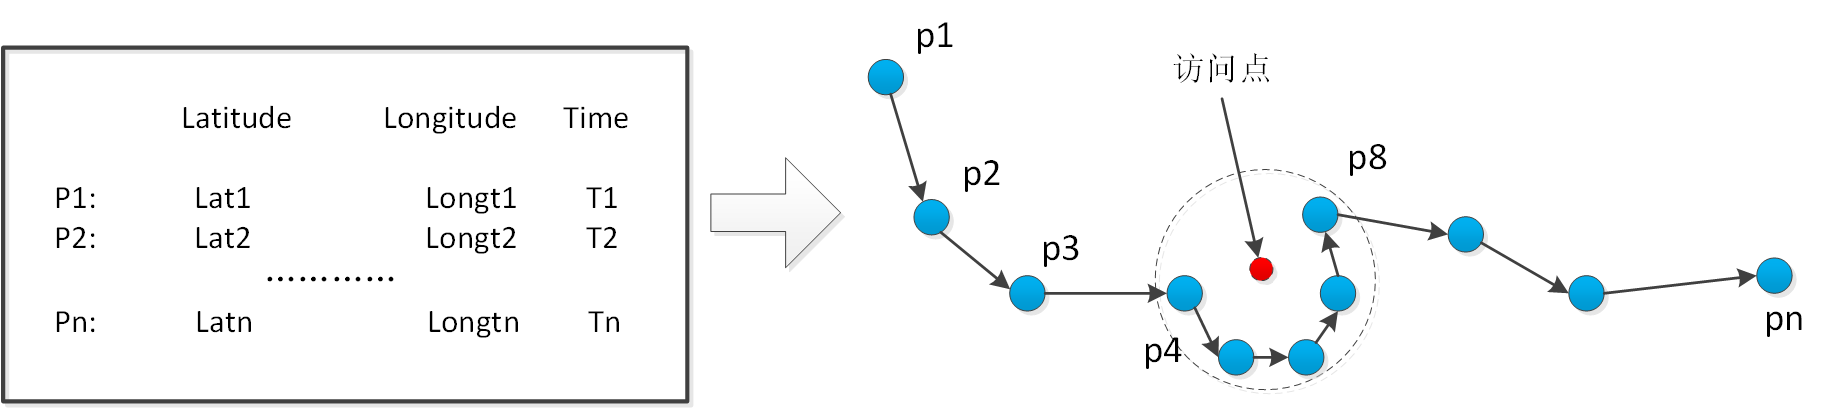
\includegraphics[width=0.8\textwidth]{figure2_1_gps}
\caption{用户GPS轨迹示例图}
\label{fig:2_1}
\end{figure}
\par 停留点的计算过程如\ref{alg2_1staypoint}所示。
\begin{algorithm}[htb]
\caption{停留点检测算法}
\label{alg2_1staypoint}
\begin{algorithmic}[1] %每行显示行号
				\REQUIRE 用户GPS轨迹 $Tra$,$\Delta T$,$\Delta_{distance}$
				\ENSURE 用户停留点序列$SP$
				%\Function {SPDec}{$Tra, \tau_{time},\tau_{distance}$}
				\STATE $i = 0$ , $PointNum= \left| \ Tra \right|$,$SP = Null$
				\WHILE {$i<PointNum$}
				\STATE $j = i+1$
				\WHILE {$j < PointNum$}
				\STATE $distance=Dis(Tra_{i},Tra_{j})$
				\IF {$distance > \Delta_{distance}$}
				\STATE $\Delta_{t}=Tra_{j}.T-Tra_{i}.T$
				\IF {$\Delta_{t} > \tau_{time}  $ }
				\STATE $p.Lat = avg(Tra_{k}.Lat)  $
				\STATE $p.Lng = avg(Tra_{k}.Lng)$
				\STATE $p.T = Tra_{i}.T(arv|lev)$%p.levT = Tra_{j}.T $
				\STATE $SP .add(p) ;j++; $
				\ENDIF				
				\ENDIF				
				\ENDWHILE
				\STATE $i=j ; break$
				\ENDWHILE
				\STATE \RETURN {$SP$}
				%\EndFunction				
\end{algorithmic}
\end{algorithm}
\subsection{聚类算法}
由于现实生活中人们可能会经常多次访问同一个空间地点,但是所计算得到的停留点却可能并不完全相同(坐标的变差,计算的误差等因素影响),因此采用传统直接比较停留点的方法不具备可行性。我们采取对停留点进行聚类的处理方法,这样地理位置非常相近的点就会被划分为同一个类别中。接下来介绍一些常用的聚类算法。
\par 聚类是属于无监督学习中的一种重要的方法,在其他的机器学习方法中如:回归分析、朴素贝叶斯网络等的数据都是带有类别标签$\gamma$,也就是说在训练集中的样例就已经给出了样例的类别,而聚类数据样本却没有给出样本类别$\gamma$聚类的目标是根据组内元素距离最小,组间距离最大将原始数据划分为若干组如图\ref{figure2_1cluster}所示。本节主要介绍几种常用的聚类分析方法:K-Means聚类算法、基于密度的DJ-Cluster 聚类算法以及近年发表的一种改进的基于密度的聚类算法。
\begin{figure}[htp]
\centering
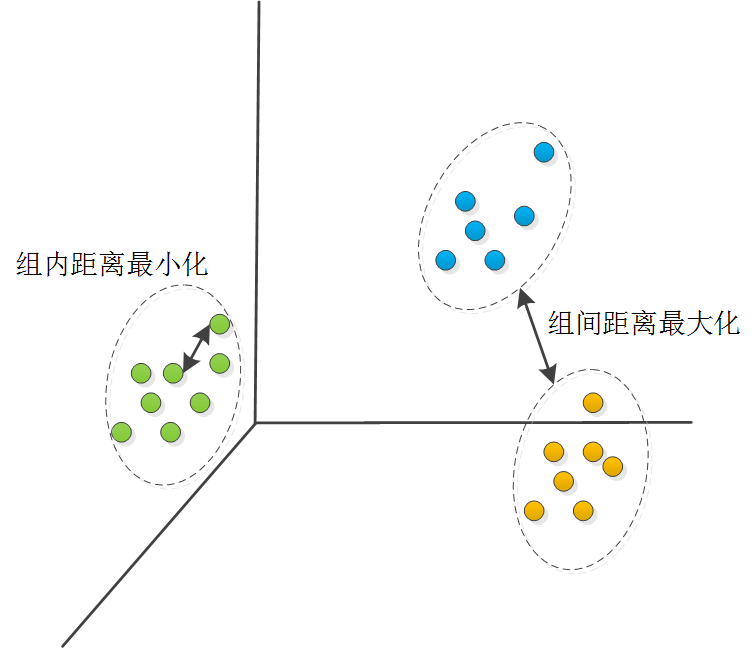
\includegraphics[width=0.8\textwidth]{figure2_1cluster}
\caption{聚类效果示意图}
\label{figure2_1cluster}
\end{figure}
\par  K-means聚类算法是比较经典的聚类方法之一,由J.MacQUEEN在1967提出\upcite{macqueen1967some}。该算法执行效率高,在大规模的数据处理聚类时被广泛使用,该算法输入$k$作为最终聚类的个数,将待分类的$n$个数据分成$k$个簇,使得簇内数据具有高的相似度而簇间的数据存在较低的相似度。K-means聚类算法的执行过程如下:首先根据输入的参数$k$随机从原始数据中选择$k$个对象,每个初始化的对象代表了一个簇的中心;其次,剩余的每个对象计算与簇中心的距离将它们赋予距离最近的簇;第一轮结束后将重新计算每个簇的中心,这个过程不断重复知道准则函数收敛或者簇没有新的变化为止,通常采用平方误差的度量准则如\ref{equ:chap2:k-means}:
\begin{equation}
\label{equ:chap2:k-means}
E=\sum_{i=1}^{k}\sum_{p\subset C}^{p}{\left | p-m_{i} \right |^{2}}
\end{equation}
\par K-means算法虽然简单,易于实现,但是在实际使用过程中需要用户指定$k$的取值,而$k$的取值是难以估计的,针对不同的数据事先并不可能确切的知道这些原始数据应该划分为多少个类别才正确;同时该聚类算法对异常数据非常敏感,一旦出现离群点将容易导致簇中心点出现漂移,对计算结果影响巨大。
%--------写到这里
\par 相比于前面描述的基于距离的聚类方法,研究者于2007年提出了一种基于密度的聚类算法DBSCAN\upcite{ester1996density}以及日后基于该算法改进的DJ-Cluster聚类算法\upcite{zhou2007discovering},DBSCAN算法的基本思想是扫描整个待分类的原始数据集,当扫描到数据对象P 时,计算P的$Eps$邻域内所密度可达的数据对象个数是否大于等于定义的$MinPts$,如果为真,则设立以P为核心的簇,然后尽可能的寻找与该簇密度相连的最大集合或者不断迭代查找该簇中每个数据对象的直接密度可达点,加入到该簇中。如图\ref{fig:figure2_2dbscan}中所示,设$MinPts=3$,从图中我们可以看出原始数据点M,P,O和点R的$Eps$邻域内说包含的点均大于等于$MinPts$因此都可以把它们标记为核心;M是P的直接密度可达,Q是M的直接密度可达。因此可以得知:Q是P的密度可达,但是P不是点Q的密度可达,点O,R和点S是密度相连的。通过实验证明,DBSCAN会受到$Eps$和$MinPts$取值的影响。
\begin{figure}[h]
\centering
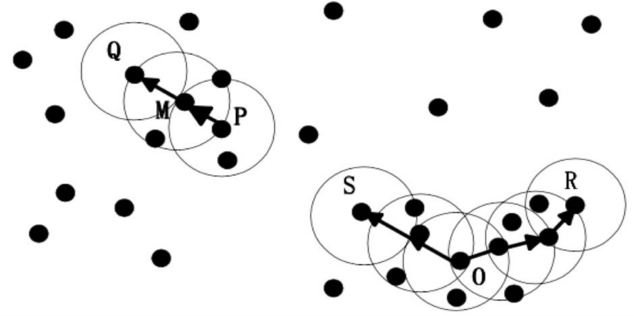
\includegraphics[width=0.8\textwidth]{figure2_2dbscan}
\caption{DBSCAN密度直达和密度可达示意图}
\label{fig:figure2_2dbscan}
\end{figure}
\par Rodriguez A等人2014年在Science上发表了一种新的基于密度的聚类算法\upcite{rodriguez2014clustering}。该算法相比较于之前的聚类算法,具有对参数不敏感便于输出正确的聚类结果的有点。该算法的主要改进想法是针对所有待聚类的组标点基于它们之间的距离,提出了两个新的标准属性:$\rho$和$\delta$,基于聚类中心点具有:中心点自身的密度大,即它的密度超过邻域集合点的密度同时距离其它密度大的中心点之间的距离也足够大这样的特征,其中局部密度$\rho$采用Cut-off kernel计算方式,公式如\ref{equ:chap2:Cut-off-kernel}所示,其中$p_{i}$表示S中与数据点$x_{i}$距离小于$d_{c}$的点的数量;$d_{c}$为截断距离需要用户事先设定并且保证$d_{c} >0$。
\begin{equation}
\label{equ:chap2:Cut-off-kernel}
\rho_{i}=\sum_{j \in I_{s}\setminus {i}}^{ }\chi (d_{ij}-d_{c})
\end{equation}
公式\ref{equ:chap2:Cut-off-kernel}中的$\chi(x)$的计算方式为:
\begin{equation}
\label{equ:chap2:chi-kernel}
\chi{x}=
\begin{cases}
1 & \mbox { $x<0$}\\
0 & \mbox { $x \geq  0$}
\end{cases}
\end{equation}
\par 算法中另一个指标距离$\delta$的定义为设$\left \{  q_{i} \right \}$表示$\left \{  p_{i} \right \}$的降序的下标序列,因此该序列满足:
\begin{equation}
\label{equ:chap2:se-delta}
\rho_{q_{1}} \geq \rho_{q_{2}} \cdots \geq \rho_{q_{N}}
\end{equation}
\par 则可根据公式\ref{equ:chap2:jisuan-delta} 计算出$\delta$:
\begin{equation}
\label{equ:chap2:jisuan-delta}
\chi{x}=
\begin{cases}
\underset{q_{j},j<i}{min} \left \{ d_{q_{i}q_{j}} \right \}  & \mbox { $i \geq 2$}\\
\underset{j\geq 2}{max} \left \{ \delta_{q_{j}} \right \} & \mbox { $i=1$}
\end{cases}
\end{equation}
该算法原理示意见图\ref{fig:2_3}和图\ref{fig:2_4},从图\ref{fig:2_4}可以看出,编号为1和编号为10的坐标点具有较大的$\rho$和$\delta$取值,因此在原始数据中我们将这两个点设置为簇的中心,而在图\ref{fig:2_3}中这两个坐标点恰好是分类簇的中心点;同时还出现了编号26-28三个“离群点”它们的特点是$\delta$值很大而$\rho$取值很小。
\begin{figure}[htp]
\centering
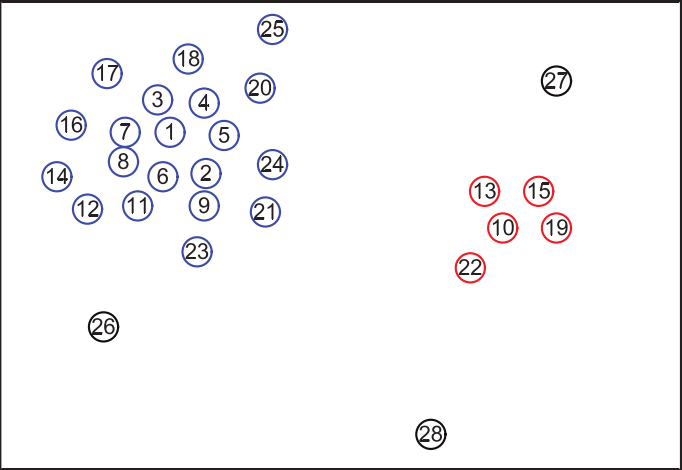
\includegraphics[width=4in]{figure2_3}
\caption{关于decision graph的示例\upcite{rodriguez2014clustering}}
\label{fig:2_3}
\end{figure}
\begin{figure}[htp]
\centering
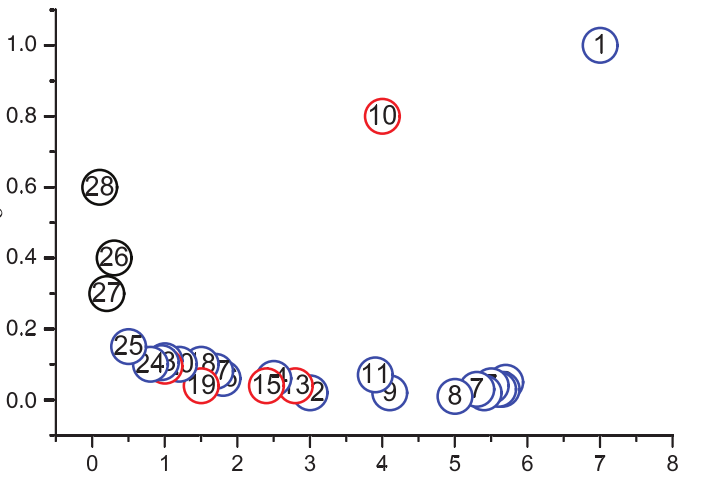
\includegraphics[width=4in]{figure2_4}
\caption{聚类中各点的$\rho$和$\delta$取值\upcite{rodriguez2014clustering}}
\label{fig:2_4}
\end{figure}
\par 总的来说,上述三种聚类算法通过精心调整参数都能取得非常好的聚类效果。不同的算法拥有不同的优缺点,在第四章我们将通过实验来展示各种算法在不同参数下的聚类结果。
\section{时间序列相似度度量方法}
\label{sec:section2-2}
我们阅读了大量社会心理学相关的论文书籍,从中证实得到在现实生活中关系亲密的两个用户会更加倾向于一起进行面对面的交流、共同进行社交活动等,因此通过对手机传感器数据的处理分析能够从中挖掘出人们现实生活中的关系强度。文献[37] 立足于空间距离,提出了在空间距离上非常接近的人们在现实生活中就越可能发生面对面的交互,该文献通过调研一个小区的住户发现人们在现实生活中越是接近,就越容易成为朋友。文献\cite{zajonc1968attitudinal}\cite{zillmann2000mood}进一步通过研究用户的轨迹数据发现由于在空间距离中接近的用户在现实生活中更可能产生交互行为,也就是说拥有相似日常生活轨迹的用户更可能产生交互活动。在现实生活中亦是如此,我们很容易和同自己经常出没同一个地点、行走在同一条轨迹上的人发展友谊关系。
\par 用户的轨迹序列由带有时间戳的位置数据构成,位置数据可能是GPS 也可能是基站号。因此我们可以将轨迹序列看作时间序列,从而使用一些时间序列相似度度量模型来度量轨迹的相似度,下面依次描述编辑距离和DTW这两种相似度度量方法以及序列熵值的计算方法。前面章节描述到用户的轨迹是由GPS位置点所构成的,包含了$(经度,纬度,时间戳)$等详细信息,因此我们将用户的轨迹看作一条由带有时间戳所构成的坐标点序列,采用序列相似度计算方式来处理轨迹之间的相似度。接下来详细描述两种常用的序列相似度计算方法。
\subsection{轨迹中心距离}
传统的计算序列相似度所采用的方法如:编辑距离、汉明距离和夹角余弦等有其优缺点,如果贸然用来计算用户轨迹序列的相似性可能不太符合实际问题的需求,在此基础上,Hechen Liu等学者提出了一种基于用户地理轨迹的相似度度量方法\upcite{liu2012similarity},根据用户的轨迹形状以及时间片内轨迹的中心点之间的距离来作为度量用户轨迹之间相似度的标准。如图\ref{fig:2_3_turn}中(a)图所示,现有两条用户轨迹$Tra_{1}=<a_{1},a_{2},a_{3},a_{4},a_{5}>$和
$Tra_{2}=<b_{1},b_{2},b_{3}>$从观测来看两条轨迹是非常相似的,但是从整条轨迹对比来看,就很难评判两条轨迹是否相似了,因为$Tra_{1}$中有一处急转弯点$a_{3}$,称为转折点。因此算法首先检测出轨迹中的转折点如图\ref{fig:2_3_turn}中(b)再针对每段轨迹中中心点(Center of mass)来计算轨迹之间的相似性。算法中的Center of mass是轨迹$Tra$的质量中心,计算公式如\ref{equ:chap2:Center_of_mass}所示,轨迹计算结果示意图如图\ref{fig:2_3_Center_of_mass}所示,最后再计算轨迹之间的距离,采用余弦相似度来衡量轨迹之间的相似性。
\begin{figure}[htp]
\centering
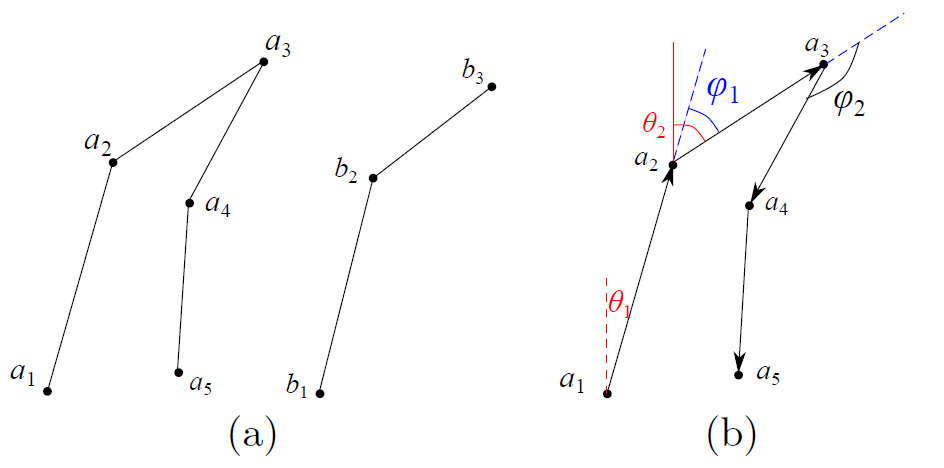
\includegraphics[width=0.8\textwidth]{figure2_1_turnTra}
\caption{轨迹相似计算示例\upcite{liu2012similarity}}
\label{fig:2_3_turn}
\end{figure}
\begin{equation}
\label{equ:chap2:Center_of_mass}
ctr(Tra)=(\bar{x},\bar{y})=(  \frac{\int x f(x)dx  }{\int f(x)dx},\frac{\int y f(y)dy  }{\int f(y)dy} )
\end{equation}
\begin{figure}[htp]
\centering
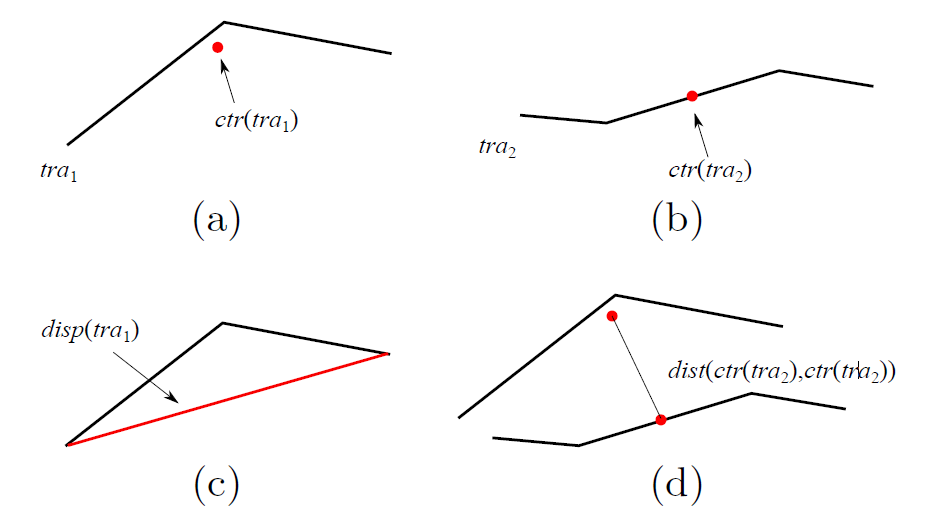
\includegraphics[width=0.8\textwidth]{figure2_1_Center_of_mass}
\caption{基于Center of mass轨迹计算示例\upcite{liu2012similarity}}
\label{fig:2_3_Center_of_mass}
\end{figure}
%-----------------写到这里
\par 采用该算法来计算用户轨迹之间的相似度同直接计算轨迹之间的欧氏距离相比较,能够将轨迹的形状考虑在内,这样能够结合避免直接计算轨迹之间的距离所因为离群点造成了计算结果的巨大偏差。
\subsection{Dynamic Time Warping}
DTW(Dynamic Time Warping)算法最初是由Itakura提出的的一种新型的计算距离的方法\upcite{itakura1987distance},在最初的一段时间是被应用于语音识别领域,在语音识别中即使是同一个词语,由不同的人说出口但是他们的语速、语气等不同造成了单词音频的差别。DTW正由于其计算距离的特殊处理使其能够胜任这一工作。DTW算法采用动态时间规整的思想,将需要比较的两个序列在横轴时间维度上进行压缩、拉伸等操作,使得两条序列具有相同的长度具有更有效的匹配度,同时也消除了传统基于欧式距离计算带来的弊端。
\par 设待计算距离的两个序列,序列$Q$和序列$C$ (两条序列的表示见公式\ref{equ:chap2:dtw_01}、\ref{equ:chap2:dtw_02})。如果两条序列的长度相同,则计算变得很简单。但是如果$m \neq n$,就需要拉伸变形两条序列,使得它们的长度能够尽量对齐同时保留原有序列的信息,算法首先构造一个$n \ast m$矩阵$d$,其中$d[i,j]$ 表示$q_{i}$ 和$c_{j}$之间的距离。采用动态规划的方法来找出序列$Q$和$C$之间的最佳匹配,其中转移方程为找出一条路径使得所有总和的距离$\gamma[i,j]$最小化,具体公式描述见公式\ref{equ:chap2:dtw_03}。
路径及矩阵可视化见图\ref{fig:2_5}。其中:A)为两个待计算比较的序列;B)为通过DTW动态规划求解后两条序列计算距离时所对应的点;C) 将原有序列所对应的位置进行拉伸展开后更加直观的DTW匹配计算结果示意图。
\begin{equation}
\label{equ:chap2:dtw_01}
Q=q_{1},q_{2},…,q_{i},…,q_{n}
\end{equation}
\begin{equation}
\label{equ:chap2:dtw_02}
C=c_{1},c_{2},…,c_{j},…,c_{m}
\end{equation}
\begin{equation}
\label{equ:chap2:dtw_03}
\gamma[i,j]=d[i,j]+min\{\gamma[i-1,j-1],\gamma[i-1,j],\gamma[i,j-1]\}
\end{equation}
\begin{figure}[htb]
  \centering%
  \subfloat[原始序列]{%
    \label{fig:dtw-1}
    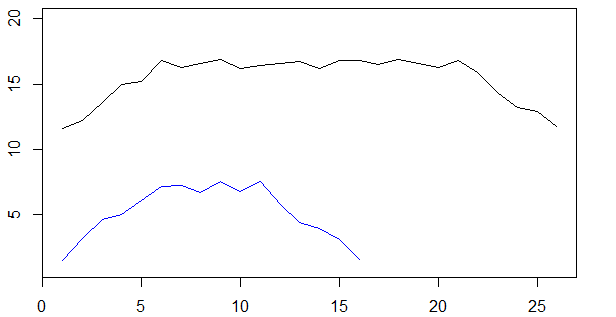
\includegraphics[width=0.4\textwidth]{dtw-1}}\hspace{2em}%
  \subfloat[DTW算法匹配模式结果]{%
    \label{dtw-2}
    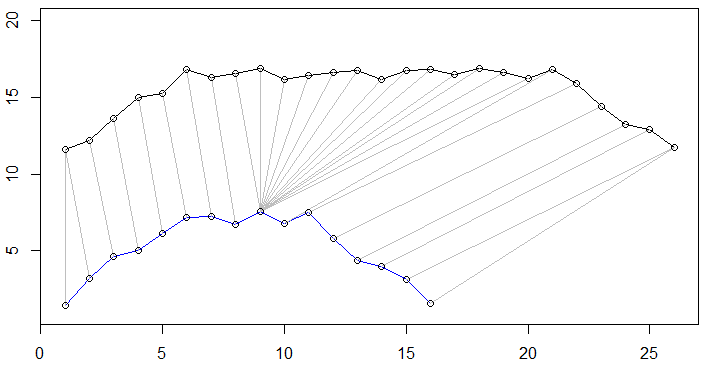
\includegraphics[width=0.4\textwidth]{dtw-2}}\hspace{2em}
    \subfloat[DTW算法拉伸序列计算距离]{%
    \label{dtw-2}
    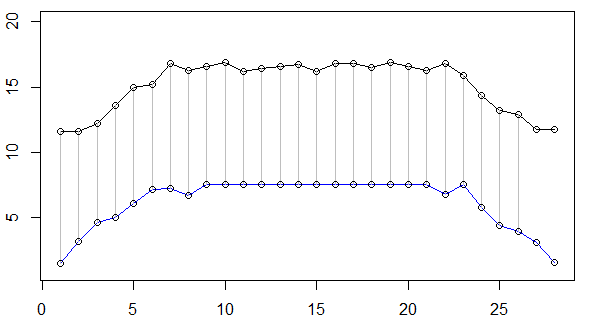
\includegraphics[width=0.4\textwidth]{dtw-3}}
  \caption{DTW算法匹配序列结果示意图}
  \label{fig:2_5}
\end{figure}
\par 通过对DTW算法的原理分析可以得知,序列$Q$和序列$C$的长度越长,则最终计算结果得到的距离就会越大。因此,后者研究中,采用了多种归一化的加权处理方法对结果进行加权处理\cite{ratanamahatana2004everything},获得最优的DTW计算结果。

\section{自然语言处理方法}
\label{sec:section2-3}
相对于用户的空间轨轨迹度量,用户在日常生活中的语义轨迹蕴含了更丰富的上下文信息同时人与人之间在语义轨迹层次上特别是好友之间可能表现出惊人的一致性,如经常去某些地方,在一天中总是先从某个地点出发,再经过某些地点,最后在某个咖啡店相遇等等。基于轨迹的用户模式的交互能够反映出用户在某个空间中的相遇;而基于用户语义轨迹的分析能够在一定程度上展现出用户在社会活动上的相似性,在绪论部分已经详细从社会心理学的研究中描述了人们在现实生活中相遇频率能够反映出用户之间的关系强度,文献\cite{singelis1994measurement}研究发现人们会更加喜欢那些在兴趣、价值观、人格上和自己相似的人。因此通过用户的语义轨迹来在更高的层次上对用户的行为进行相似度计算,进而推测出用户的关系强度。
\par 通过将用户的语义位置序集合同自然语言处理中的文档进行对比, 可以借鉴自然语言处理的算法来处理用户的语义轨迹序列。用户每天的活动轨迹通过语义标签标注后,得到的是一个现实生活中语义轨迹的序列集合,如将一个用户的活动轨迹表示为$<寝室,食堂,教室,图书馆,...,公园>$,通过结合自然语言文档文档相似性计算的思路,把用户每天所计算得到的语义轨迹作为一条原始自然语句,用户在$n$天内所采集的所有轨迹记录就生成了一篇文档,最后基于自然语言处理方法通过计算用户语义轨迹生成的文档之间的相似性来表示用户之间的关系强度。
\par 在以往的研究中,通常使用编辑距离来衡量语句的相似性。在用户轨迹相似分析上,文献\cite{farrahi2008did}借助了LDA主题模型来计算用户语义轨迹之间的相似性,后来的研究在其其基础上对计算方法进行了改进\upcite{yangruosong}。其算法改进在于基于LDA主题模型,将用户的所有语义轨迹看作一篇文档来训练出若干个主题。在计算用户轨迹相似性的时候,将用户用户估计输入到训练好的LDA模型中,然后采用余弦相似度分析比较二者输出的主题分布集合之间的相似度,作为这两个用户之间的关系强度。
\par word2vec是Google在2013年开源的一种词向量计算算法\upcite{mikolov2013efficient}, word2vec借鉴深度学习方法,将文本通过训练的得到文本的$K$维向量表示,通过词与词之间的距离来计算它们之间的相似度。
\subsection{LDA主题模型}
2003年文献\cite{blei2003latent}提出了LDA(Latent Dirichlet Allocation)模型对自然语言进行建模,可以用来识别文档语料中潜在的主题信息。整个计算模型采用了词袋的计算方法,计算出文档的向量表示,每一篇文档计算出一部分主题的概率分布,而每一个主题内又可以表示为很多词语的一个概率分布,LDA的训练过程为:遍历每一个文档,在主题分布袋中随机抽取一个主题;然后在被随机抽取到的主题中再随机抽取一个单词;最后重复上述步骤直到遍历完文档中的所有词语。整个生成的过程可以用图\ref{fig:2_6}表示:对于每一份文档与设定的$T$个主题之间的概率分布对应$\theta $,每个主题与词袋中的$V$个词语之间的概率分布$\phi$,其中$\theta $和$\phi$分别有一个参数$\alpha$和$\beta$的狄利克雷的先验分布,这样对于任意一份文档$d$中的每一词语,我们从与文档相对应的概率分布$\theta $中选取一个主题$z$,随即在根据与主题$z$对应的概率分布$\phi$中选取一个词语$w$,最后重复上述过程$N_{d}$次,就能够产生文档$d$,公式\ref{equ:chap2:lda_01}为LDA的核心公式。
\begin{figure}[htp]
\centering
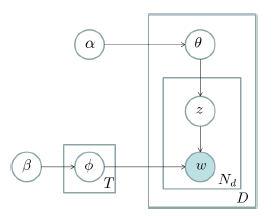
\includegraphics[width=0.6\textwidth]{figure2_6_lda}
\caption{LDA的图模型表示}
\label{fig:2_6}
\end{figure}
\begin{equation}
\label{equ:chap2:lda_01}
p(w|d)=p(w|t) \ast p(t|d)
\end{equation}
% 写到了这里------------------
\subsection{word2vec}
word2vec是Google在2013年开源的一种词向量计算算法\upcite{mikolov2013efficient}, word2vec借鉴深度学习方法,将文本通过训练的得到文本的$K$维向量表示,也就是说把特征转换到了$K$维空间进行表示,通过词与词之间的距离来计算它们之间的相似度。word2vec采用了三层的神经网络结构即为输入层-隐含层-输出层构成,其主要方法是借助哈夫曼编码针对相似词频的词语构建出相似的隐藏层激活函数,算法采用了层次化的Log-Bilinear模型,其中一种是基于CBOW(Continuous Bag-of-Words Model)的计算模型,在CBOW模型中,根据上下文信息可以预测下一个词语$w_{t}$,其公式如\ref{equ:chap2:word2vec_01}所示,CBOW的计算模型如图\ref{fig:2_7_cdow}所示。
\begin{equation}
\label{equ:chap2:word2vec_01}
p(w_{t}|context)=p(w_{t}|w_{t-k},w_{t-k+1},\cdots ,w_{t-1},w_{t+1},\cdots w_{t+k})
\end{equation}
\par 现在的CBOW计算采用层次的Softmax算法,每个单词$w_{i}$都可以有一条从根节点出发被唯一访问到的路径,这条路径就形成了词语的编码。
\begin{figure}[htp]
\centering
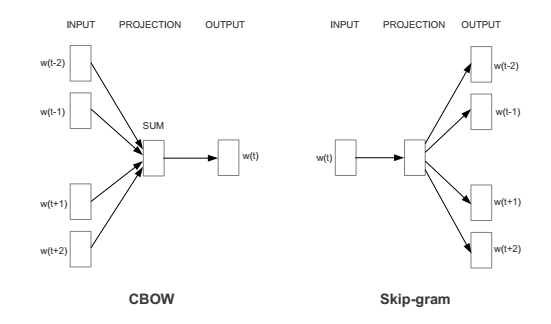
\includegraphics[width=0.8\textwidth]{figure2_7_cdow}
\caption{word2vec神经网络结构图\upcite{mikolov2013efficient}}
\label{fig:2_7_cdow}
\end{figure}
\begin{figure}[htp]
\centering
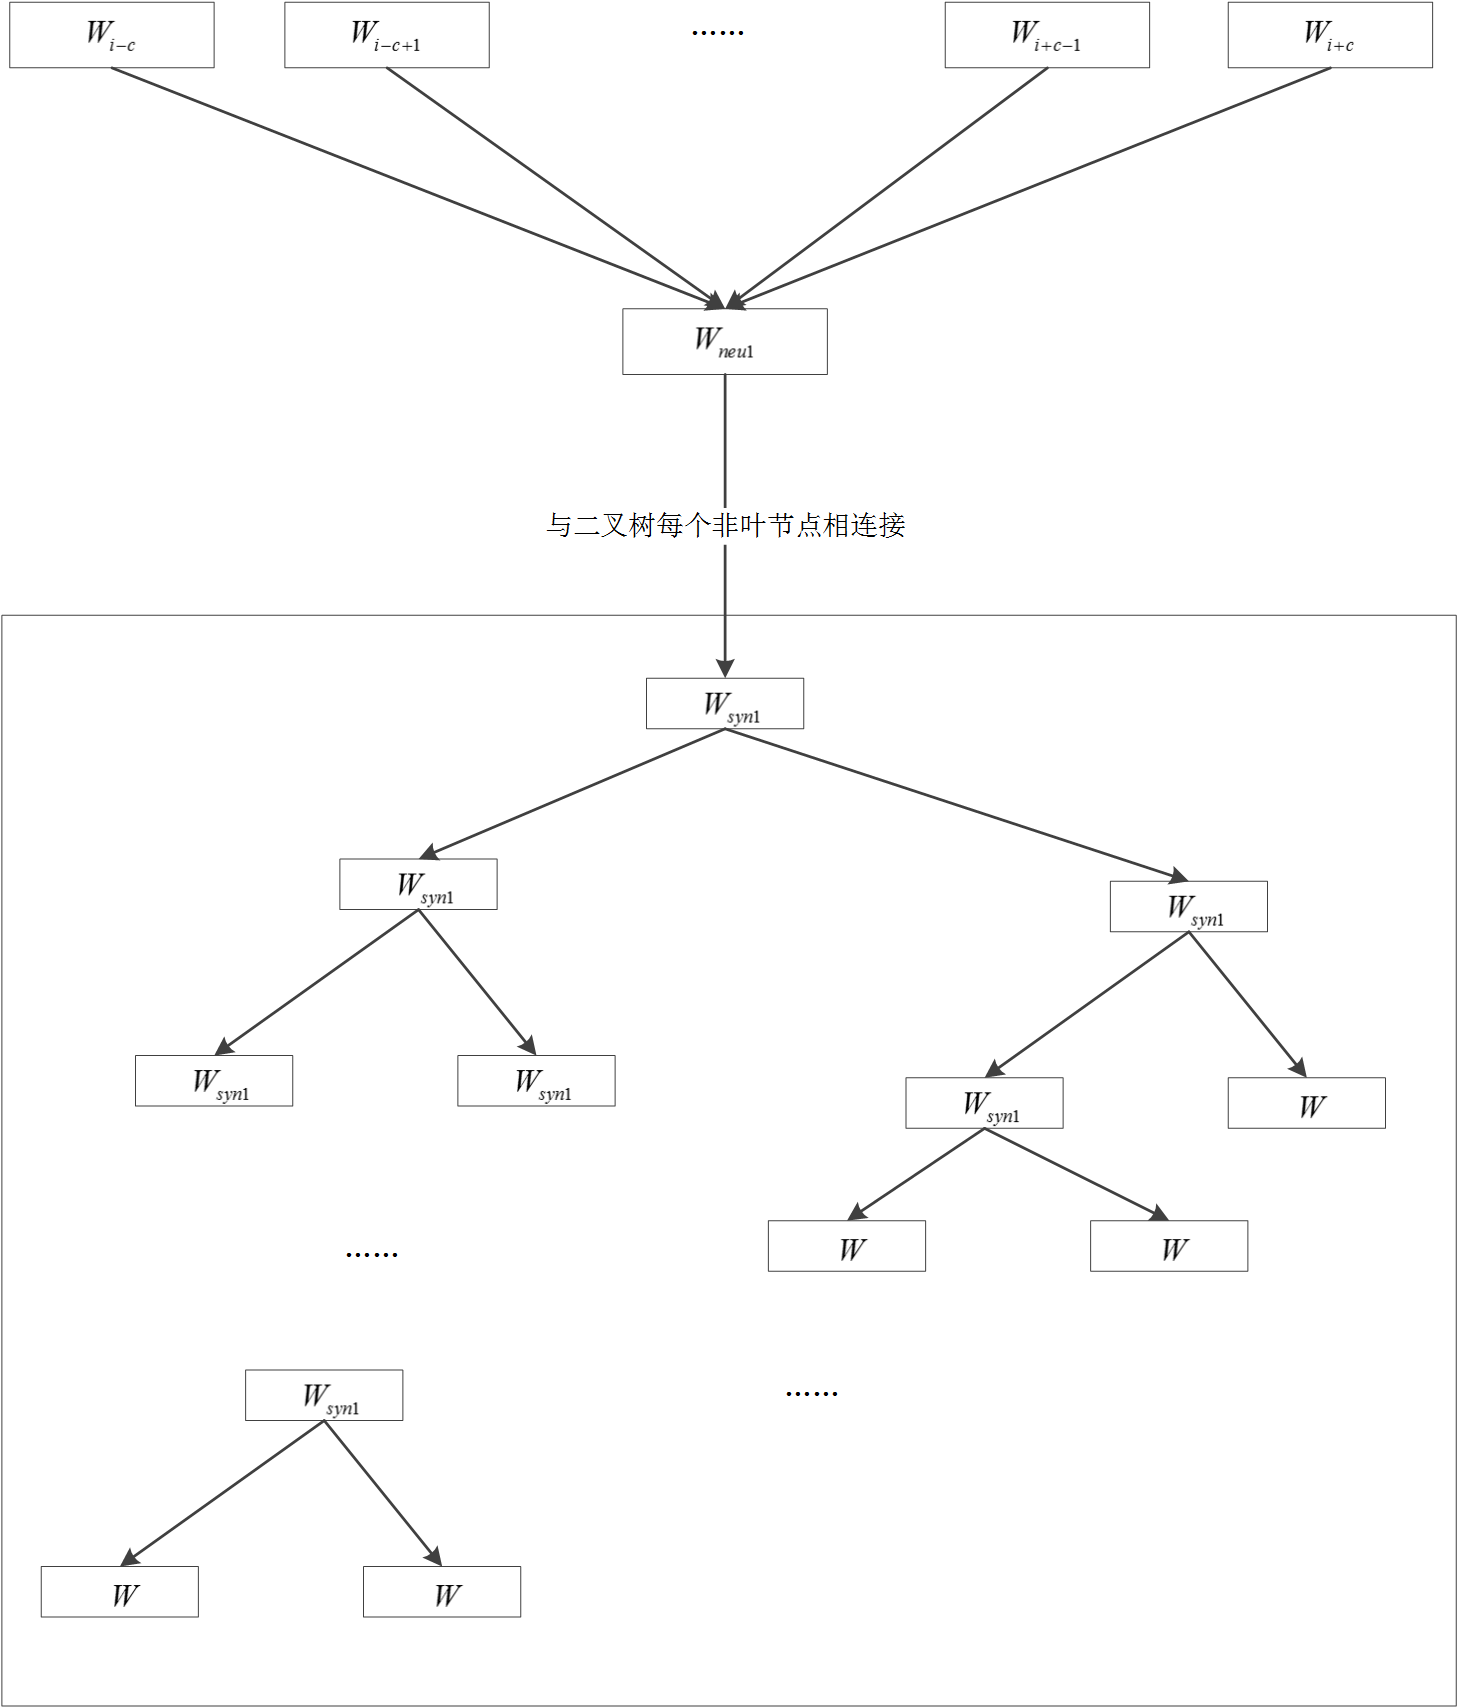
\includegraphics[width=0.7\textwidth]{figure2_7_w2cmodel}
\caption{word2vec神经网络结构图}
\label{fig:2_7}
\end{figure}
\par 在图\ref{fig:2_7}中,第一层也称之为输入层, 它的输入是词向量;中间的层次为隐含层,得到的的输入是输入层若干个词向量的向量累加结果;第三层则是由二叉树所构成的霍夫曼树所组成的输出层,其中每个非叶节点是一个计算后的向量但是不同于输入层的词向量,这里计算后的向量不代表某个词语,而是表示一个类别的词语,同时这棵霍夫曼树的所有叶子节点包含了输入词袋中的所有词。
\par 对于词袋$BG$中的单词$w$,在图\ref{fig:2_7}中一定能够找到有且仅有一条从Root节点到叶子节点$w$的路径。路径中的每一次分支都是一个概率问题,因此得到\ref{equ:chap2:word2vec_01}中的数学表达式,将其中的$w_{i}$用词向量替换,得到该三层神经网络的目标公式如\ref{equ:chap2:w2v_03}, $Num^{w}$表示从Root节点到词向量节点$w$路径中包含的节点个数,$w_{j}$表示该路径上的第$j$个词,$v_{w}$表示词$w$对应的词向量,$\sigma$表示SIGMOID函数,通过求解目标函数的最大值,就可以得到每个词所对应的向量。
\begin{equation}
\label{equ:chap2:w2v_03}
L=\sum_{w\in C}\sum_{j=2}^{Num^{w}}\{(1-w_{j})log[\sigma(v_{w}^{T}\theta_{j-1}^{w})]+w_{j}log[1-\sigma(v_{w}^{T}\theta_{j-1}^{w})]\}
\end{equation}
\subsection{快速Hash算法}
基于word2vec的计算方法针对文档的分词结果,再根据神经网络模型计算得到每个词的向量表示,但是这样无疑增加了整个计算过程的时间复杂度,本文研究目的是能够为众多用户提供一种计算关系强度的框架,因此如果采用传统的Hash算法进行处理,则能够减少程序的运行时间,来自于GoogleMoses Charikar针对海量文档快速计算相似计算提出了一种局部敏感hash算法\upcite{manku2007detecting},其核心内容恰巧和word2vec相反:希望将数据进行降维处理,将原始的高维词向量通过一系列运算映射到低维的词向量,最后来计算相似性。
\par 以上介绍了几种方法在自然语言处理中都得到了广泛的应用,因此综合考虑使用最后一种方法来作为计算方法, 在后面还会详细讲解如何使用hash来度量用户之间的关系强度,以及在不同处理方法之间进行横向和纵向的比较。
\section{WiFi和蓝牙数据的度量方法}
WiFi和蓝牙作为一种主动对外界感知和探索所得到的感知信息,已经证实能够被用来分析用户之间的社交关系。文献\cite{hsu2007mining}通过收集到用户的WiFi数据,然后将用户的WiFi数据同现实语义位置进行关联,得到了WiFi的语义向量,这样就能够得到基于WiFi的用户活动轨迹序列,提出了一种新的模型AMVD(average minimum vector distance)来计算人与人之间的距离,其计算公式如\ref{equ:chap2:amvd}所示,其中$a_{i}$和$b_{j}$表示用户A和用户B之间的联合向量,$d(a_{i},b_{j})$表示计算二者向量之间的曼哈顿距离。
\begin{equation}
\label{equ:chap2:amvd}
AMVD(A,B)=\frac{1}{\left | A \right |}\sum_{\forall a_{i} \in A}^{ }  \mathop{\arg\min}_{\forall b_{j} \in B} d(a_{i},b_{j})
\end{equation}
\par 蓝牙数据和GPS轨迹数据都能够推测出用户之间的交互行为,蓝牙作为一种近距离的无线通讯手段,收到波长影响使得通讯距离只能是5-10米内,因此蓝牙感知数据能够进一步描述了用户之间在现实生活中的物理接触。前人的研究中,有根据蓝牙信息来简单计算出用户在现实空间中的面对面交互次数,从而推测出用户的社会关系情况\upcite{eagle2009inferring,zheng2013unsupervised}。在本文中,我们使用了新的数据结构来表示用户的WiFi、蓝牙感知数据,同时直接计算其感知上下文环境信息的相似度作为用户之间环境的相似度的参照。
\section{小结}
\label{sec:section2-4}
本章详细的从本课题研究的三个数据源出发对不同数据源的研究方法、现状进行了详细的分析和讨论。2.1节讨论了在用户原始GPS轨迹数据处理中要解决的三个主要问题:剔除异常点、停留点检测以及空间轨迹的聚类。2.2节则是介绍了计算用户轨迹序列相似度的常用方法,并以此结果作为用户的关系强度计算结果。2.3节从自然语言处理的角度介绍了常用的文档相似性检测计算方法,为计算用户语义轨迹的相似度提供了可行性算法。2.4节从WiFi和蓝牙数据处理计算角度出发,介绍了前人研究的计算方法理论,为本研究中所采取的基于上下文环境的计算方式作出铺垫。
\chapter{RSMHD用户关系强度计算框架模型}
\label{chap:chapter07}
上一章详细介绍了和本研究数据源相关的处理技术与方法,接下来这一章将主要介绍RSMHD的多维据源多维度的关系度量模型的整体框架结构。
\section{RSMHD模型框架描述}
\label{sec:section7-1}
本研究的主要内容是通过采集到的用户感知数据(GPS轨迹信息 、WiFi数据、蓝牙数据)来开展用户之间的关系强度度量工作。因此本文希望能够提供一种基于此类非社交的感知数据建立的通用的用户关系强度计算框架。非社交数据主要是指不是来自于用户直接社交活动中所收集到的数据,在本研究中主要包含了用户轨迹数据、用户WiFi感知数据和用户蓝牙感知数据。因此本课题基于以上三种不同的感知数据源提出了能够统一处理多种数据源的计算框架,其整体概要结构图如图\ref{fig:7_1}所示,图中描述整体架构由以下几部分组成:上下文感知收集模块、基于用户日常轨迹的关系强度计算模块、基于用户WiFi感知数据的关系强度计算模块和基于用户蓝牙的关系强度计算模块。用户的日常语义轨迹是有连续的GPS位置点所组成的轨迹的集合,在用户的轨迹信息的采集过程中,因受到地形、气候、GPS 传感器的干扰误差的影响,会出现GPS漂移现象,GPS的位置漂移使得用户的轨迹数据中存在大量的噪音数据,影响后续对数据的处理和分析。因此对采集到的用户轨迹数据采取滤波处理,消除轨迹中所蕴含的噪音数据。GPS 位置的采集还受到地形环境的影响,在室内无法获取GPS 位置信息的时候会导致用户轨迹的缺失,造成计算结果产生巨大偏差。第四章部分将重点针对上述问题展开GPS轨迹的处理研究工作,以获得好的信息效果。对于剩余的WiFi和蓝牙感知数据来讲,主要的工作是针对二者数据源的特点以及后续的算法输入对原始数据进行提取和结构化建模表示存储。第四章的其余部分将会针对WiFi和蓝牙感知数据的预处理和结构化表示进行详细的描述。
\begin{figure}[htp]
\centering
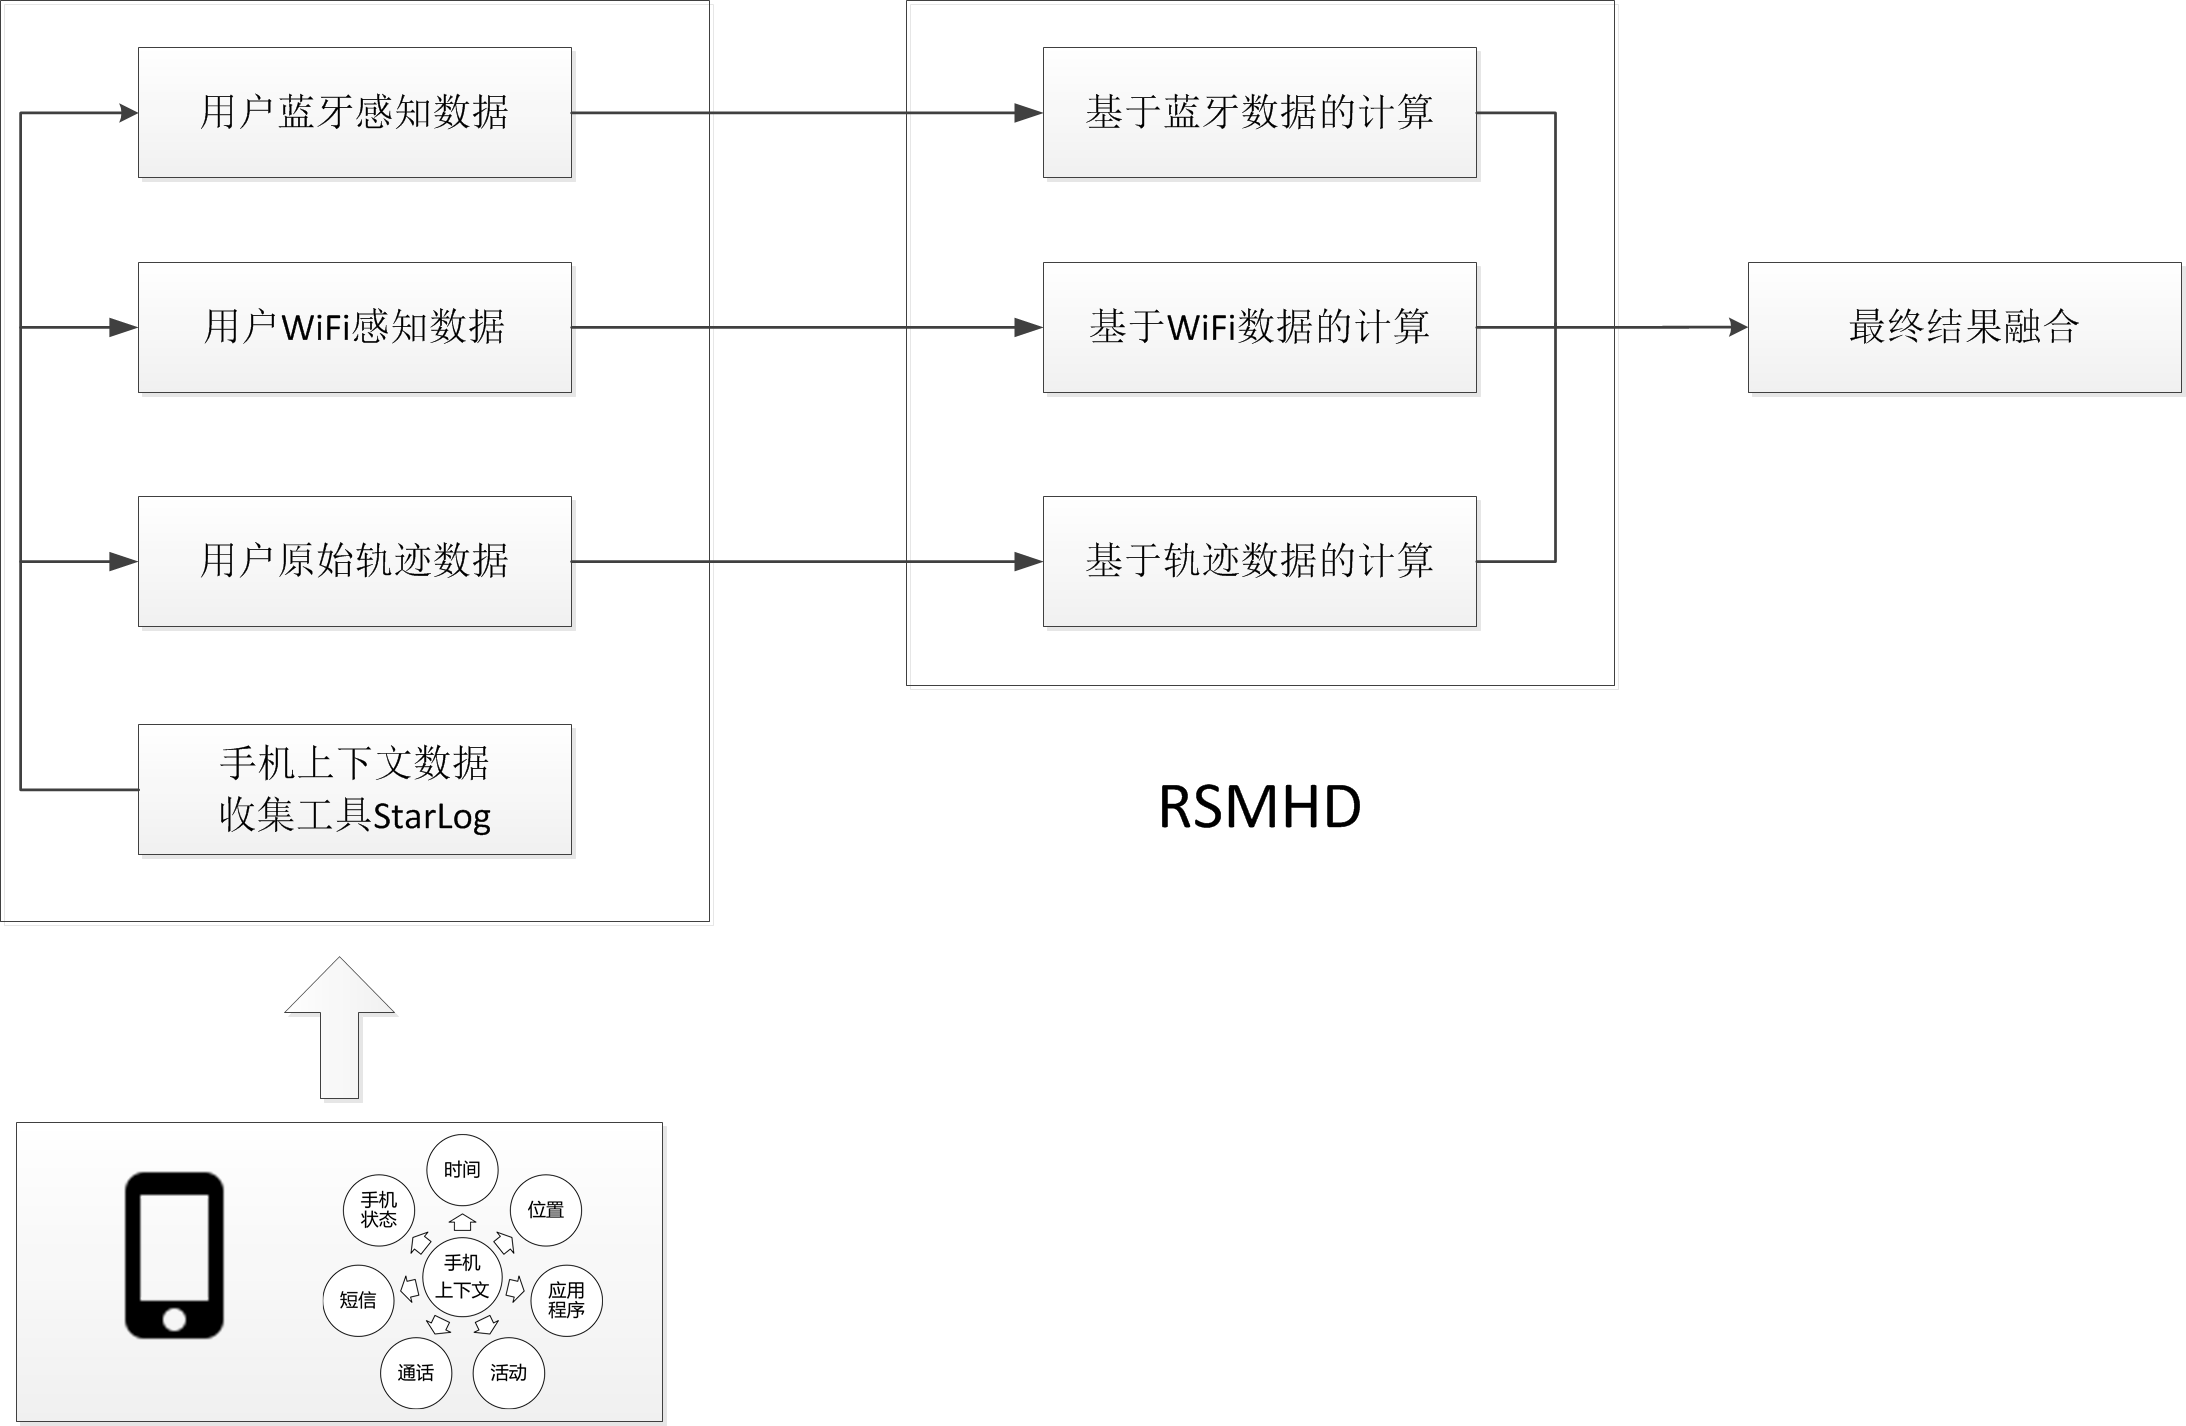
\includegraphics[width=0.8\textwidth]{figure7_1_RSMHD}
\caption{RSMHD用户关系强度计算模型框架图}
\label{fig:7_1}
\end{figure}
\subsection{基于轨迹数据的关系强度计算模块概述}
在本研究中所提出的RSMHD计算框架模型中,第二层需要基于用户的日常语义轨迹分别通过计算地理轨迹相似性、用户的语义轨迹相似性以及日常轨迹运动模式三个层次关系强度融合为轨迹强度结算结果,其详细框架图如图\ref{fig:7_1_tra}所示。在这个模块中,通过计算用户日常地理轨迹的相似性推测出用户之间的关系强度;针对用户活动产生的日常语义轨迹,RSMHD 模型采利用自然语言处理的思想,通过快速编码变换计算出用户基于语义轨迹的关系强度;第三层中,RSMHD 进一步挖掘出用户轨迹中更高一层的上下文信息(High Context)得出用户日常轨迹模式如:用户A 经常喜欢到校外某地用餐、用户B 经常下午在操场跑步等这些代表用户日常轨迹活动模式的信息,计算用户之间基于运动模式的关系强度。
\begin{figure}[htp]
\centering
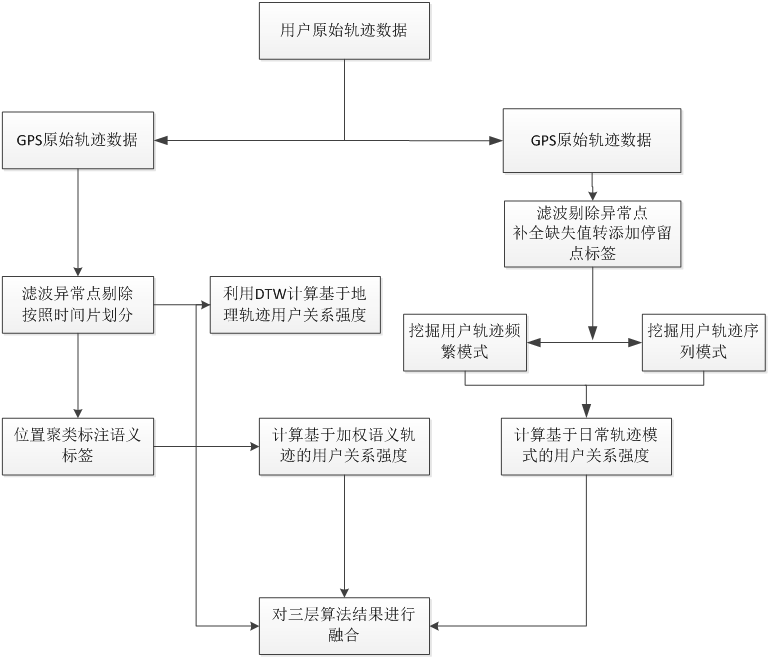
\includegraphics[width=0.8\textwidth]{figure7_1_tra}
\caption{RSMHD中基于用户轨迹计算模块详细框架图}
\label{fig:7_1_tra}
\end{figure}
\subsection{基于WiFi和蓝牙数据的关系强度计算模块概述}
在RSMHD计算框架模型中我们针对WiFi和蓝牙原始数据的特点以及现实生活中WiFi和蓝牙上下文环境的特征,采用了区别于原有基于WiFi和蓝牙计算社交关系的方法,整体的详细计算框架如图\ref{fig:7_1_wifi}所示。在WiFi和蓝牙数据处理计算框架中,分别针对底层手机的上下文感知信息进行数据信息的提取的规整,从复杂冗余的信息中萃取出关键的富有价值的信息;然后结合WiFi和蓝牙各自的上下文环境特征信息,将整理后的数据用图的数据结构进行结构化表示,使得抽象表示后的数据结构更加符合现实中的含义;最后基于结构化后的感知数据进行关系强度计算,将结果输出到下一层。
\begin{figure}[htp]
\centering
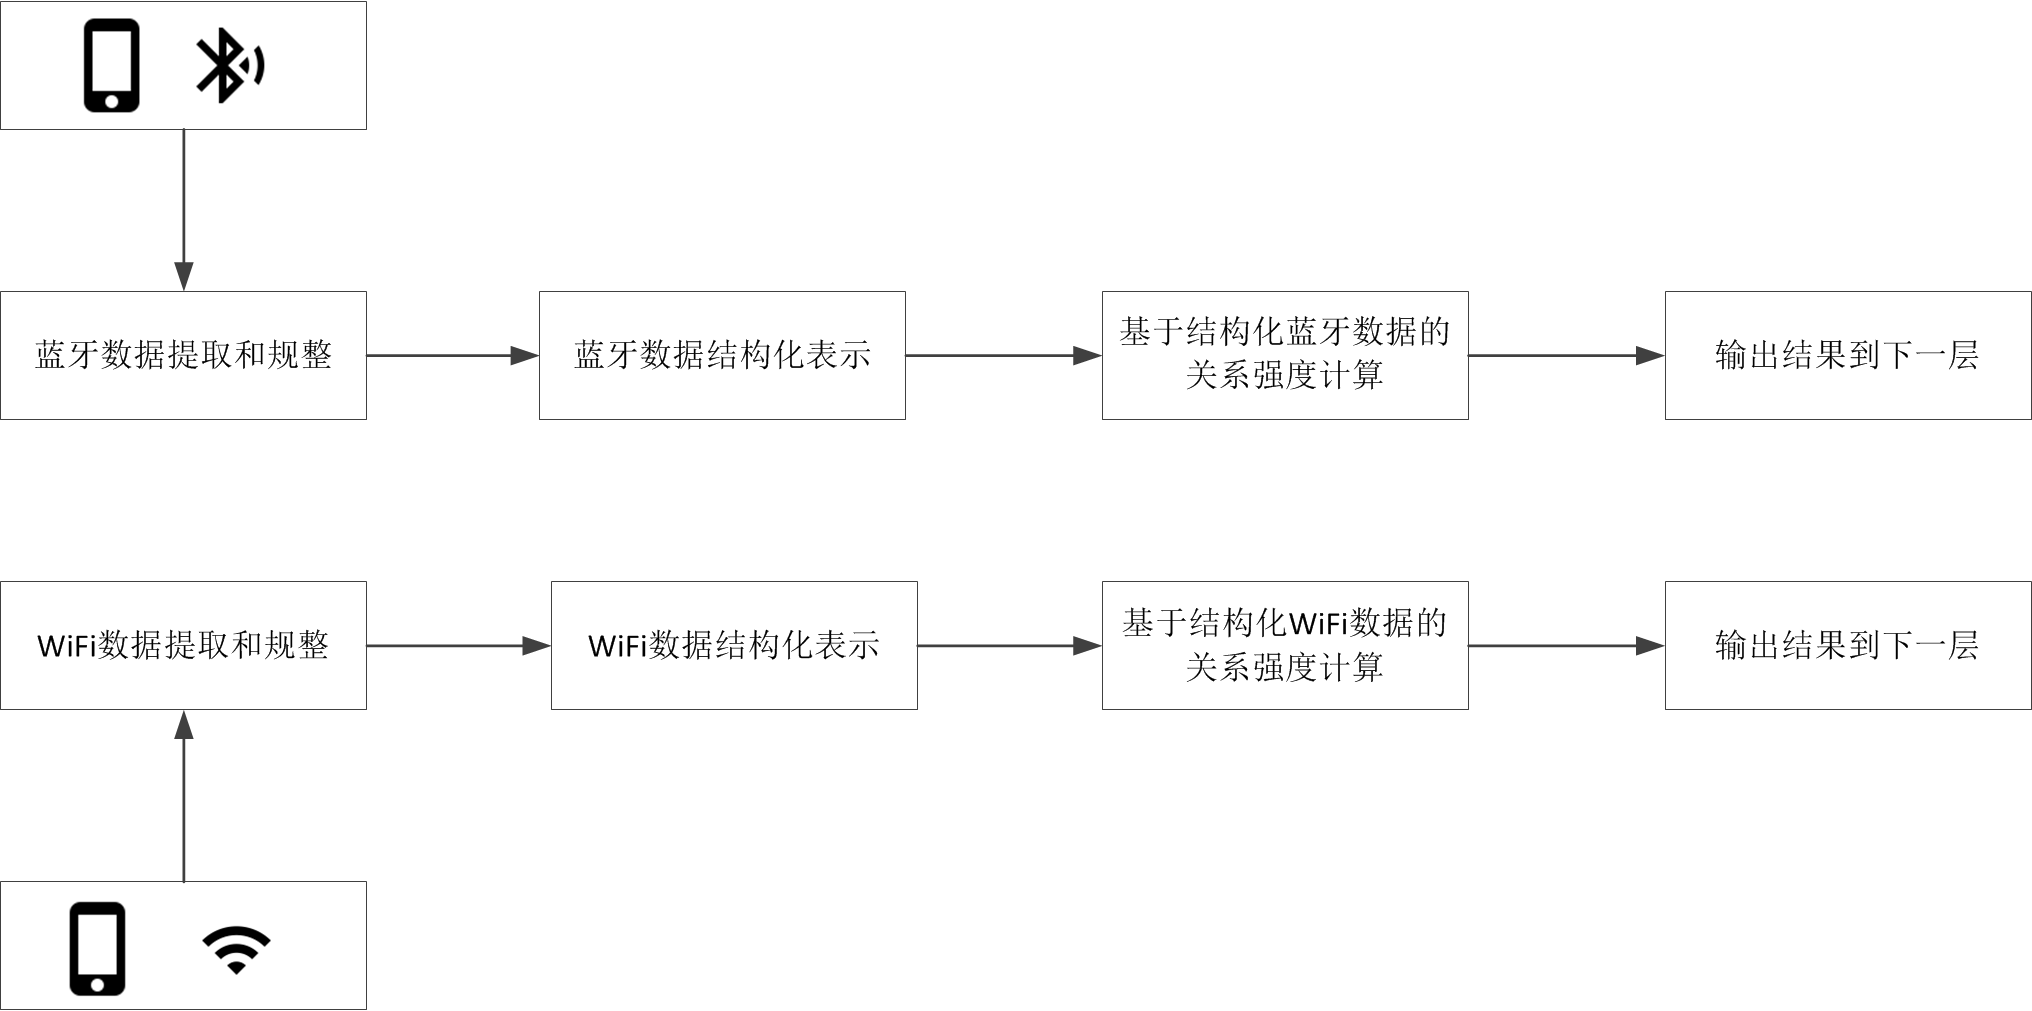
\includegraphics[width=0.8\textwidth]{figure_3_RSMHDwifibluee}
\caption{RSMHD中基于WiFi和蓝牙计算模块详细框架图}
\label{fig:7_1_wifi}
\end{figure}
\section{RSMHD模型计算流程概述}
\label{sec:section7-2}
整个信息采集是采用我们自己编写的用户手机上下文信息收集工具StarLog来记录保存用户手机的上下文感知数据如:GPS位置信息、WiFi感知信息、蓝牙感知信息、脱敏的通话记录、短信记录、APP使用记录等。
\par 针对用户的GPS位置数据我们首先对轨迹数据进行预处理,即采用滤波算法检测出用户日常轨迹中的漂移点减少轨迹中的噪音;然后根据停留点检测算法识别出用户轨迹中的停留点,针对缺失的轨迹点进行预测补全;第一层次中针对用户日常空间轨迹相似性计算时,可用将每天的轨迹数据划分为若干时间片的数据,然后采用DTW加权算法对时间片内的空间轨迹相似度进行计算并按照一天的轨迹进行处理。对于基于用户语义轨迹推倒关系强度这层我们首先将得到的停留点进行聚类分析,得到聚类后的停留点集合因此对于每一个簇都是同一个语义位置,然后将聚类GPS转换为现实社会中的语义标签,在计算用户语义轨迹的相似性时,采用快速hash算法将用户分片后的语义轨迹序列作为输入,得到用户之间每天的语义轨迹相似度,以及最终的语义轨迹相似度并将结果作为用户自己的关系强度。在上一层的基础上,我们针对得到的用户语义估计进行挖掘,寻找出用户的日常运动模式,然后计算用户运动模式之间的相似度并作为关系强度之一进行输出,综合三层的计算结果得到用户基于轨迹数据计算得到的关系强度。
\par 其次针对用户的WiFi和蓝牙数据,首先从原始数据中提取出重要的信息,并将WiFi和蓝牙数据进行结构化存储处理,采用图的存储结构,将WiFi和蓝牙数据还原为现实生活中的存在环境,然后针对用户切片时间内每刻的感知环境进行相似度计算,并将一天中的计算结果进行汇总进一步得到所有时间段内的用户相似度,最后将结果作为基于两种数据源推测出的用户关系强度。
\par 最后,在基于前面三种数据源的用户关系强度计算结果的基础上,采用集成学习的思想对计算结果进行融合处理,得到最终的用户关系强度计算结果。

\chapter{RSMHD框架的相关技术研究}
\label{chap:chapter03}
上一章节主要是对本课题研究的RSMHD框架进行了详细的描述,本章接下来将针对每一个模块中的具体面对的问题以及采取的方法进行详细描述,包括噪音点的剔除、如何语义轨迹、如何计算轨迹相似性以及如何对WiFi和蓝牙数据进行结构化处理等。
\section{GPS轨迹处理计算技术}
\label{sec:section3-1}
用户的日常GPS轨迹数据包含了用户的生活工作以及娱乐等丰富的上下文信息,如图\ref{fig:tramodel}所示,我们基于用户的日常轨迹分别从地理位置相似性、语义轨迹相似性以及轨迹模式相似性出发度量人与人之间的关系强度。模块的输入是由StarLog收集的GPS感知数据,通过对初始数据的解析提取得到原始的GPS位置点构成的用户轨迹序列。预处理阶段主要是通过滤波算法对原始轨迹序列进行异常点检测,并通过轨迹预测补全缺失的部分GPS轨迹序列;第二层中将第一层得到的停留点赋予语义得到用户的语义轨迹序列,采用自然语义处理思想计算基于语义轨迹的相似性;再往上一层,从用户的历史轨迹数据中挖掘出的频繁模式和序列模式能够反映出用户的日常轨迹运动习惯和行为规律,运动模式在现实生活中表现为用户经常行走的路径序列,是用户轨迹数据规律的抽象表示,最后计算用户之间的关系强度。
\begin{figure}[htp]
\centering
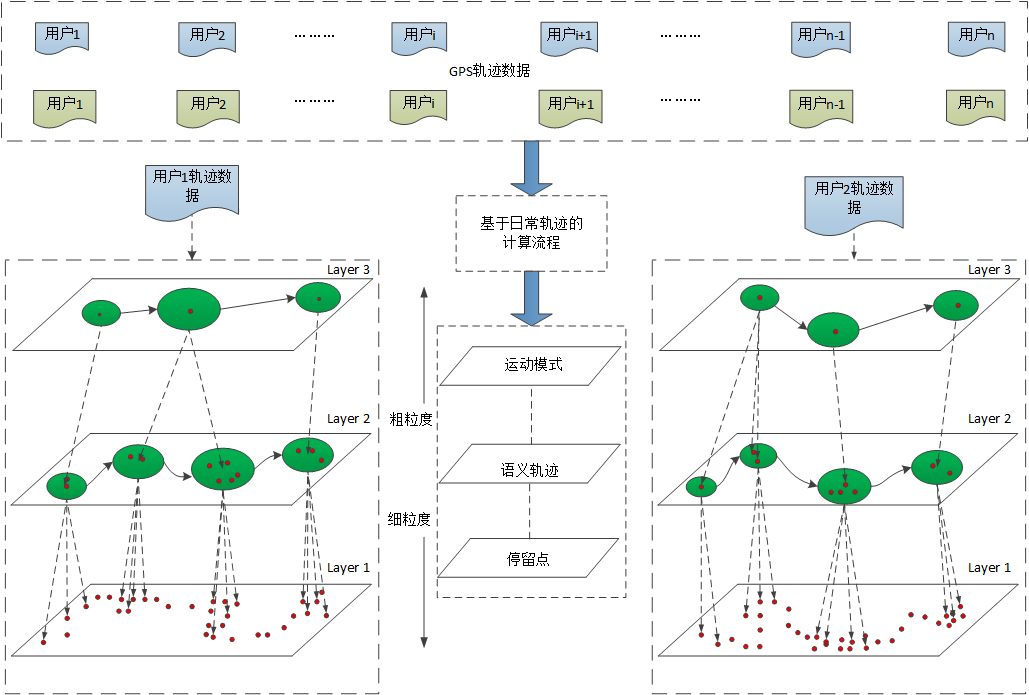
\includegraphics[width=0.8\textwidth]{figure4_2}
\caption{基于多层次多粒度轨迹的用户关系强度计算}
\label{fig:tramodel}
\end{figure}
\section{GPS轨迹预处理与语义化}
\label{sec:section3-2}
本节主要讲述如何对GPS轨迹数据进行清洗规整,以及得到用户的语义轨迹进行结构化存储。
\subsection{剔除轨迹中的异常点}
前文已经提到,由于在获取GPS位置信息的时候会受到位置漂移的影响,导致在获取用户实际位置的时候可能产生采样的误差甚至跳跃,为了使得最终计算得到的关系强度结果更为准确我们需要对GPS轨迹数据进行滤波分析。在第二章中描述了常用的三种滤波方法,在本章中将会针对三种滤波算法进行最后结果展示并根据结果分析最终采用此滤波算法的原因。
\par 首先接下来使用我们自己开发的用户感知数据收集软件StarLog,来分析观察各种滤波算法对用户轨迹中异常点检测剔除的效果,如图如图\ref{fig:3_2_1}、\ref{fig:3_2_2}所示。
\begin{figure}[htb]
  \centering%
  \subfloat[原始轨迹数据]{%
    \label{fig:3_2_1_1}
    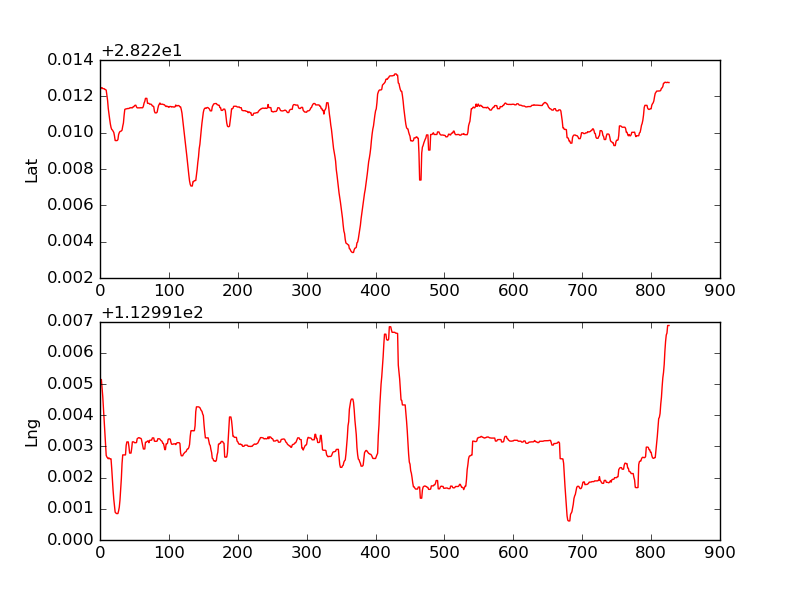
\includegraphics[height=4cm]{figure_4_mid_location1}}\hspace{4em}%
  \subfloat[中值滤波后的轨迹数据]{%
    \label{fig:3_2_2_1}
    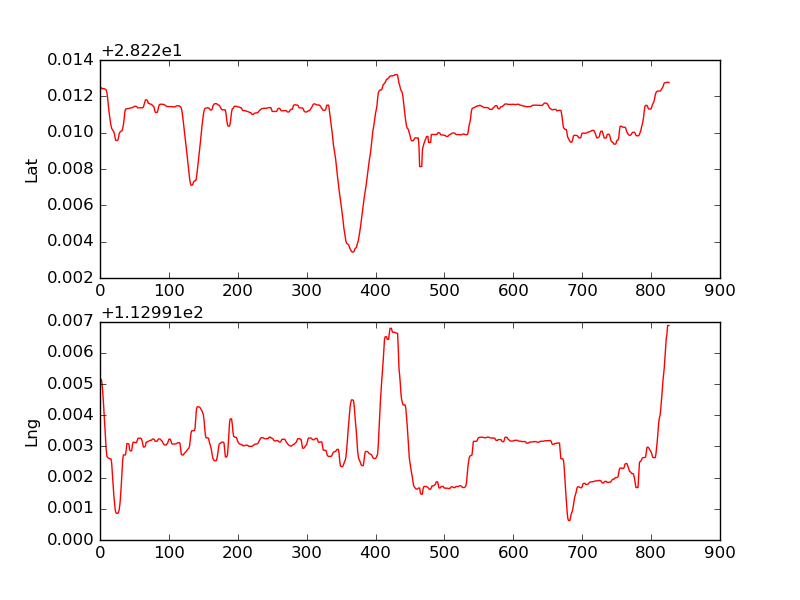
\includegraphics[height=4cm]{figure_4_mid_location1_ed}}
  \caption{轨迹中值滤波实验结果1}
  \label{fig:3_2_1}
\end{figure}
\begin{figure}[htb]
  \centering%
  \subfloat[原始轨迹数据]{%
    \label{fig:3_2_2_1}
    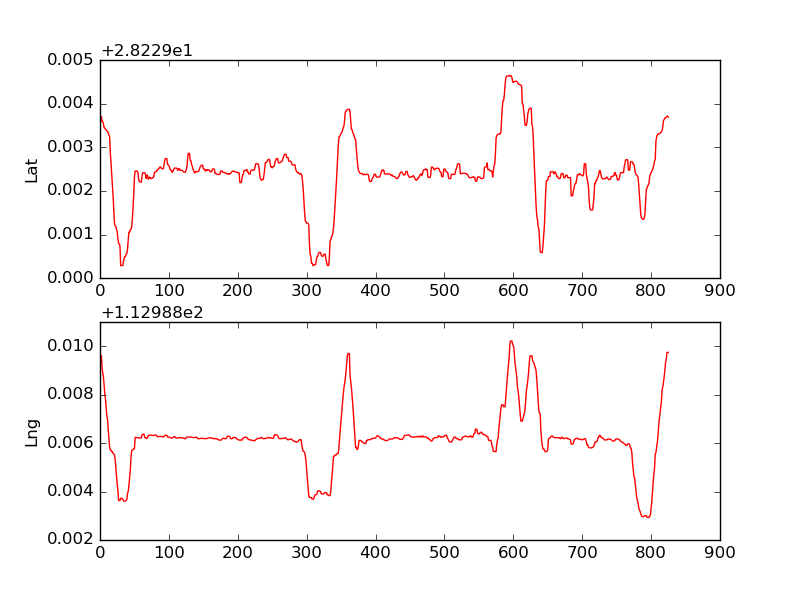
\includegraphics[height=4cm]{figure_4_mid_location2}}\hspace{4em}%
  \subfloat[中值滤波后的轨迹数据]{%
    \label{fig:3_2_2_2}
    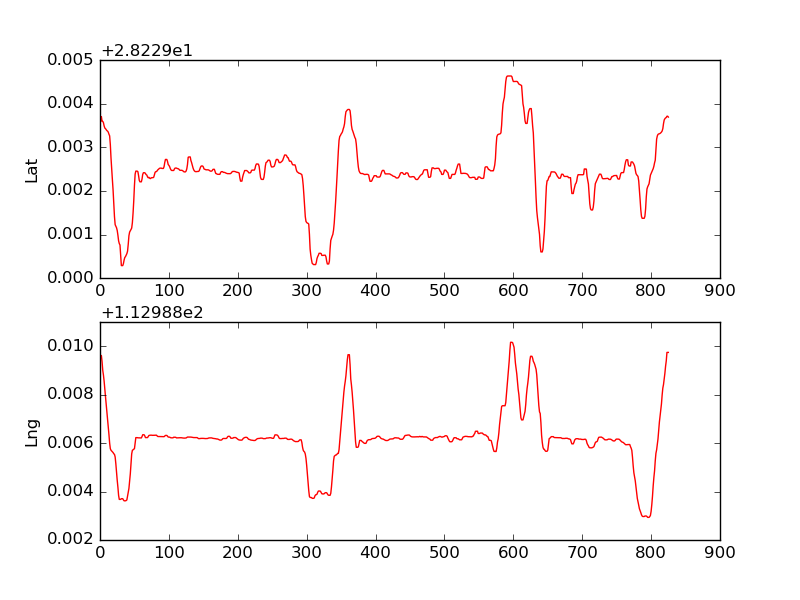
\includegraphics[height=4cm]{figure_4_mid_location2_ed}}
  \caption{轨迹中值滤波实验结果2}
  \label{fig:3_2_2}
\end{figure}
\par 从实验结果中我们可以观察到虽然中值滤波能够过滤掉其中少部分的位置漂移点,但是针对于一些明显的轨漂移点却没有能够很有效的识别过滤。
\par 接下来我们再使用均值滤波算法对用户轨迹进行分析,观察均值滤波算法对用户轨迹中异常点的检测情况,部分实验结果见图图\ref{fig:3_3_1}、\ref{fig:3_3_2}。
\begin{figure}[htb]
  \centering%
  \subfloat[原始轨迹数据]{%
    \label{fig:3_2_1_1}
    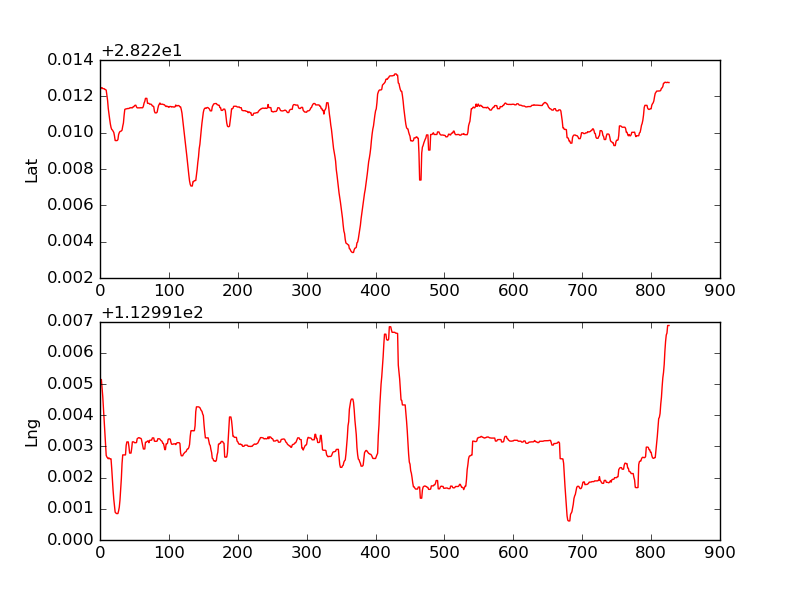
\includegraphics[height=4cm]{figure_4_mid_location1}}\hspace{4em}%
  \subfloat[均值滤波后的轨迹数据]{%
    \label{fig:3_2_2_1}
    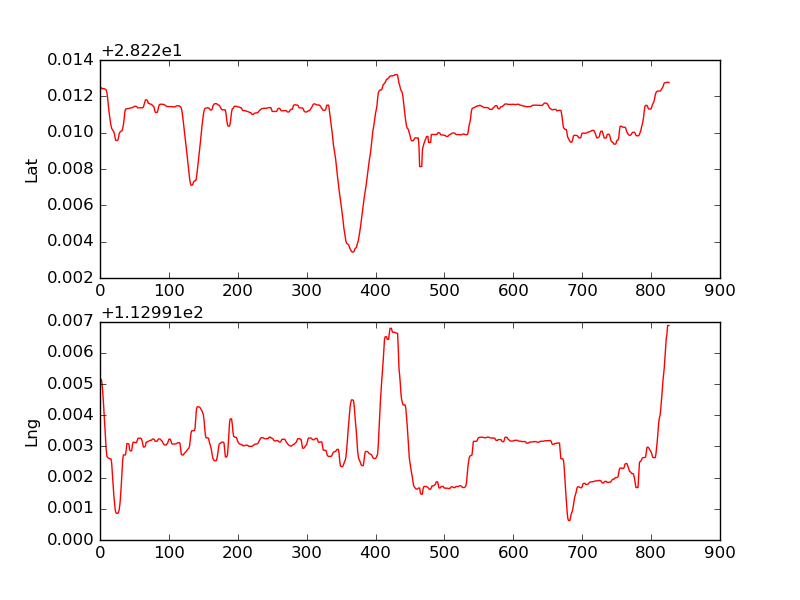
\includegraphics[height=4cm]{figure_4_mid_location1_avg}}
  \caption{轨迹均值滤波实验结果1}
  \label{fig:3_3_1}
\end{figure}
\begin{figure}[htb]
  \centering%
  \subfloat[原始轨迹数据]{%
    \label{fig:3_2_2_1}
    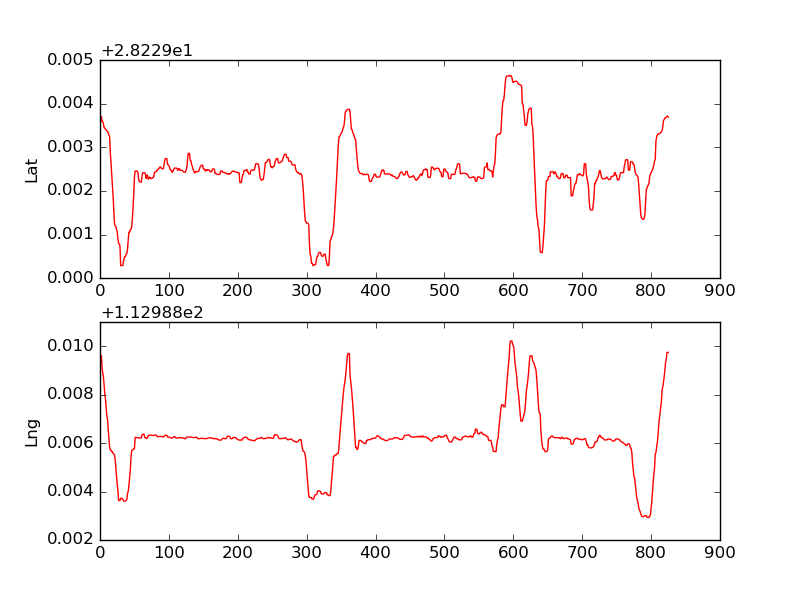
\includegraphics[height=4cm]{figure_4_mid_location2}}\hspace{4em}%
  \subfloat[均值滤波后的轨迹数据]{%
    \label{fig:3_2_2_2}
    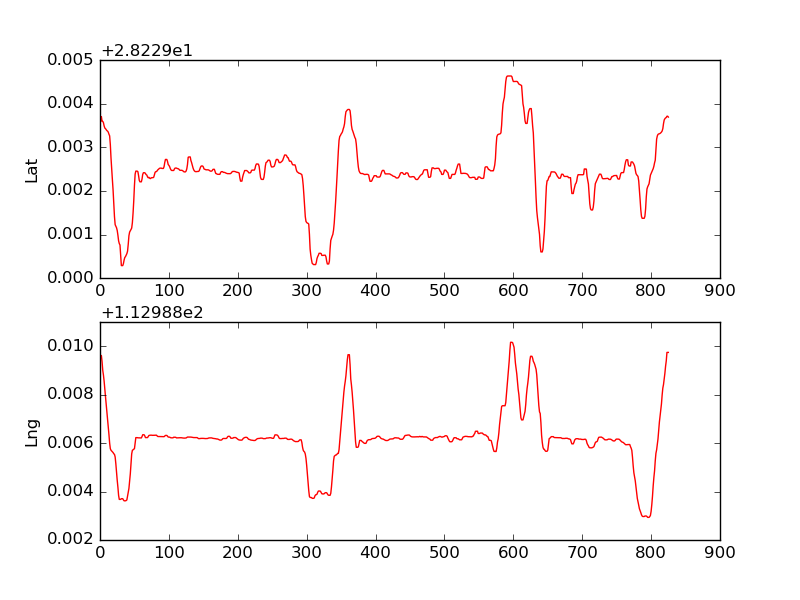
\includegraphics[height=4cm]{figure_4_mid_location2_avg}}
  \caption{轨迹均值滤波实验结果2}
  \label{fig:3_3_2}
\end{figure}
\par 通过对比观察滤波结果图可以发现,相对于中值滤波,均值滤波能够较好的平滑用户的轨迹变化曲线,剔除GPS漂移点。但是,同样无法很有效的处理漂移偏差大的位置点。
\par 通过采取卡尔曼滤波算法得到的用户轨迹如图\ref{fig:3_4_1}、\ref{fig:3_4_2},根据观察图中滤波后的用户轨迹数据,我们可以发现虽然图形变得平滑了许多,但是却使得原有的轨迹信息收到了模糊,难以有效的将两个用户轨迹进行相似度计算。
\begin{figure}[htb]
  \centering%
  \subfloat[原始轨迹数据]{%
    \label{fig:3_2_1_1}
    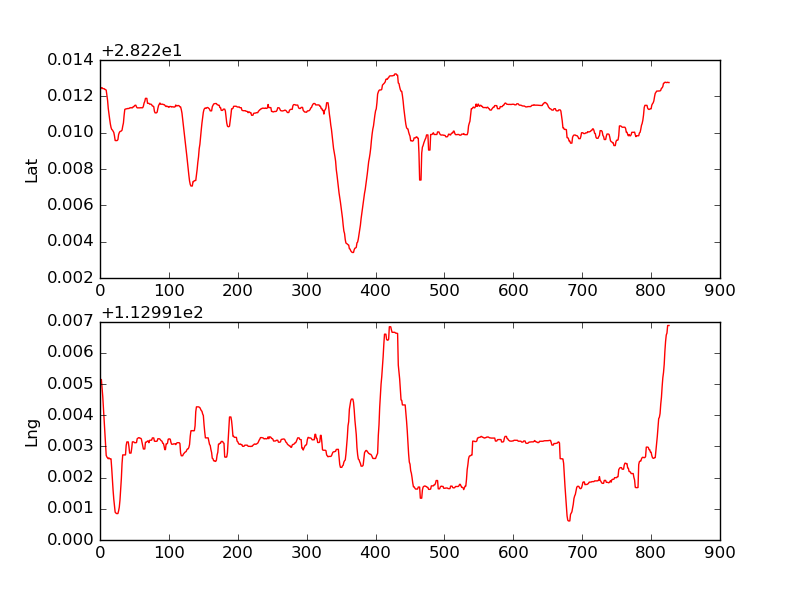
\includegraphics[height=4cm]{figure_4_mid_location1}}\hspace{4em}%
  \subfloat[卡尔曼滤波后的轨迹数据]{%
    \label{fig:3_2_2_1}
    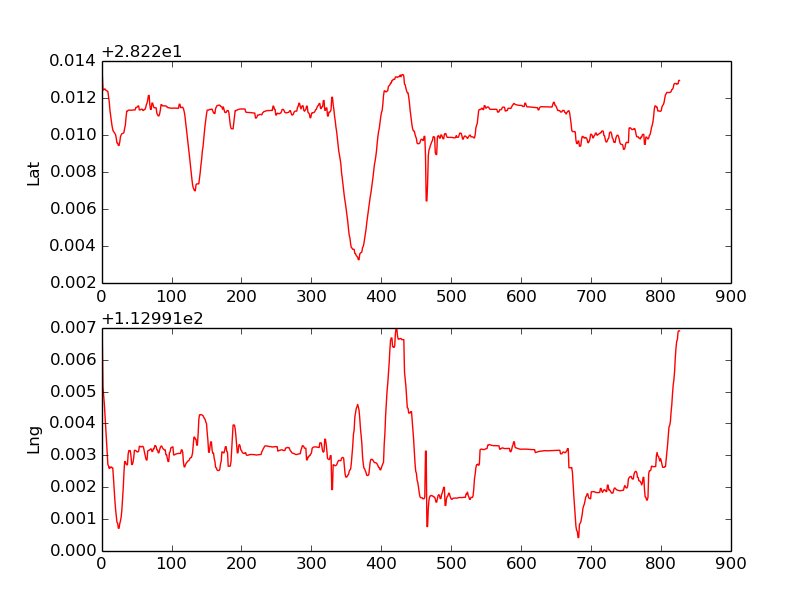
\includegraphics[height=4cm]{figure_4_mid_location1_kalman_ed}}
  \caption{卡尔曼滤波实验结果1}
  \label{fig:3_4_1}
\end{figure}
\begin{figure}[htb]
  \centering%
  \subfloat[原始轨迹数据]{%
    \label{fig:3_2_2_1}
    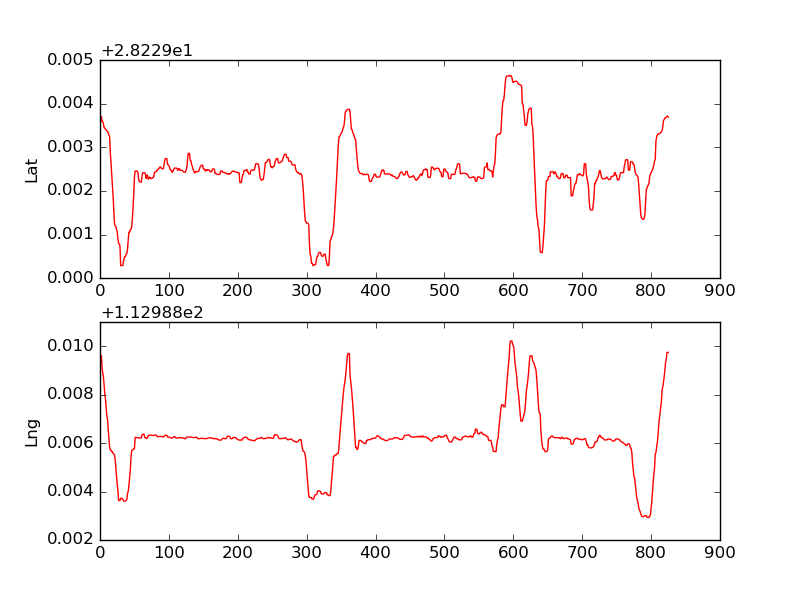
\includegraphics[height=4cm]{figure_4_mid_location2}}\hspace{4em}%
  \subfloat[卡尔曼滤波后的轨迹数据]{%
    \label{fig:3_2_2_2}
    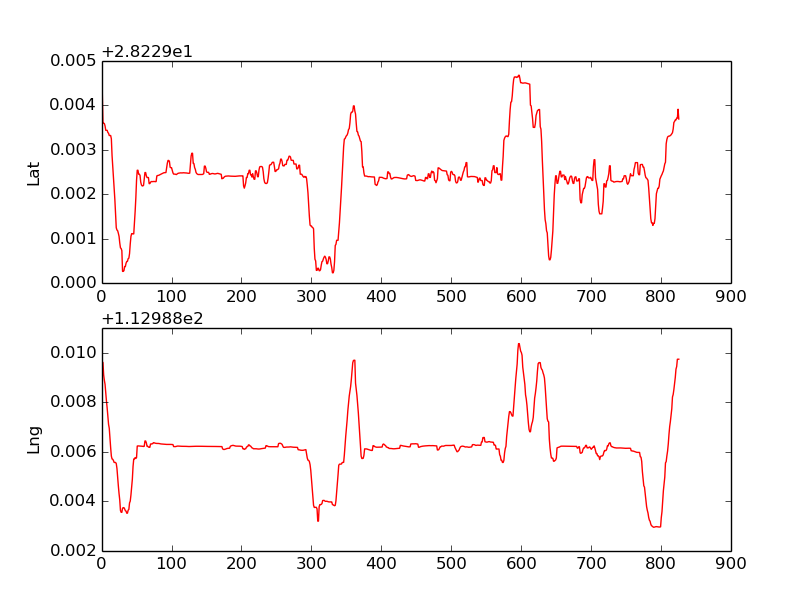
\includegraphics[height=4cm]{figure_4_mid_location2_kalman_ed}}
  \caption{卡尔曼滤波实验结果2}
  \label{fig:3_4_2}
\end{figure}
\par 在本研究中,我们采用了一种基于速度的分段卡尔曼滤波方法。考虑到在一个时间片内,如果当前位置点的速度和它之前的位置点的速度绝对差大于$\Delta v$ 时($\Delta v$作为一个未知的参数,需要我们在实际使用中给出)采用这样的方法将原有用户轨迹切分为$n$段然后针对每一段轨迹采用卡尔曼滤波算法,最终的部分轨迹滤波结果见图\ref{fig:3_5_1}、\ref{fig:3_5_2},可见经过按照速度分段后使用卡尔曼滤波能够比较好的过滤掉漂移点。
\begin{figure}[htb]
  \centering%
  \subfloat[原始轨迹数据]{%
    \label{fig:3_2_1_1}
    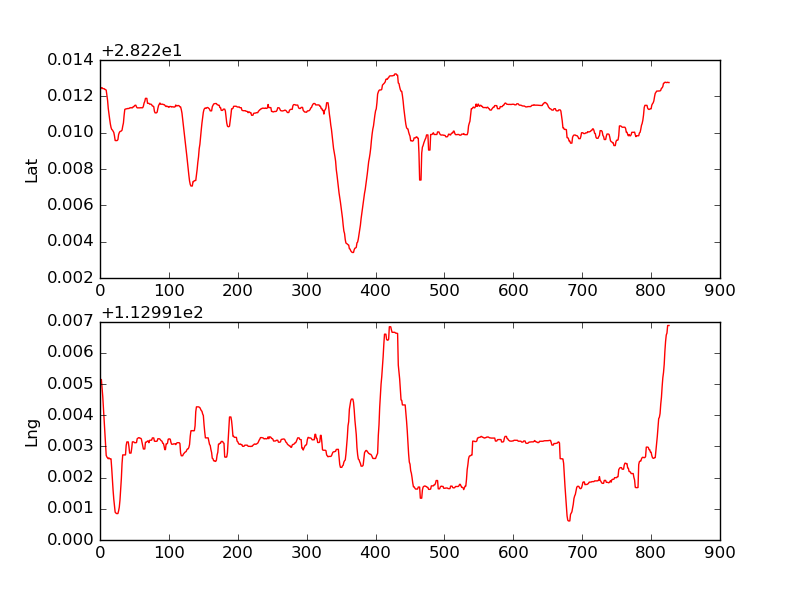
\includegraphics[height=4cm]{figure_4_mid_location1}}\hspace{4em}%
  \subfloat[分段卡尔曼滤波数据]{%
    \label{fig:3_2_2_1}
    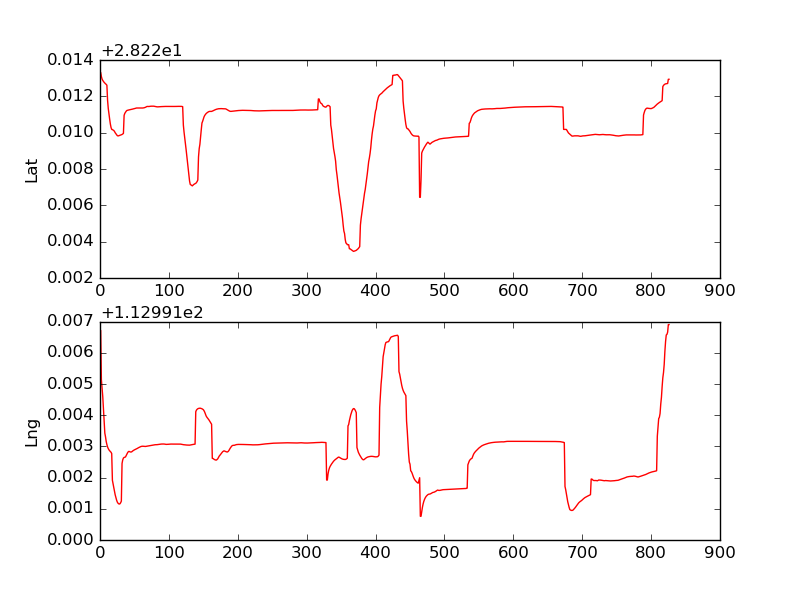
\includegraphics[height=4cm]{figure_4_mid_location1_kalman}}
  \caption{分段卡尔曼滤波轨迹结果1}
  \label{fig:3_5_1}
\end{figure}
\begin{figure}[htb]
  \centering%
  \subfloat[原始轨迹数据]{%
    \label{fig:3_2_2_1}
    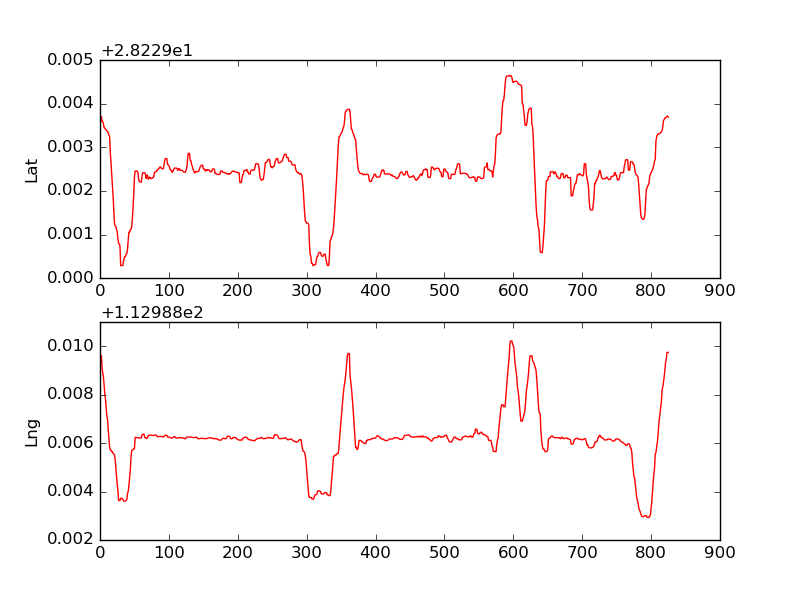
\includegraphics[height=4cm]{figure_4_mid_location2}}\hspace{4em}%
  \subfloat[分段卡尔曼滤波数据]{%
    \label{fig:3_2_2_2}
    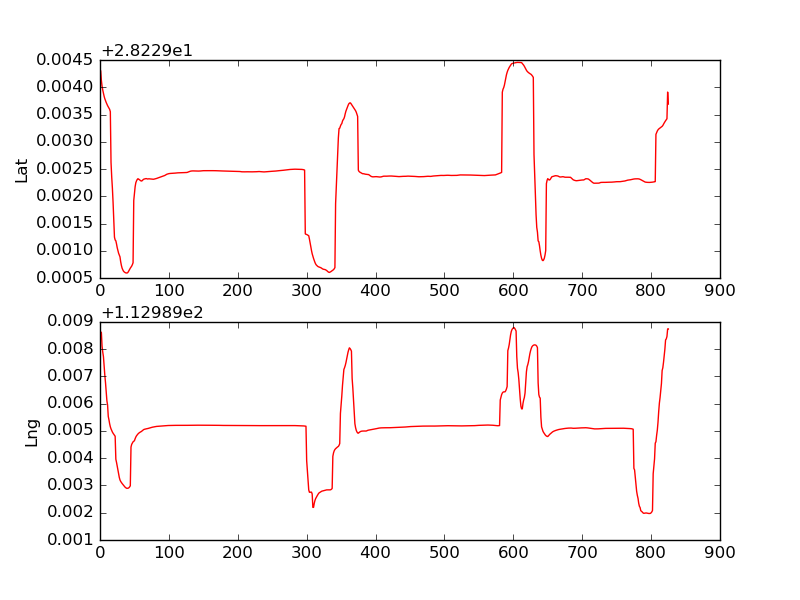
\includegraphics[height=4cm]{figure_4_mid_location2_kalman}}
  \caption{分段卡尔曼滤波轨迹结果2}
  \label{fig:3_5_2}
\end{figure}
\par 本小节主要针对前文中提及的三种常用的滤波算法进行了实验结果展示和效果分析,初步得出了使用卡尔曼滤波更加可行的判断结果。
\subsection{轨迹中停留点检测}
在实际生活中用户的轨迹是由一系列GPS点构成的,剔除其中的噪音点和用户在路上的点,能够从中挖掘出进一步信息的位置信息即为轨迹中的停留点,通常停留点并不是指用户轨迹中速度为零的点,而是由一组GPS 点构成区域,一个停留点通常对应现实生活中富有具体意义的点,能够更好的反映出用户之间轨迹的相似程度。如图\ref{fig:staypoint}所示,在现实生活中的停留点可以是一个具体的建筑名称,也可以是代表一个固定的区域,甚至可以是一个具有特殊意义的点。
\begin{figure}[htp]
\centering
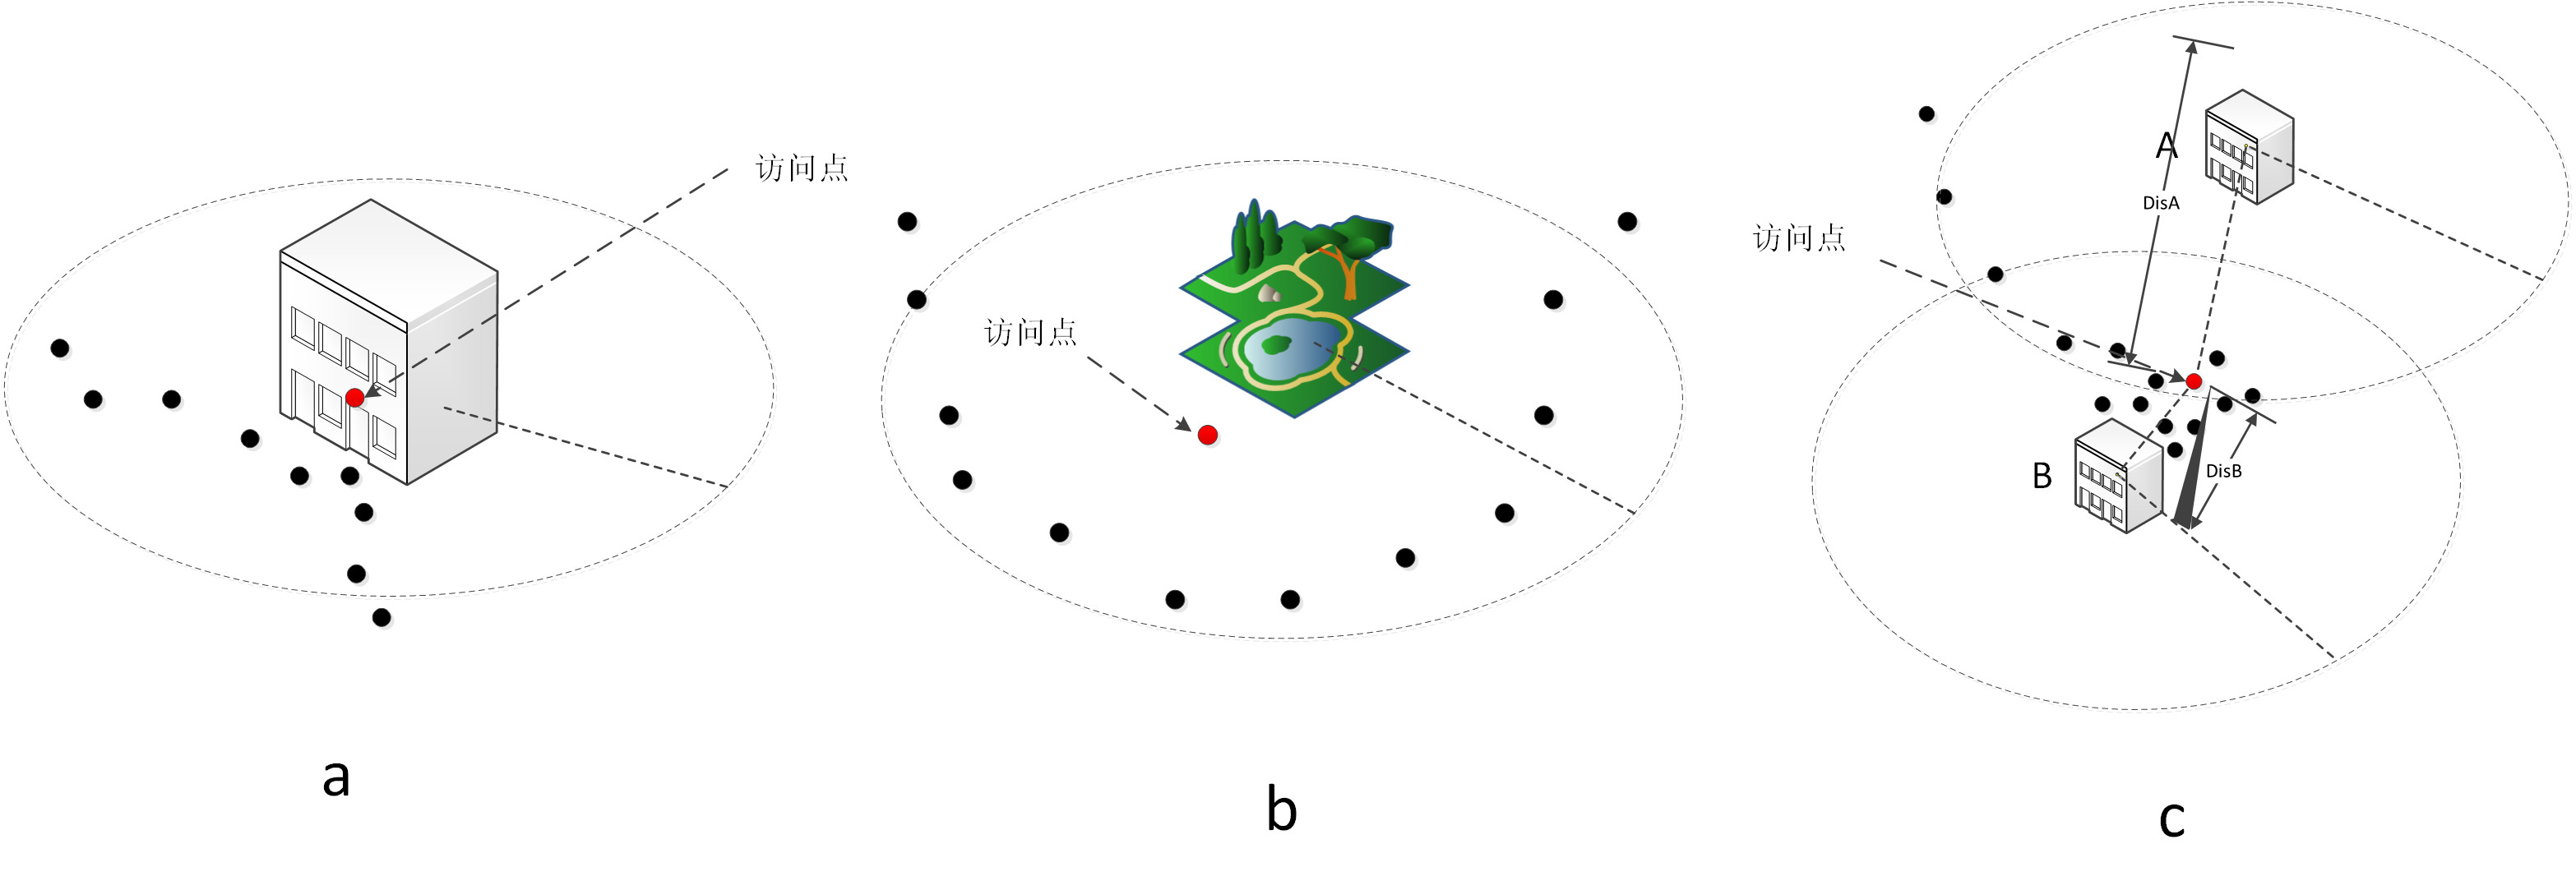
\includegraphics[width=0.8\textwidth]{figure_4_stay-points}
\caption{现实生活中的停留点示意图}
\label{fig:staypoint}
\end{figure}
\par 通过对停留点的识别,能够让我们更加深入的了解和认识用户的日常轨迹,同时从一个更加细粒度的层次来分析用户之间的轨迹相似度,停留点检测实验结果如图\ref{fig:SP_1}、\ref{fig:SP_2}所示,图中所得到的每一个停留点都具有丰富的现实意义,能够有效地表示用户访问的地点、位置。
\begin{figure}[htb]
  \centering%
  \subfloat[原始轨迹数据]{%
    \label{fig:3_3_1_1}
    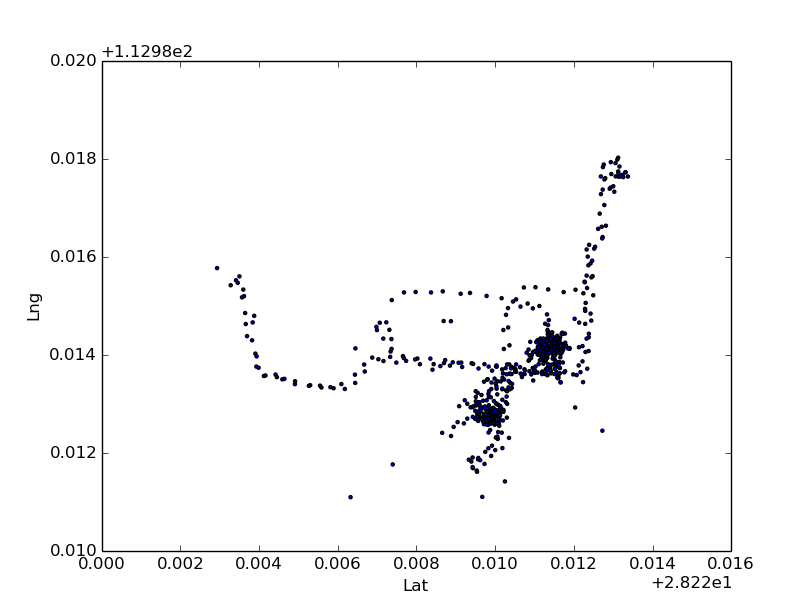
\includegraphics[height=4cm]{figure_4_location1_scater}}\hspace{4em}%
  \subfloat[检测出的停留点]{%
    \label{fig:sp_1}
    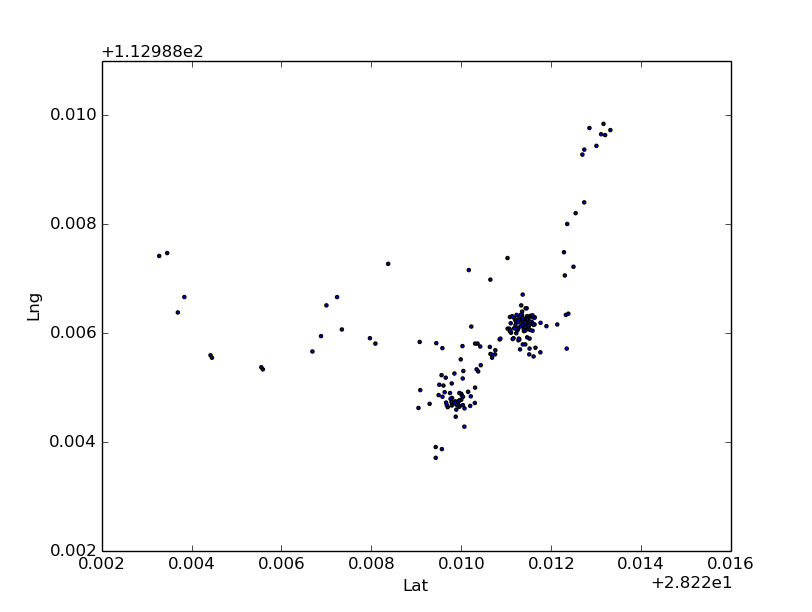
\includegraphics[height=4cm]{figure_4_location1_sp}}
  \caption{停留点检测实验结果1}
  \label{fig:SP_1}
\end{figure}
\begin{figure}[htb]
  \centering%
  \subfloat[原始轨迹数据]{%
    \label{fig:3_3_1_1}
    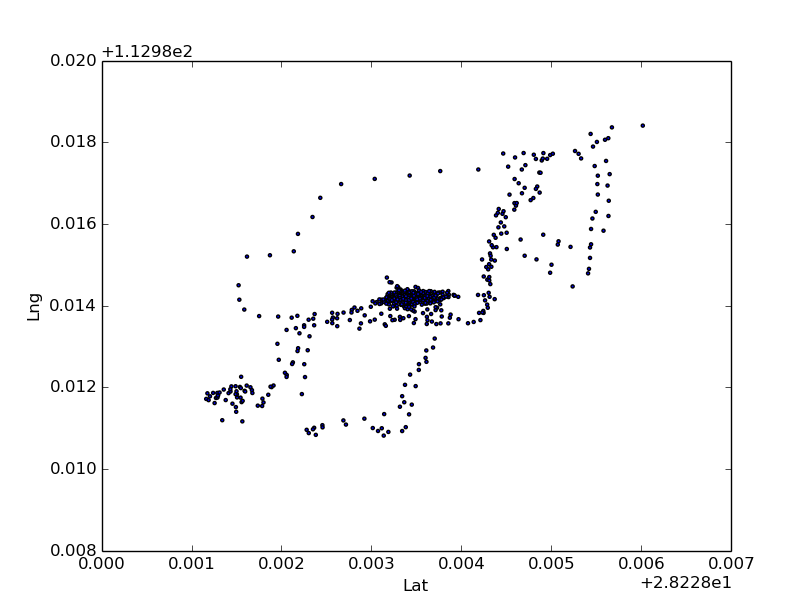
\includegraphics[height=4cm]{figure_4_location2_scater}}\hspace{4em}%
  \subfloat[检测出的停留点]{%
    \label{fig:sp_2}
    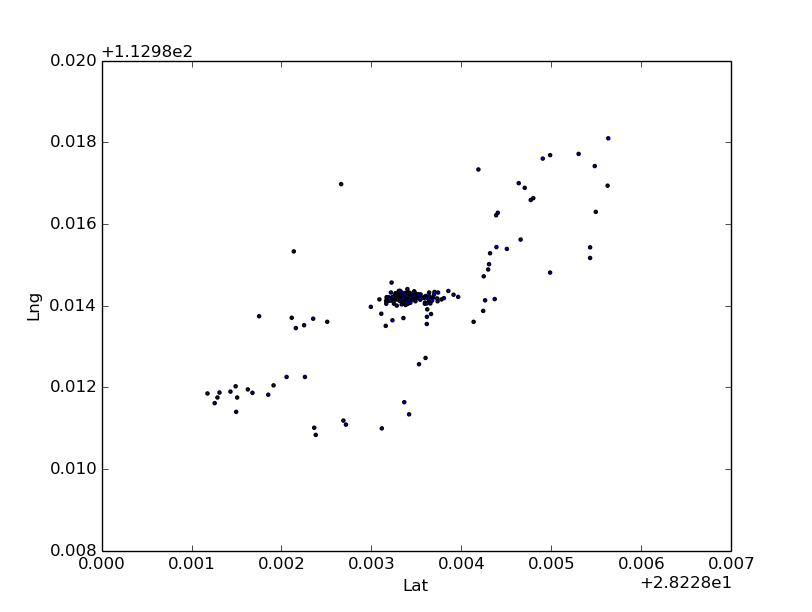
\includegraphics[height=4cm]{figure_4_location2_sp}}
  \caption{停留点检测实验结果2}
  \label{fig:SP_2}
\end{figure}
\subsection{用户轨迹停留点聚类}
\label{traclustar}
本节针对上面得到的用户轨迹中的停留点,采用不同的聚类算法所得到的不同的聚类结果进行描述。在前面的章节中我们详细介绍了聚类中常用的三种算法K-means聚类、DJ-Cluster的密度聚类和最新发表的改进的密度聚类算法,接下来我们将在实验中对这三种聚类算法进行比较。
\par 首先我们对用户轨迹数据采用K-means算法进行聚类实验,但是K-means聚类算法具有以下的明显的缺点:首先是K-means聚类结果依赖于参数$k$的初始化,其中$k$是指聚类个数。$k$个数的确定往往是靠经验值设定;其次是K-means算法初始化时聚类中心的选择,因为该算法采用的随机初始化聚类中心点,中心点选择不同会导致聚类的结果也出现差异甚至影响聚类的时间复杂度,使得聚类结果容易得到局部最优解而非全局最优解;最后的一个缺点是K-means聚类算法对原始数据中的噪音点和离群点非常敏感,聚类结果很容易受到离群点的影响从而导致簇的偏移。
\par 在本研究中因为是针对用户的空间轨迹进行聚类分析,而现实生活中用户的停留点主要是以相隔距离比较大的建筑等,因此在采用K-means聚类过程中,对噪音点的影响基本可以忽略不计,最主要的就是考虑不同的参数$k$对最终聚类结果的影响,图\ref{fig:3_8_1}、\ref{fig:3_8_2}主要展示不同的参数$k$取值对最终轨迹聚类结果的影响。图\ref{fig:3_9_1}、\ref{fig:3_9_2}在地图上标记了在不同参数$k$取值情况下的簇中心使得能够有更加直观的观察。
\begin{figure}[htb]
  \centering%
  \subfloat[原始轨迹数据]{%
    \label{fig:3_8_1_1}
    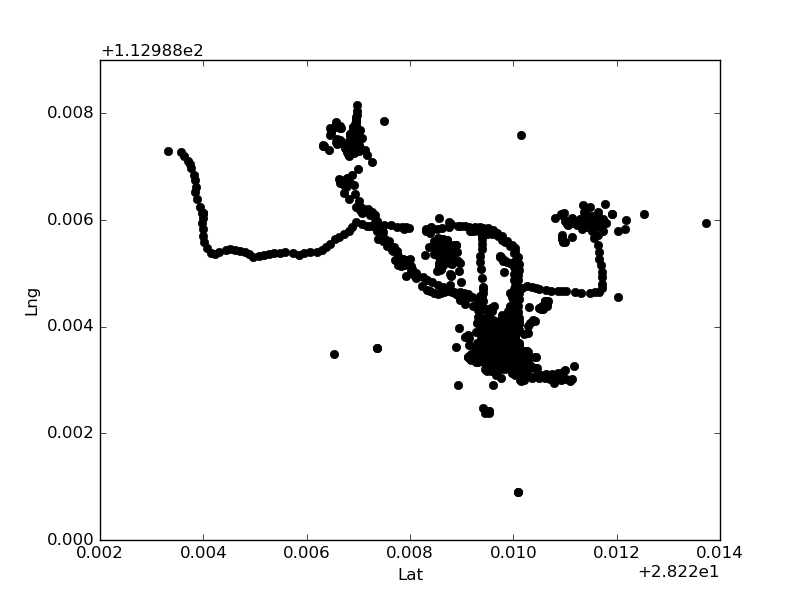
\includegraphics[height=5cm]{figure4_tra1}}%\hspace{4em}
  \subfloat[参数k=3]{%
    \label{fig:3_8_1_2}
    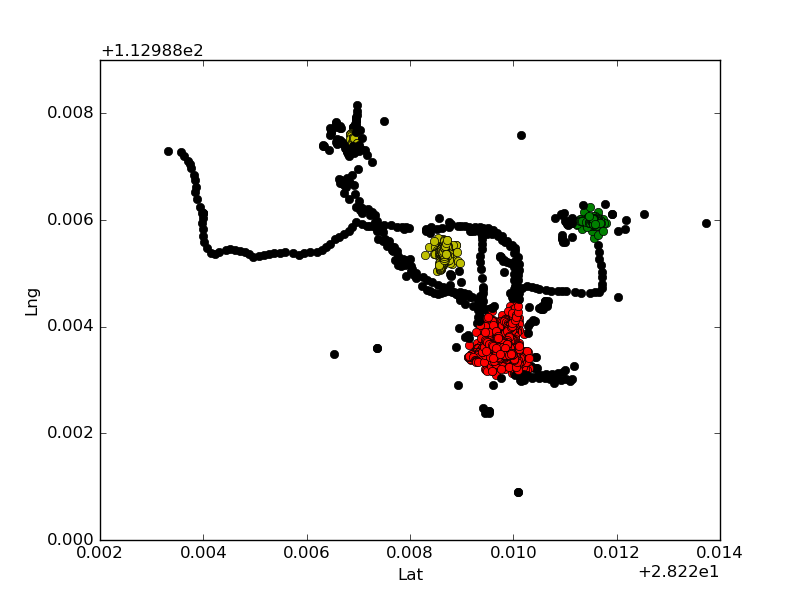
\includegraphics[height=5cm]{figure4_tra1_kmeans_3}}\\
  \subfloat[参数k=4]{%
    \label{fig:3_8_1_3}
    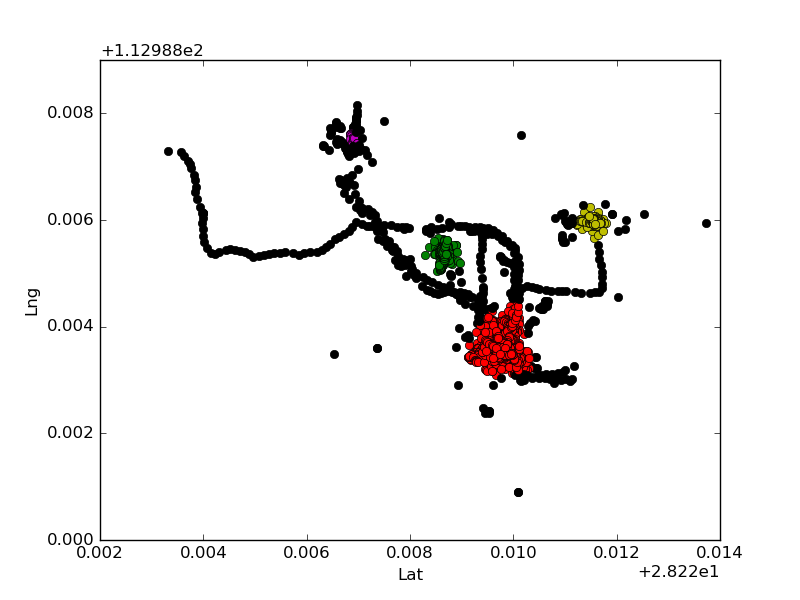
\includegraphics[height=5cm]{figure4_tra1_kmeans_4}}
  \subfloat[参数k=5]{%
    \label{fig:3_8_1_4}
    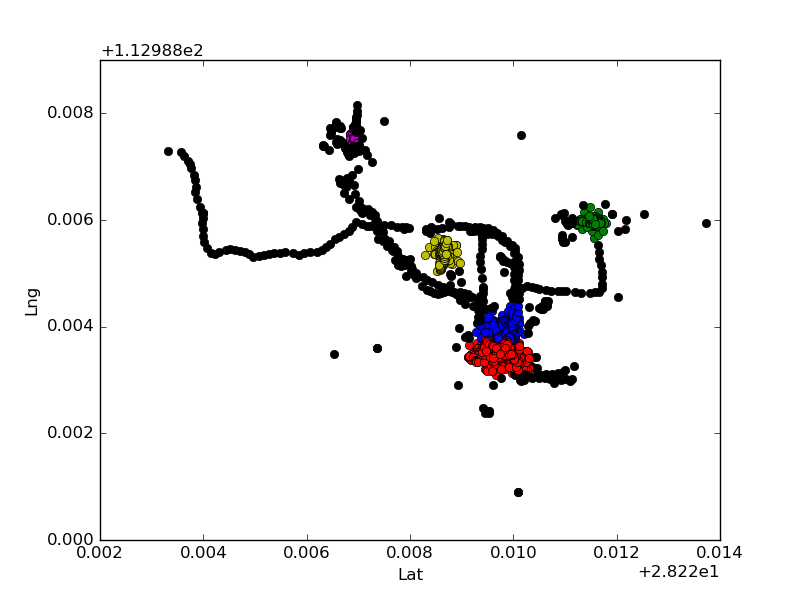
\includegraphics[height=5cm]{figure4_tra1_kmeans_5}}
  \caption{基于K-means的轨迹聚类实验结果1}
  \label{fig:3_8_1}
\end{figure}
\begin{figure}[htb]
  \centering%
  \subfloat[原始轨迹数据]{%
    \label{fig:3_9_1_1}
    \includegraphics[height=6cm]{figure4_tra1_map}}%\hspace{4em}
  \subfloat[参数k=3]{%
    \label{fig:3_9_1_2}
    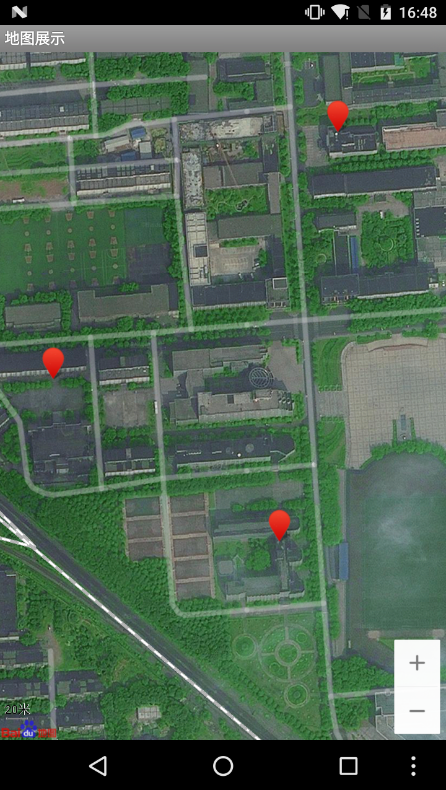
\includegraphics[height=6cm]{figure4_tra1_map_k3}}
  \subfloat[参数k=4]{%
    \label{fig:3_9_1_3}
    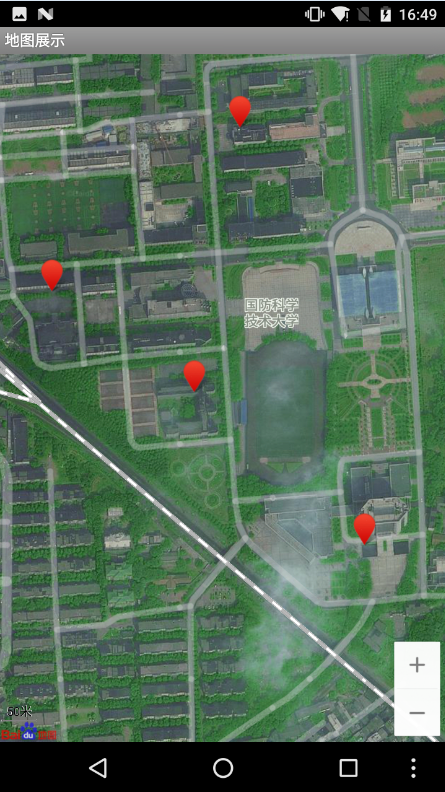
\includegraphics[height=6cm]{figure4_tra1_map_k4}}
  \subfloat[参数k=5]{%
    \label{fig:3_9_1_4}
    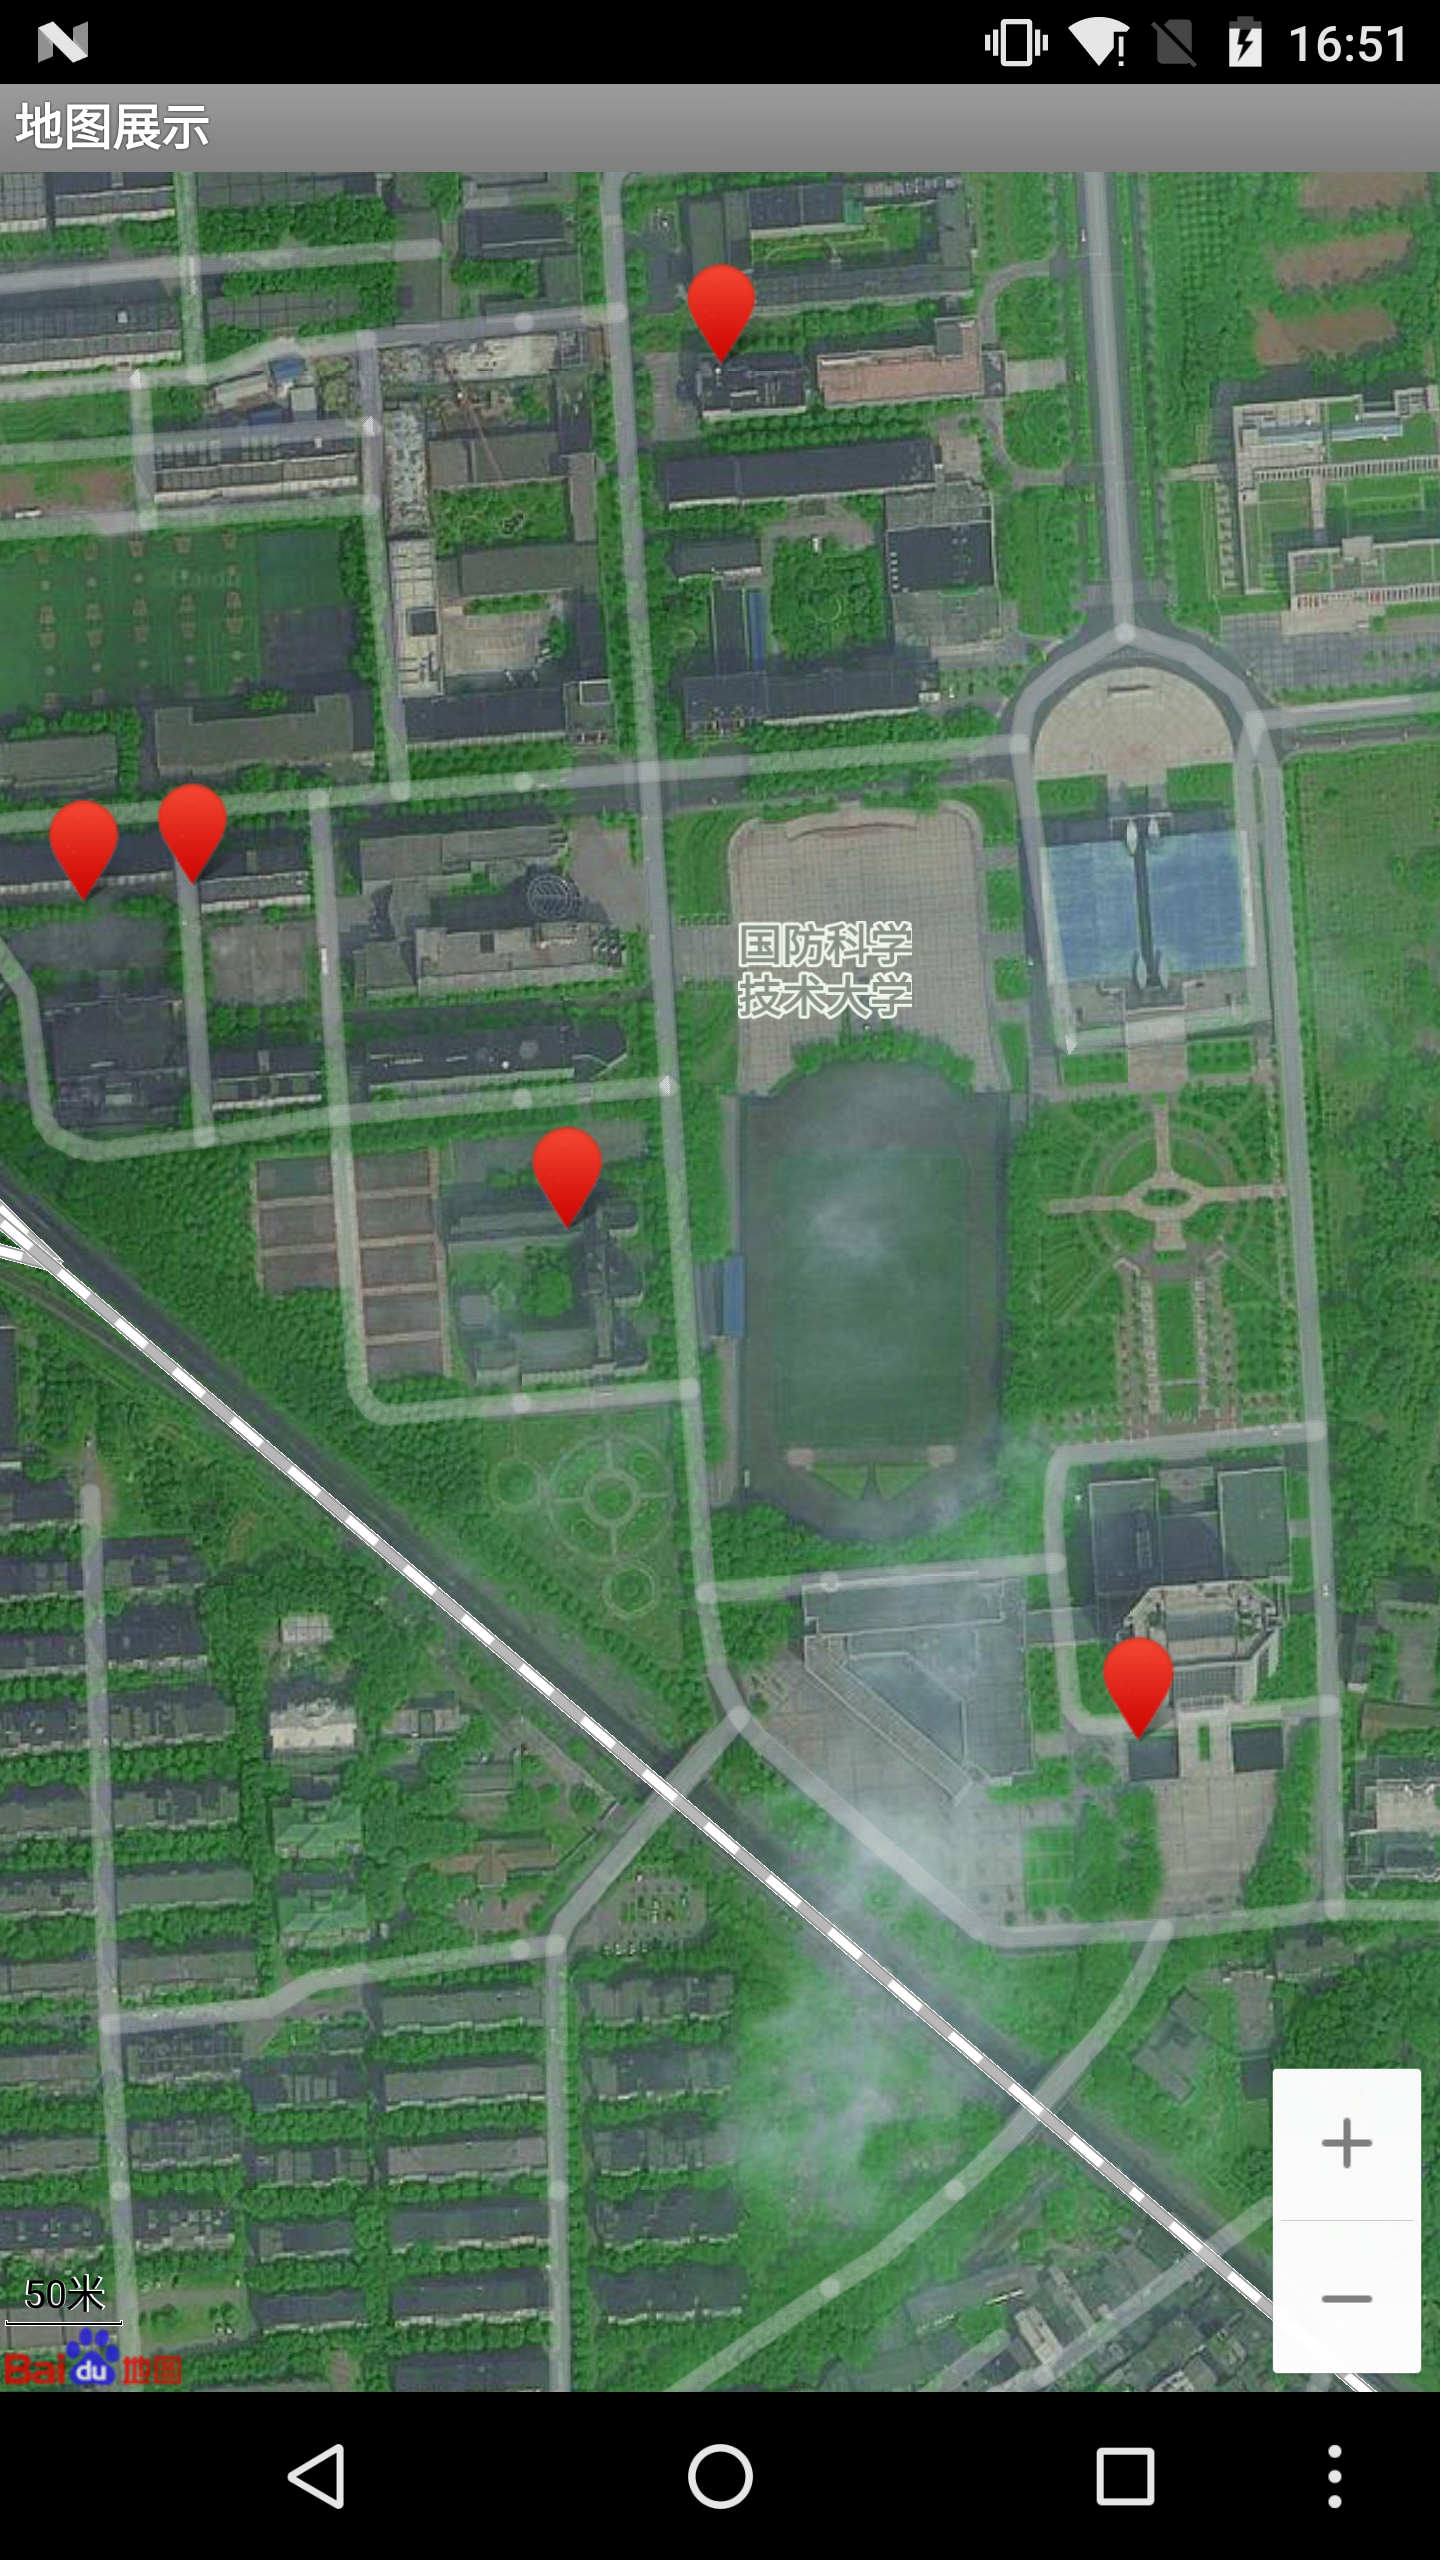
\includegraphics[height=6cm]{figure4_tra1_map_k5}}
  \caption{基于K-means的轨迹聚类实验结果地图展示1}
  \label{fig:3_9_1}
\end{figure}
\begin{figure}[htb]
  \centering%
  \subfloat[原始轨迹数据]{%
    \label{fig:3_8_2_1}
    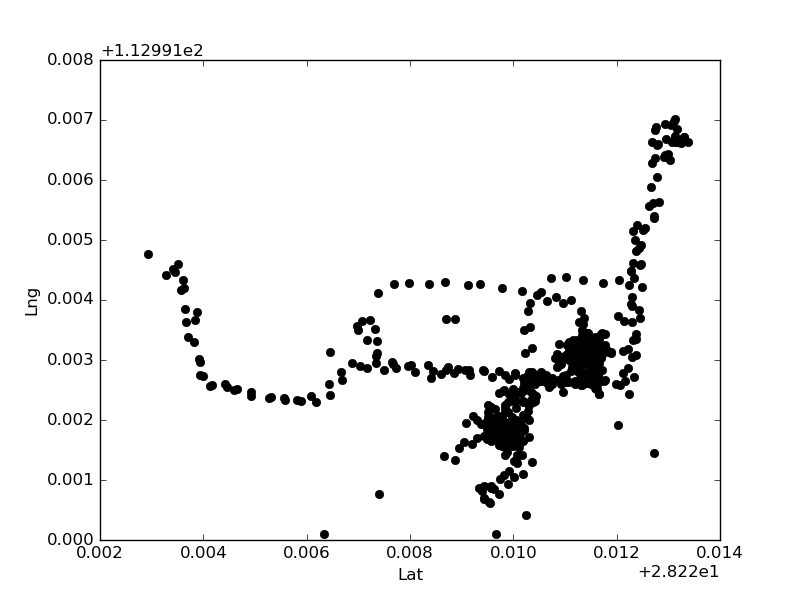
\includegraphics[height=5cm]{figure4_tra2}}%\hspace{4em}
  \subfloat[参数k=3]{%
    \label{fig:3_8_2_2}
    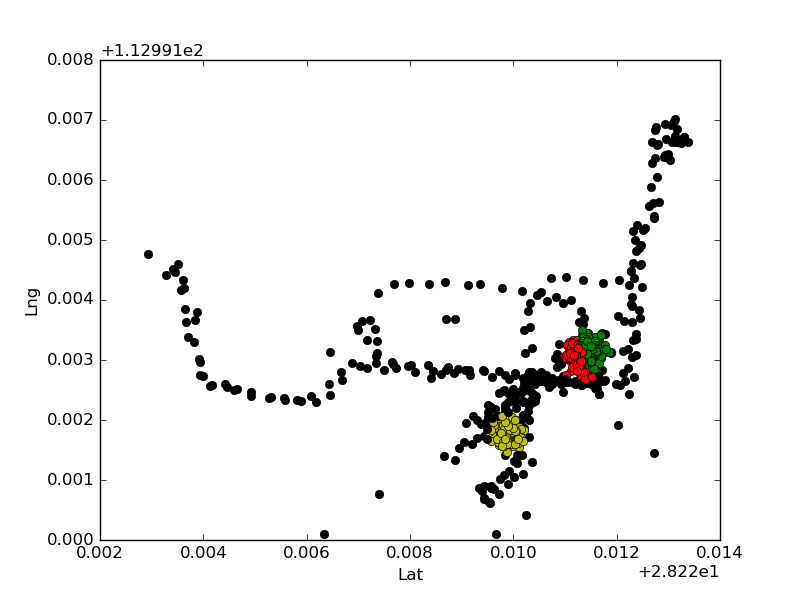
\includegraphics[height=5cm]{figure4_tra2_kmeans_3}}\\
  \subfloat[参数k=4]{%
    \label{fig:3_8_2_3}
    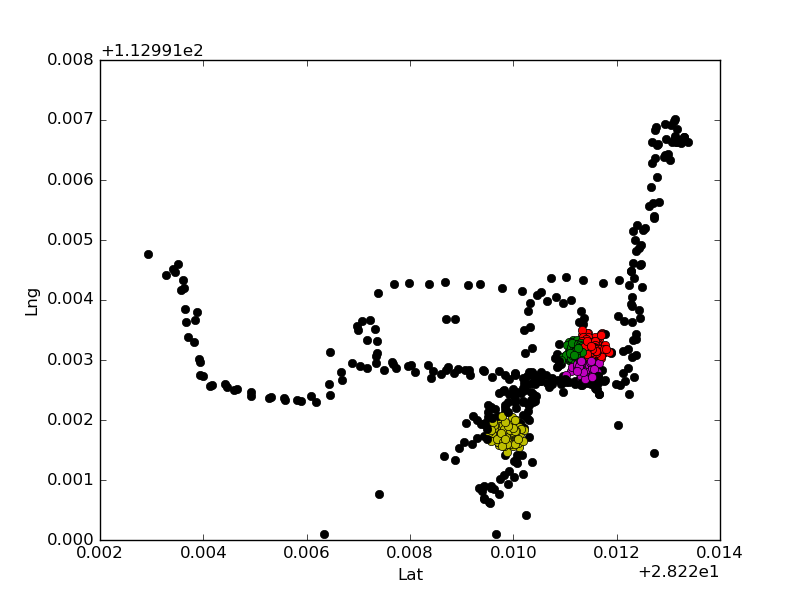
\includegraphics[height=5cm]{figure4_tra2_kmeans_4}}
  \subfloat[参数k=5]{%
    \label{fig:3_8_2_4}
    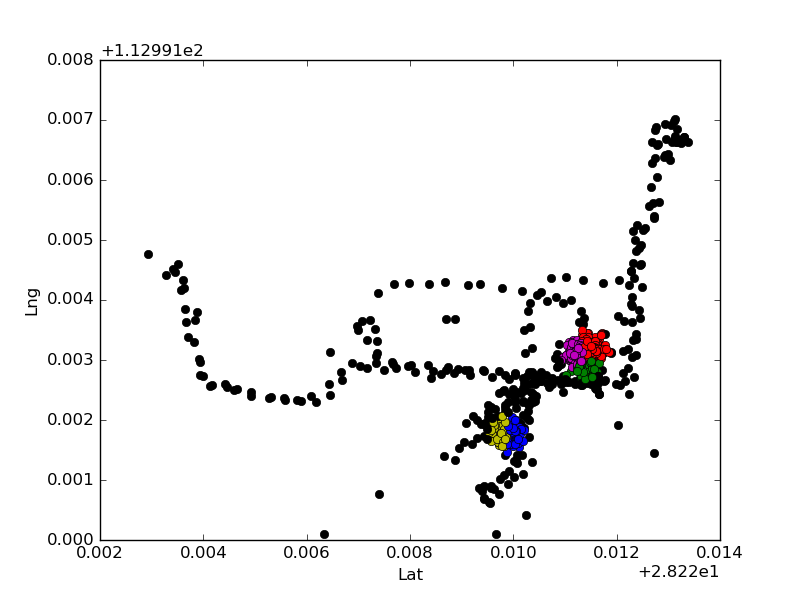
\includegraphics[height=5cm]{figure4_tra2_kmeans_5}}
  \caption{基于K-means的轨迹聚类实验结果2}
  \label{fig:3_8_2}
\end{figure}
\begin{figure}[htb]
  \centering%
  \subfloat[原始轨迹数据]{%
    \label{fig:3_9_2_1}
    \includegraphics[height=6cm]{figure4_tra2_map}}%\hspace{4em}
  \subfloat[参数k=3]{%
    \label{fig:3_9_2_2}
    \includegraphics[height=6cm]{figure4_tra2_map_k3}}
  \subfloat[参数k=4]{%
    \label{fig:3_9_2_3}
    \includegraphics[height=6cm]{figure4_tra2_map_k4}}
  \subfloat[参数k=5]{%
    \label{fig:3_9_2_4}
    \includegraphics[height=6cm]{figure4_tra2_map_k5}}
  \caption{基于K-means的轨迹聚类实验结果地图展示2}
  \label{fig:3_9_2}
\end{figure}
\par 通过对轨迹数据的聚类分析我们可以得知,如果在聚类前我们能够确切的知道用户的轨迹数据应该划分的簇的个数,那么K-means聚类算法将会得出非常合理的结果,我们在观察图\ref{fig:3_9_1}、\ref{fig:3_9_2}时发现,当簇的个数越接近符合用户访问位置个数的时候,那么聚类点将更能够反映出真实的情况,在图\ref{fig:3_11_1}中,(a)所对应的聚类得到的簇包含了实际上没有正确的将用户访问过的位置区分开,因为这两个访问的位置距离相隔太近,导致K-means算法将这两个簇合并为一个簇,但是如果我们将聚类个数设置为5就能够成功的识别出这两个位置。在另一实验结果图\ref{fig:3_11_2}中也出现了类似的情况。但是根据图中实验情况分析发现对于一部分在路上的点被划分到了聚类簇中,同时有些应该被单独聚类成一个独立的簇的点被划分到了在路上的点中,这些都是因为我们无法正确的给出符合当前轨迹访问点个数的聚类个数所造成的。
\par 接下来将会基于DJ-Cluster 算法来对轨迹数据进行聚类并对结果进行分析。DJ-Cluster算法是基于密度聚类算法DBSCAN而改进的一种密度聚类算法,通过利用密度相连的原理可以发现任意形状的簇,但是算法存在有一个局限性:算法的性能和准确性依赖于参数$Eps$(邻域半径)和$MinPts$(最少点数量),如果邻域半径的取值过大那么所有的点将会划分为同一个簇,因此在实际的使用过程中,需要不断地对参数进行调整才能得到比较理想的结果,如图\ref{fig:3_10_1}、\ref{fig:3_10_2}结果所示,实际地图中结果展示如图\ref{fig:3_11_1}、\ref{fig:3_11_2}所示。
\begin{figure}[htb]
  \centering%
  \subfloat[原始轨迹数据]{%
    \label{fig:3_10_1_1}
    \includegraphics[height=4cm]{figure4_tra_for_dj_1}}\hspace{4em}%
  \subfloat[DJ-Cluster聚类结果]{%
    \label{fig:3_10_1_2}
    \includegraphics[height=4cm]{figure4_tra_result_dj_1}}
  \caption{基于DJ-Cluster的轨迹聚类实验结果1}
  \label{fig:3_10_1}
\end{figure}
\begin{figure}[htb]
  \centering%
  \subfloat[原始轨迹数据]{%
    \label{fig:3_11_1_1}
    \includegraphics[height=6cm]{figure4_tra_map_dj1}}\hspace{4em}%
  \subfloat[DJ-Cluster聚类结果]{%
    \label{fig:3_11_1_2}
    \includegraphics[height=6cm]{figure4_tra_map_result_dj_1}}
  \caption{基于DJ-Cluster的轨迹聚类实验结果地图展示1}
  \label{fig:3_11_1}
\end{figure}
\begin{figure}[htb]
  \centering%
  \subfloat[原始轨迹数据]{%
    \label{fig:3_10_2_1}
    \includegraphics[height=4cm]{figure4_tra_for_dj_2}}\hspace{4em}%
  \subfloat[DJ-Cluster聚类结果]{%
    \label{fig:3_10_2_2}
    \includegraphics[height=4cm]{figure4_tra_result_dj_2}}
  \caption{基于DJ-Cluster的轨迹聚类实验结果2}
  \label{fig:3_10_2}
\end{figure}
\begin{figure}[htb]
  \centering%
  \subfloat[原始轨迹数据]{%
    \label{fig:3_11_2_1}
    \includegraphics[height=6cm]{figure4_tra_map_dj2}}\hspace{4em}%
  \subfloat[DJ-Cluster聚类结果]{%
    \label{fig:3_11_2_2}
    \includegraphics[height=6cm]{figure4_tra_map_result_dj_2}}
  \caption{基于DJ-Cluster的轨迹聚类实验结果地图展示2}
  \label{fig:3_11_2}
\end{figure}
\par 通过观察结果地图展示和原始数据对比能够发现,相比于K-means算法DJ-Cluster能够得到比较正确的结果,但是结果依赖于对前面所描述的参数的不断调整。从图\ref{fig:3_11_1}中(a)中描绘的用户位置点集合(b)中得到的聚类结果进行分析,右上角是宿舍区域,因为当前点比较少,未能够正确的将这个区域聚类成一个单独的簇进行标记。但是从图\ref{fig:3_11_2}中发现DJ-Cluster基本得到了非常好的聚类结果。受限于DJ-Cluster算法对参数的敏感性,接下来将介绍一种新的聚类算法,该算法将大大降低对参数和数据的依赖性。
\par 接下来进一步展示在Science上发表的聚类算法,该算法通过结合现实理论,假设聚类的中心实质上是有局部密度低的点所环绕的,并且这点和另外密度高的点距离都比较大。这样通过计算得到每个点的当前密度值后根据划分的边界阈值进行密度点的划分,找出每个块中密度最大的点并将其周围密度小于该点密度的点加入到当前簇中得到最终的聚类结果。该算法因为考虑当将点密度排序后进行处理,保持了点密度顺序的相对稳定的同时减小了半径阈值带来的影响。聚类算法的具体的实验结果见图\ref{fig:3_12_1}、\ref{fig:3_12_2},将聚类结果通过地图展示如图\ref{fig:3_13_1}、\ref{fig:3_13_2}所示,从图\ref{fig:3_12_1}中可以观察到聚类结果是比较
\begin{figure}[htb]
  \centering%
  \subfloat[原始轨迹数据]{%
    \label{fig:3_12_1_1}
    \includegraphics[height=4cm]{figure4_tra_for_science1}}\hspace{4em}%
  \subfloat[聚类结果]{%
    \label{fig:3_12_1_2}
    \includegraphics[height=4cm]{figure4_science_1_cluster}}
  \caption{轨迹聚类实验结果展示1}
  \label{fig:3_12_1}
\end{figure}
\begin{figure}[htb]
  \centering%
  \subfloat[原始轨迹数据]{%
    \label{fig:3_13_1_1}
    \includegraphics[height=6cm]{figure4_tra_map_science1}}\hspace{4em}%
  \subfloat[聚类结果]{%
    \label{fig:3_13_1_2}
    \includegraphics[height=6cm]{figure4_tra_map_result_science1}}
  \caption{轨迹聚类实验结果地图表示1}
  \label{fig:3_13_1}
\end{figure}
\begin{figure}[htb]
  \centering%
  \subfloat[原始轨迹数据]{%
    \label{fig:3_12_2_1}
    \includegraphics[height=4cm]{figure4_tra_for_science2}}\hspace{4em}%
  \subfloat[聚类结果]{%
    \label{fig:3_12_2_2}
    \includegraphics[height=4cm]{figure4_science_2_cluster}}
  \caption{轨迹聚类实验结果展示2}
  \label{fig:3_12_2}
\end{figure}
\begin{figure}[htb]
  \centering%
  \subfloat[原始轨迹数据]{%
    \label{fig:3_13_2_1}
    \includegraphics[height=6cm]{figure4_tra_map_science2}}\hspace{4em}%
  \subfloat[聚类结果]{%
    \label{fig:3_13_2_2}
    \includegraphics[height=6cm]{figure4_tra_map_result_science2}}
  \caption{轨迹聚类实验结果地图表示2}
  \label{fig:3_13_2}
\end{figure}
\par 通过分析图\ref{fig:3_12_1}和图\ref{fig:3_12_1}中的聚类结果发现该聚类算法能够比较正确的将用户的轨迹数据进行聚类同时也不依赖于太敏感的参数输入。在图\ref{fig:3_12_1}中用户正确访问的地方应该是五个,虽然(b)中的聚类结果也得出了五个簇中心位置,但是未能将寝室这一簇识别出来而是将在体育馆周围的点标注为聚类簇。虽然在最终的结果上有的会出现一点误差,但是能够去除对数据和参数的敏感性减少对实验的干预,在本研究中显得更加难能可贵和适用。
%\par 通过以上的实验方法,我们在得到用户的停留点和聚类轨迹之后,将会采用语义标签数据库和反地理编码查询相结合的手段进行轨迹语义化处理,假设得到了用户一天的轨迹数据并且进行了停留点切分和聚类得到了100个位置,而我们的语义标签数据库中只能够查询到其中的70个位置的语义标签,因此剩下的30个位置我们将采用反地理编码进行语义化,并将相对于的语义标签存入到语义数据库中避免二次调用反地理编码接口。
\par 本小节主要讨论了前面一章节中介绍的聚类算法在本研究中对用户轨迹聚类的效果以及每种聚类算法对参数的依赖以及影响,然后分析每一种聚类算法各自的优缺点,K-means聚类结果虽然比较好但是需要预先设定聚类个数,最明显的问题是我们收集的用户轨迹数据中无法预先知晓用户轨迹所应该聚类的个数,导致结果出现偏差;DJ-Cluster聚类算法同样存在类似的问题。本课题采用针对小数据进行聚类,一方面是因为数据量小比较容易发现较小的聚类簇,能够识别用户更加细粒度的访问位置,如果将用户多天的轨迹数据进行聚类,有可能将会导致较大数量的簇无法识别。另外采用小数据量时间切片进行分析聚类能够保证当前用户的某个聚类没有识别而下一段数据分析识别出来,形成效果叠加也能够保证最终结果的相对稳定,下一节将简要讨论如何对用户的轨迹点进行语义化。
\subsection{对用户轨迹的语义位置添加语义标签}
\label{sec:section3-3}
\par 在上面的小节中主要讲述了针对用户原始GPS轨迹数据进行滤波处理、轨迹停留点挖掘以及针对用户轨迹进行聚类。但是仅仅得到用户的空间轨迹信息是不够的,为此我们需要将用户轨迹中有意义的点添加上语义标签如图\ref{fig:tra_senantic}所示,为用户轨迹中的停留点加上语义标签,得能有助于我们了解用户去了什么地方,这些地方属于什么类型等。语义轨迹有助于我们进一步分析用户之间的相似性,因此本小节将介绍如何添加语义轨迹。
\par 现有的大多数工作是基于反地理编码技术来将空间轨迹语义化,将用户的位置转换为具体的道路门牌号等(如德雅路138号),然而有时候道路地址无法有效地表示用户位置的现实意义;另外的方法采用了机器学习的方法,首选从用户的轨迹中提取用户的位置点以及位置点的类型,采用关系马尔科夫网模型,利用网中的节点表示用户的访问点,基于条件随机场对用户的访问点进行推测得到用户的访问点的语义标签,但是采用机器学习效率较低,同时最终结果还受限于数据训练集,不适合普适计算的要求。因此我们采用了以语义标签数据库为主,反地理编码为辅的语义化方法。语义标签数据库中覆盖了本研究对象校园内部及其周边大部分语义位置点,假设得到了用户一天的轨迹数据并且进行了停留点切分和聚类得到了100个位置,而我们的语义标签数据库中只能够查询到其中的70个位置的语义标签,因此剩下的30个位置我们将采用反地理编码进行语义化,并将相对于的语义标签存入到语义数据库中避免二次调用反地理编码接口。如图\ref{fig:tra_senantic}所示,我们采用了三层了轨迹语义化处理模型,在最底层为用户的原始轨迹数据,中间层为上一小节中我们识别出的用户停留点或者聚类簇,最上层为用户的访问地点语义标签。
\begin{figure}[htp]
\centering
\includegraphics[width=0.8\textwidth]{figure_4_stay-point_semantic}
\caption{位置语义标签示意图}
\label{fig:tra_senantic}
\end{figure}
\par 在语义化的过程中,我们首先构建了一个符合当前范围内的语义标签数据库,里面包含了学校内部各个位置语义点以及学校周边大部分的位置语义信息,在为用户轨迹添加语义标签时,首先查找语义标签数据库内是否有相匹配的位置点。具体的匹配过程如图\ref{fig:matchlabel}所示,图中首先我们需要人为设定一个距离阈值,用来衡量当前位置点与语义标签位置点之间的关系。图\ref{fig:matchlabel}中a所示:当停留点或簇中心点距离语义标签库中有且仅有一个位置点的距离小于设定的阈值,则把当前语义标签赋予给当前位置;若如图\ref{fig:matchlabel}中b所示,当半径阈值内不止一个符合要求的语义标签点时,我们选择和当前位置点距离最近的语义标签作为当前位置点的标签;当语义标签数据库中无法查询到与当前位置相匹配的标签点时,将会调用反地理编码,获取到当前位置的语义标签。
\begin{figure}[htp]
\centering
\includegraphics[width=0.8\textwidth]{figure4_matchlabel}
\caption{语义标签识别示意图}
\label{fig:matchlabel}
\end{figure}
\par 在用户轨迹语义化的过程中还存在以下这样的问题:第一不同用户或者同一个用户访问同一个语义位置(如食堂、学生宿舍)等的时候,由于手机设备不同和GPS数据采样的误差,导致用户当前停留位置的聚类中心并不一定和数据库中记载的完全相同,因此我们在查询语义数据库的时候,需要设定一个中心点距离阈值比如说15米,如果当前中心点位置和其中某一个标签的位置距离小于15米,就将该语义标签赋予当前中心点;如果同时落入了多个语义点的半径范围内,则将距离最近的语义中心点的标签赋予给当前中心点。
\par 另外一个问题是由第一个问题引申而来即半径阈值的取值为多少才能给既准确的识别中心点语义标签又能给使得临近语义点的距离足够大,这样才能有效的对轨迹停留点进行语义标注,在实验过程中发现基于小样本数据在小范围内(如整个校园内及其周围)的语义标签化得到的数据相对于可靠,可能是由于在小范围内的GIS语义标签数据库比较完备,能够有效地识别出用户大部分的停留点。但是如果将数据进一步增加,将活动范围扩大,那么这种方法的可靠性和得到的语义标签的准确性也将受到影响。如果能够得到一个大区域内的GIS信息库或者是人工标注好这样的语义标签库,那么就能够应对这样的问题,但是这样显得缺乏可行性,如何针对在大区域内的语义轨迹化也是我们未来工作的研究之一。
\section{用户轨迹模型结构化表示}
\label{sec:section3-4}
通过前面章节的停留点检测算法以及实践,能够得到用户轨迹中存在的停留点,接下来我们要构建一个用户表示用户轨迹的模型,针对每个用户利用轨迹表示模型来描述和存储该用户所有时间内的轨迹信息。为了便于在下面章节中对基于空间轨迹的用户关系强度度量,我们采用了一种基于三维的层次化的GPS轨迹表示模型来描述用户在纵向时间维度内以及横向空间维度中的活动。如图\ref{fig:tramodel}所示,在此抽象表示结构中,其中第一维表示用户维度,第二维的每一行表示用户在当前日期内所有的轨迹集合,第三维中的每一列表示用户在当前日期内,按照时间分割后的时间片中所有的停留点集合,最后得到的结果中$Gtra_{i}$表示用户$U_{i}$所有的轨迹集合。
\par 根据前面章节中获取的用户位置信息多为一个经纬度点的集合或一个几何形状,没有包含任何可以直接识别的信息。通过轨迹语义化,我们基于用户的GPS轨迹得到了用户的语义位置轨迹。不同于用户地理轨迹的抽象表示方法,用户的语义轨迹表示更加具有难度和挑战性,根据前面的描述得知:现实生活中同一个用户多次访问同一语义位置所产生的空间位置停留点可能不相同(GPS定位存在偏移),直接对停留点进行语义化并不可行,因此我们在节\ref{traclustar}中针对部分停留点进行聚类得到用户的轨迹中停留点的聚类簇,然后用当前的结果替换原有轨迹中对应的停留点。如图\ref{fig:semantic_model}所示,我们首先从用户GPS轨迹数据中抽象出表示用户空间地理位置的空间轨迹数据结构;然后将聚类后得到的停留点簇按照节\ref{sec:section3-3}对停留点添加语义标签得到用户的语义轨迹。现实生活中,人们日常轨迹中的位置移动常常表现为从一个位置移动到另一个位置(如早上从寝室步行到食堂再去图书馆等),在图\ref{fig:semantic_model}中我们借鉴这样的想法将用户每天的GPS运动轨迹向量序列化后的结果赋值为用户的轨迹向量,再根据时间戳信息结合语义标签构建用户的语义轨迹时间向量,得到用户在一段时间片内的语义轨迹向量,最后将每天的轨迹向量合并得到用户的语义轨迹序列描述,通过对这种语义轨迹的结构化表示,可以有效地将空间轨迹转换为用户的日常语义轨迹,便于下一步计算用户之间的关系强度。
\begin{figure}[htp]
\centering
\includegraphics[width=0.8\textwidth]{figure4_tra_model}
\caption{用户轨迹的抽象表示}
\label{fig:tramodel}
\end{figure}
\begin{figure}[htp]
\centering
\includegraphics[height=7.5cm,width=0.6\textwidth]{figure4_semantic_model}
\caption{用户语义轨迹描述模型}
\label{fig:semantic_model}
\end{figure}
\par 在获得用户的语义轨迹之后我们将用户的语义轨迹序列按照时间片进行划分,得到形如$\left \{Sloc_{1},Sloc_{2},\cdots ,Sloc_{n} \right \}$ 结构的用户语义轨迹序列集合,最终得到的语义轨迹结构如图\ref{fig:tra_semantic_model}中的示例描述。
\begin{figure}[htp]
\centering
\includegraphics[height=7.5cm,width=0.6\textwidth]{figure4_tra_semantic_model}
\caption{语义轨迹示意图}
\label{fig:tra_semantic_model}
\end{figure}
\par 从用户的历史轨迹数据中所挖掘出的频繁模式和序列模式能够反映出用户的日常轨迹运动习惯和行为规律,运动模式在现实生活中表现为用户经常行走的路径序列,是用户轨迹数据规律的抽象表示。用户的日常运动模式在一定程度上代表了用户的个人喜好、意图以及活动模式,例如用户A经常下午去操场跑步,B周末经常去市区逛街等,当从一个更细的粒度甚至能够根据用户的用餐地点推测出用户的口味喜好等。本文首先采用频繁模式和序列模式挖掘算法来探寻用户的日常轨迹运动模式,最后得到用户的运动模式矩阵,矩阵中的行$$TraFP_{i,j,k}=\left \{  (Sloc_{1}),(Sloc_{2}, \cdots ,Sloc_{m})\cdots   \right \}$$ 表示用户$u_{i}$在时间周期$k$内的日常语义轨迹中所挖掘出的频繁模式的第$j$项纪录;而$$TraSQ_{i,j,k}=\left \{  <Sloc_{1}>,<Sloc_{2}, \cdots ,Sloc_{n}>\cdots   \right \} $$表示用户$u_{i}$在时间周期$k$内的日常语义轨迹中所挖掘出的系列模式的第$j$项纪录,这些都将会在下一章中进行详细的描写如何利用用户轨迹运动模式来计算用户之间的关系强度。
\section{WiFi感知数据处理计算技术}
\label{wifi_pro_tec}
在日常生活中WiFi的感知距离因为受到发射器功率以及周围环境的影响,导致正常WiFi的覆盖范围大约在20米左右。当用户处在不用的上下文环境中时其周围能够被StarLog所感知到的WiFi环境也是不同的,不仅如此,对于一个很小的范围内(如教室、图书馆、办公室等)的WiFi上下文环境基本是极度相似的甚至相同的,也就是说能够探明检测到的WiFi列表应该是相同的,因此我们根据WiFi感知数据的这一特性来计算用户之间的关系强度。根据图\ref{fig:7_1_wifi}中的处理流程描述,首选我们将原始WiFi感知数据进行处理,从中提取出有用的数据信息(如WiFi接入名称、WiFi强度、WiFi接入点的MAC地址、扫描时间等);其次在提取出的数据的基础之上,我们根据探测的时间戳信息,将WiFi数据序列化。如图\ref{fig:wifimodel_process}所示,我们采用矩阵的方式来表示所有用户在整个数据收集期间的WiFi序列集合,其中每一行表示实验数据收集的时间维度从第一天到第N天;每一列代表一个独立的用户,其中$[i,j]$表示用户$u_{j}$在第$i$天的的WiFi向量数据。每一条WiFi向量数据都是由许多切片时间内的WiFi 上下文(WiFi context)所构成的。
\begin{figure}[htp]
\centering
\includegraphics[width=0.8\textwidth]{figure4_wifimodel}
\caption{WiFi数据结构化表示示意图}
\label{fig:wifimodel_process}
\end{figure}
\par 每一次所感知的WiFi上下文环境信息是不仅包含了WiFi连接名,还包含了接入点MAC地址、信号强度、设备类型等复杂的信息,如图\ref{fig:wifi_context}所示,WiFi-context更形象的描述是当前WiFi数据收集时刻时,设备周围的感知信息和环境信息,本课题转换视角将WiFi感知序列拟物化,看做我们现实中生活的环境,考虑到当用户1当前时刻所处的环境和用户2所处的环境极度相似或者相同的时候,那么我们就认为二者在同一个环境中也就是产生了现实交互比没有在同一环境中的用户具有更强的关系强度。因此我们将当前时刻的环境用无向带权图来表示,即假设每一个能够探知的WiFi源都与设备存在一条边,然后用户在一段时间内的数据就成了一张图如图\ref{fig:wifi_context_graph},最后比较两个用户的在每一个时间切片下的图的相似性推断出用户的关系强度。
\begin{figure}[htp]
\centering
\includegraphics[width=0.7\textwidth]{figure4_wifi_context}
\caption{WiFi上下文抽象化表示示意图}
\label{fig:wifi_context}
\end{figure}

\begin{figure}[htp]
\centering
\includegraphics[width=0.7\textwidth]{figure4_wifi_context_graph}
\caption{WiFi图结构抽象化表示}
\label{fig:wifi_context_graph}
\end{figure}
\section{蓝牙感知数据处理计算技术}
相比于WiFi设备的感知距离,蓝牙设备的感知距离进一步受限缩减为5到10米左右,在这样短距离的情况下,则可以考虑二者有现实生活中的交互,然而这种方法是有局限的即如果在某一时刻内设备能够搜索到多个蓝牙设备而有未和其中任何一个设备进行连接,那么计算用户之间的相似度就不能采用上述的方法。因此我们采用节\ref{wifi_pro_tec}中相似的数据抽象化方法,将收集到的用户蓝牙感知数据进行按照图\ref{fig:7_1_wifi}中的流程将蓝牙数据进行结构化清洗并结构化存储如图\ref{fig:Bluetoothmodel}所示,得到蓝牙的上下文感知信息表示如图\ref{fig:bluetooth_context},最后我们同样采用图的数据结构对蓝牙上下文信息进行存储,如图\ref{fig:bluetooth_context_graph}
\begin{figure}[htp]
\centering
\includegraphics[width=0.7\textwidth]{figure4_Bluetoothmodel}
\caption{蓝牙数据结构化表示示意图}
\label{fig:Bluetoothmodel}
\end{figure}

\begin{figure}[htp]
\centering
\includegraphics[width=0.7\textwidth]{figure4_Bluetooth_contex}
\caption{蓝牙数据上下文抽象化表示示意图}
\label{fig:bluetooth_context}
\end{figure}

\begin{figure}[htp]
\centering
\includegraphics[width=0.7\textwidth]{figure4_Bluetooth_contex_graph}
\caption{蓝牙数据图结构抽象化表示}
\label{fig:bluetooth_context_graph}
\end{figure}
\section{小结}
\label{sec:section3-5}
本章主要描述了一些对GPS数据额外的处理,这些处理方法在第五章准备轨迹数据时有用。本章首先描述了使用均值滤波、中值滤波、卡尔曼滤波以及分段卡尔曼滤波的实验结果,发现分段卡尔曼滤波能够获得一个更理想的结果;之后描述了使用K-MEANS、DJ-Cluster以及Science发表聚类算法三种聚类算法发现语义位置的实验结果以及分析了各种算法的优缺点;在获得语义位置的基础上描述了如何对语义位置标记对应的语义标签,先计算新的位置,然后计算新位置可能的语义标签,并且展示了实验结果。下一章将描述提出的度量用户关系强度的URSHV计算方法以及实验验证。
\chapter{用户关系强度计算方法}
\label{chap:chapter04}
在上一章详细描述了面向GPS数据的语义标签标注技术,这一章重点描述我们自己提出的URSHV用户关系强度计算方法。将从计算方法概述、输入数据准备以及关系强度计算三方面来描述URSHV计算方法。
\section{用户关系强度计算方法概述}
\label{sec:section4-1}
层级用户关系度量计算方法URSHV从三个不同的抽象层次,从不同角度采用不同的方法来度量用户之间的关系强度。第一层基于用户日常的原始轨迹数据度量用户日常轨迹之间的相似度;第二层度量的是基于语义位置的用户行为模式之间的相似度,其抽象层次比第一层更高,其含义比第一层更加丰富;第三层度量的是基于语义标签的用户行为模式之间的相似度,其抽象层次比第二层更高,语义更加精确。URSHV模型从轨迹、物理位置以及语义位置等三个由低到高的抽象层次,从三个反映人们日常活动和行为模式的方面来度量人们之间的关系强度,并基于这三个层次的度量结果,采用集成学习的思想进行投票,以投票结果作为人们之间的关系强度,因而能够全面真实地反映日常生活当中人们之间的关系强度。
\begin{figure}[htp]
\centering
\includegraphics[height=6cm]{figure4_1}
\caption{URSHV模型框架}
\label{fig:4_1}
\end{figure}

\section{输入数据准备}
\label{sec:section4-2}
上一节概述了计算方法,这一节将具体描述如何对GPS数据和基站数据进行预处理以得到需要的输入,下一节将具体描述如何计算用户之间的关系强度。
\par 在日常生活中,用户的位置既可以通过智能手机内嵌的GPS传感器获取其位置信息,又可以通过用户所处区域内的通信基站进行定位。通过GPS获取的位置信息相对与通过基站获取的位置信息要精确,但是长时间通过GPS传感器采集用户的位置信息将消耗大量的电量,会对用户手机的日常使用造成一定的影响。虽然基于基站的定位方式相对于GPS定位方式获取的位置信息精度要低,但其更有利于用户隐私的保护。因此,为了满足不同用户的不同需求,URSHV模型既能够对GPS位置数据进行处理,同时又能够对基站位置数据进行处理。但是,无论是基于GPS的位置数据还是基于通信基站的位置数据都包含着大量的噪音,因此,为了更加精确地度量用户之间的关系强度,我们首先对这些数据进行去噪处理,而后采用不同方法来计算用户之间的关系强度。
\par 设用户集合为$U$,$U=\{u_{1},u_{2},...,u_{n}\}$,其中$n$表示用户个数,$D_{i}$表示用户$u_{i}$采集数据的日期的集合,表示为$D_{i}=\{d_{1},d_{2},...,d_{m_{i}}\}$,其中$m_{i}$表示用户$u_{i}$采集数据的总天数。$F_{i}$表示用户$u_{i}$ 的全部朋友组成的集合,表示为$F_{i}=\{u_{k_{1}},u_{k_{2}},...,u_{k_{f_{i}}}\}$,其中$f_{i}$表示用户$u_{i}$ 的好友的个数。$Trace$ 表示所有用户所有天的轨迹数据的集合,表示$Trace=\{Trace_{1},Trace_{2},...,Trace_{n}\}$,其中$Trace_{i}$ 表示用户$u_{i}$所有天采集的轨迹序列的集合,表示为$Trace_{i}=\{Trace_{i,k}|k\in D_{i}\}$。$Trace_{i,k}$ 表示用户$u_{i}$ 在$k$ 这一天的轨迹序列,表示为$Trace_{i,k}=\{l_{1},l_{2},...,l_{n_{i,k}}\}$,其中$n_{i,k}$表示用户$u_i$在$k$ 这一天采集的轨迹数据的条数,$l_b$表示$b$时刻采集的位置数据记录,可以为GPS经纬度,也可以是基站号。
\par 对于GPS数据和基站数据表示的用户轨迹序列进行预处理时,我们在下面三小节中分别依次描述模型的三层输入。
\subsection{轨迹数据的处理与准备}
处理GPS数据:对每个用户每天的数据$Trace_{i,k}$进行滤波,目的是减少数据噪声;对每个用户每天的数据按半个小时进行切割,即将用户$u_{i}$的每天数据$Trace_{i,k}$ 按时间均分为$48$份,表示为$Sep\_trace_{i,k}=\{Sep\_trace_{i,k,1},...,Sep\_trace_{i,k,48}\}$,其中每一份数据表示为$Sep\_trace_{i,k,s}=\{l_{a_i}|l_{a_i}\in Trace_{i,k} \bigwedge a_{i} \in s\}$;对$Sep\_trace_{i,k,s}$ 按经纬度计算平均值,并将新的轨迹序列表示为$Ntrace_{i,k}$,$Ntrace_{i,k}=\{Ntrace_{i,k,1},...,\\
Ntrace_{i,k,48}\}$,其中$Ntrace_{i,k,s}=\frac{sum(Sep\_trace_{i,k,s})}{len(Sep\_trace_{i,k,s})}$;其中$sum(A)$表示对序列A中的元素求和,$len(A)$表示序列$A$的长度。将$Ntrace_{i}$作为用户$u_{i}$使用第一层算法计算其与全部好友关系强度的输入。
\par 处理基站数据: 对每个用户每天的数据按半个小时进行切割,即将用户$u_{i}$在$k$这一天的数据$Trace_{i,k}$按时间均分为$48$份,表示为$Sep\_trace_{i,k}=\{Sep\_trace_{i,k,1},...,Sep\_trace_{i,k,48}\}$,其中每一份数据表示为$Sep\_trace_{i,k,s}=\{l_{a_i}|l_{a_i}\in Trace_{i,k}\bigwedge a_{i}\in s\}$;对每半个小时内数据计算依次不重复的基站号序列,即对每一份数据计算其对应的集合$set(Sep\_trace_{i,k,s})$,确保基站号不重复;再将每天$48$份数据重新拼成一个序列,目的是对每天轨迹序列降维,否则计算量太大而实际无法计算,新序列记为$Ntrace_{i,k}$。其中$Ntrace_(i,k)=\bigcup_{s=1}^{48}set(Sep\_trace_{i,k,s})$;将$Ntrace_{i}$作为用户$u_{i}$使用第一层算法的输入。
\subsection{语义位置数据的处理与准备}
GPS数据准备:采用上一章中讨论的聚类方法对所有用户的轨迹数据进行聚类,得到全部语义位置表示为$Loc=\{pl_{1},...,pl_{g}\}$,其中$g$ 表示总共的语义位置的个数。通过聚类得到用户$u_{i}$在$k$这一天的语义位置序列表示为$Ltrace_{i,k}=\{loc(l_{1}),loc(l_{2}),...,loc(l_{n_{i,k}})\}$,其中$loc(l_{j})$表示位置数据记录$l_{j}$对应的语义位置标号。所有用户的所有语义位置序列表示为$Ltrace=\{Ltrace_{1},...,Ltrace_{n}\}$,其中用户$u_{i}$的全部语义位置序列表示$Ltrace_{i}=\{Ltrace_{i,k}|k\in D_{i}\}$。对每个用户每天的数据按半个小时进行切割,即将用户$u_{i}$的每天数据$Ltrace_{i,k}$按时间均分为$48$ 份,表示为$Sep\_ltrace_{i,k}=\{Sep\_ltrace_{i,k,1},...,Sep\_ltrace_{i,k,48}\}$,其中每一份数据表示为$Sep\_ltrace_{i,k,s}=\{loc(l_{a_{i}})|l_{a_{i}}\in Trace_{i,k}\bigwedge a_{i}\in s\}$。在准备word2vec 模型的输入数据以及对应的模型输入数据时:我们需要首先计算每份数据不重复的语义位置序列,即$Lsep\_ltrace_{i,k,s}=set(Sep\_ltrace_{i,k,s})$,然后将每天的$48$ 分数据合并成一个序列得到$LLtrace$,$LLtrace_{i,k}=\bigcup_{s=1}^{48}Lsep\_ltrace_{i,k,s}$。将$LLtrace$作为word2vec模型的输入,训练得到对应模型$LW2V(M)$,$M$表示每个语义位置对应的实数值向量的长度。将$Lsep\_ltrace_{i}$作为用户$u_{i}$在第二层使用word2vec 模型计算关系强度时的输入。其中$Lsep\_ltrace_{i,k}=\{Lsep\_ltrace_{i,k,1},...,Lsep\_ltrace_{i,k,48}\}$。在准备LDA 模型的输入数据以及对应的模型输入数据时:在已得到$Sep\_ltrace$ 的基础上,对每份数据计算不重复出现的语义位置,并对每个位置加上时间标记。用户$u_{i}$在$k$这一天第$s$时间段语义位置序列表示为$Tltrace_{i,k,s}=\{TT(sl_{b})|sl_b\in set(Sep\_ltrace_{i,k,s})\}$,其中$TT(sl_{b})$表示对$sl_{b}$添加时间标记,表示该语义位置在该时间段出现。$set(A)$表示计算序列$A$对应的集合,即$A$中无重复元素。将$Tltrace_{i}$作为用户$u_{i}$在第二层算法使用LDA模型计算关系强度时的输入。将$Tltrace_{i,k}$中的$48$份数据合并成一个序列$LTltrace$,其中$LTltrace_{i,k}=\bigcup_{s=1}^{48}Tltrace_{i,k,s}$ 。将$LTltrace$ 作为LDA模型的输入,训练得到对应的LDA主题模型$LLDA(K)$,$K$表示主题的个数。
\par 基站数据准备:将每一个基站视为一个物理位置,即Ltrace=Trace。其余处理与GPS处理完全相同。
\subsection{语义标签数据的处理与准备}
GPS数据准备:对前文得到的$Loc$中每一个语义位置采用上一章中讨论的方法标记其语义标签,标语义标签后用户$u_{i}$第$k$天的语义标签序列表示为$Strace_{i,k}=\{Label(ll_{b})|ll_{b}\in ltrace_{i,k}$,其中$Label(ll_{b})$表示$ll_{b}$对应的语义标签。所有用户的所有语义标签序列表示为$Strace=\{Strace_{1},...,Strace_{n}\}$,其中用户$u_{i}$的全部语义位置序列表示$Strace_{i}=\{Strace_{i,k}|k\in D_{i}\}$。 对每个用户每天的数据按半个小时进行切割,即将用户$u_{i}$的每天数据$Strace_{i,k}$按时间均分为$48$份,表示为$Sep\_strace_{i,k}=\{Sep\_strace_{i,k,1},...,Sep\_strace_{i,k,48}\}$,其中每一份数据表示为$Sep\_strace_{i,k,s}=\{Label(l_{a_{i}})|l_{a_{i}}\in Ltrace_{i,k} \bigwedge a_{i}\in s\}$。在准备word2vec 模型的输入数据以及对应的模型输入数据时:我们需要首先计算每份数据不重复的语义标签序列,即$Ssep\_strace_{i,k,s}=set(Sep\_strace_{i,k,s})$,然后将每天的$48$份数据合并成一个序列得到$SLtrace$,$SLtrace_{i,k}=\bigcup_{s=1}^{48}Ssep\_strace_{i,k,s}$。将$SLtrace$作为word2vec模型的输入,训练得到对应模型$SW2V(M)$,$M$表示每个语义位置对应的实数值向量的长度。将$Ssep\_strace_{i}$作为用户$u_{i}$在第三层使用word2vec 模型计算关系强度时的输入。其中$Ssep\_strace_{i,k}=\{Ssep\_strace_{i,k,1},...,Ssep\_strace_{i,k,48}\}$。在准备LDA 模型的输入数据以及对应的模型输入数据时:在已得到$Sep\_strace$ 的基础上,对每份数据计算不重复出现的语义位置,并对每个位置加上时间标记。用户$u_{i}$在$k$这一天第$s$时间段物理位置序列表示为$Tstrace_{i,k,s}=\{TT(sl_{b})|sl_{b}\in set(Sep\_strace_{i,k,s})\}$,其中$TT(sl_{b})$表示对$sl_{b}$ 添加时间标记,表示该语义位置在该时间段出现。$set(A)$表示计算序列$A$对应的集合,即$A$中无重复元素。将$Tstrace_{i}$作为用户$u_{i}$在第三层算法使用LDA模型计算关系强度时的输入。将$Tstrace_{i,k}$中的$48$份数据合并成一个序列$STstrace$,其中$STstrace_{i,k}=\bigcup_{s=1}^{48}Tstrace_{i,k,s}$ 。将$STstrace$ 作为LDA模型的输入,训练得到对应的LDA主题模型$SLDA(K)$,$K$表示主题的个数。
\par 基站数据准备:计算每一个基站对应的语义标签,其余处理与GPS数据处理完全相同。
\par 准备好模型各个层次的输入数据后,在下一节我们将详细描述如何使用输入数据计算用户之间的关系强度。
\section{关系强度计算}
\label{sec:section4-3}
上一节我们描述了如何准备模型对应的三层输入数据,这一节我们将分别描述基于轨迹数据的关系强度计算方法和基于主题模型的关系强度计算方法。
\subsection{基于原始轨迹数据的关系强度计算}
我们计算每一个用户$u_{i}$与其每一个朋友$u_{k}(u_{k}\in F_{i})$之间的关系强度,并对$F_{i}$中的每一个朋友,按照其与$u_{i}$的关系强度大小按降序排列,使此序列中任意两个朋友与$u_{i}$的关系强弱顺序尽可能与实际情况一致。
\par 基于DTW及序列熵值加权计算用户之间的关系强度。对用户$u_{i}$的每一个好友$u_{k}$,利用上一小节得到的$Ntrace_{i}$ 和$Ntrace_{k}$计算其轨迹序列相似度。$Ntrace_{i,a}$表示用户$i$在$a$这一天的数据,其中$a\in D_{i}$,$Ntrace_{k,b}$表示用户$k$在$b$这一天的数据,其中$b\in D_{k}$。$S(i,j)$表示若$a=b$则取值为1,否则取值为0。$DTW(Ntrace_{i,a},Ntrace_{k,b})$表示用户$u_{i}$在$a$这一天的轨迹和用户$u_{k}$在$b$ 这一天的轨迹的相似度, $Entropy(Ntrace_{i,a})$表示用户$u_{i}$在$a$这一天的轨迹序列的熵值。则用户$u_{i}$和用户$u_{k}$的基于轨迹序列的关系强度计算方法见公式\ref{equ:chap4:dtw}。DTW计算的是距离,距离越小相似度越大,即该公式值越小,两个用户关系强度越强。
\begin{equation}
\label{equ:chap4:dtw}
Ent_Dtw(u_{i},u_{k})=\frac{1}{\sum_{a\in D_{i},b\in D_{k}}S(a,b)}\sum_{a\in D_{i},b\in D_{k}}S(a,b)\frac{DTW(Ntrace_{i,a},Ntrace_{k,b})}{Entropy(Ntrace_{i,a})}
\end{equation}
\subsection{基于主题模型的关系强度计算}
LDA模型对应的关系强度计算方法:$Tltrace_{i}$表示用户$u_{i}$根据上一小节得到的语义位置序列,$Tltrace_{k}$表示用户$u_{k}$根据上一小节得到的语义位置序列。$T(a,p,b,q)$表示若用户$u_{i}$在$a$这一天第$p$个时间段和用户$u_{k}$在$b$这一天第$q$个时间段数据均存在则为1,否则为0。$LLDA(K).inf(Tltrace_{i,a,p})$表示对$Tltrace_{i,a,p}$推断得到的主题分布,通常表示为$K$维的向量,其中$K$表示主题的个数。基于用户语义位置的行为模式的关系强度计算方法见公式\ref{equ:chap4:llda},其中$cos$表示余弦相似度。
\begin{equation}
\label{equ:chap4:llda}
\begin{split}
&LocLDA(u_{i},u_{k})=\frac{1}{\sum_{a\in D_{i},b\in D_{k}}S(a,b)}\sum_{a\in D_{i},b\in D_{k}}S(a,b)\frac{1}{\sum_{p=q=1}^{48}T(a,p,b,q)}\\
&\sum_{p=q=1}^{48}T(a,p,b,q)\ast cos⁡(LLDA(K).inf(Tltrace_{i,a,p} ),LLDA(K).inf(Tltrace_{k,b,q}))\\
\end{split}
\end{equation}
\par 基于用户语义标签的行为模式的关系强度计算公式与基于语义位置的关系强度计算公式相似,见公式\ref{equ:chap4:slda}。
\begin{equation}
\label{equ:chap4:slda}
\begin{split}
&SemLDA(u_{i},u_{k})=\frac{1}{\sum_{a\in D_{i},b\in D_{k}}S(a,b)}\sum_{a\in D_{i},b\in D_{k}}S(a,b)\frac{1}{\sum_{p=q=1}^{48}T(a,p,b,q)}\\
&\sum_{p=q=1}^{48}T(a,p,b,q)\ast cos⁡(SLDA(K).inf(Tstrace_{i,a,p}),SLDA(K).inf(Tstrace_{k,b,q}))\\
\end{split}
\end{equation}
\par word2vec模型对应的关系强度计算方法:$Lsep\_strace_{i}$表示用户$u_{i}$根据上一小节得到的语义位置序列,$Lsep\_strace_{k}$表示用户$u_{k}$根据上一小节得到的语义位置序列。$T(a,p,b,q)$表示若用户$u_{i}$ 在$a$这一天第$p$个时间段和用户$u_{k}$在$b$这一天第$q$个时间段数据均存在则为1,否则为0。$DTW(Lsep\_strace_{i,a,p},Lsep\_strace_{k,b,q})$表示$Lsep\_strace_{i,a,p}$和$Lsep\_strace_{k,b,q}$之间的DTW距离。计算DTW距离时需要知道两个语义位置之间的距离,我们用这两个语义位置对应的实数值向量之间的余弦距离作为这两个语义位置之间的距离。即由用户语义位置的行为模式得到的关系强度计算方法见公式\ref{equ:chap4:lw2v}。
\begin{equation}
\label{equ:chap4:lw2v}
\begin{split}
&LocW2V(u_{i},u_{k})=\frac{1}{\sum_{a\in D_{i},b\in D_{k}}S(a,b)}\sum_{a\in D_{i},b\in D_{k}}S(a,b)\frac{1}{\sum_{p=q=1}^{48}T(a,p,b,q)}\\
&\sum_{p=q=1}^{48}T(a,p,b,q)\ast DTW(Lsep\_strace_{i,a,p},Lsep\_strace_{k,b,q})\\
\end{split}
\end{equation}
\par 基于用户语义标签的行为模式的关系强度计算公式与基于语义位置的关系强度计算公式相似,见公式\ref{equ:chap4:sw2v}。
\begin{equation}
\label{equ:chap4:sw2v}
\begin{split}
&SemW2V(u_{i},u_{k})=\frac{1}{\sum_{a\in D_{i},b\in D_{k}}S(a,b)}\sum_{a\in D_{i},b\in D_{k}}S(a,b)\frac{1}{\sum_{p=q=1}^{48}T(a,p,b,q)}\\
&\sum_{p=q=1}^{48}T(a,p,b,q)\ast DTW(Ssep\_strace_{i,a,p},Ssep\_strace_{k,b,q})\\
\end{split}
\end{equation}
\par 我们更关注的是用户和好友A的关系强度大于或小于用户与好友B的关系强度。因此我们实际计算结果为用户与其全部好友按关系强度降序排列得到的好友序列。
\subsection{结果投票}
对于用户$u_{i}$,我们对其全部好友$F_{i}$中的每一个朋友$u_{k}$使用$Ent_DTW(u_{i},u_{k})$计算用户$u_{i}$和用户$u_{k}$之间的关系强度,并对$F_{i}$中的每一个朋友按照计算得到的关系强度降序排列得到$E_{i}=\{u_{d_{1}},...,u_{d_{f_{i}}}\}$,其中$Ent_DTW(u_{i},u_{d_{a}})>Ent_DTW(u_{i},u_{d_{b}})$如果$a<b$。在此基础上,我们使用$LocLDA(u_{i},u_{k})$或者$LocW2V(u_{i},u_{k})$ 计算用户$u_{i}$和用户$u_{k}$ 之间的关系强度,并对$F_{i}$中的每一个朋友按照计算得到的关系强度降序排列得到$L_{i}=\{u_{l_{1}},...,u_{l_{f_{i}}}\}$,其中$LocLDA(u_{i},u_{l_{a}})>LocLDA(u_{i},u_{l_{b}})$或者$LocW2V(u_{i},u_{l_{a}})>LocW2V(u_{i},u_{l_{b}})$如果$a<b$。 最后我们使用$SemLDA(u_{i},u_{k})$或者$SemW2V(u_{i},u_{k})$计算用户$u_{i}$ 和用户$u_{k}$之间的关系强度,并对$F_{i}$ 中的每一个朋友按照计算得到的关系强度降序排列得到$S_{i}=\{u_{s_{1}},...,u_{s_{f_{i}}}\}$,其中$SemLDA(u_{i},u_{l_{a}})>SemLDA(u_{i},u_{l_{b}})$或者$SemW2V(u_{i},u_{l_{a}})>SemW2V(u_{i},u_{l_{b}})$如果$a<b$。 我们采用集成学习的思想对三个层次的计算结果$E_{i}$、$L_{i}$、$S_{i}$ 进行投票,投票规则为:对于与用户$u_{i}$关系第$k$强的好友$u_{v_{k}}$($k\leq 1$且$k\ll f_{i}$),我们使用三个层次对应的方法分别计算得到$u_{d_{k}}$、$u_{l_{k}}$ 和$u_{s_{k}}$,若这三个用户都不相同,则我们认为$u_{v_{k}}=u_{d_{k}}$,若某个用户比如$u_{l_{k}}=u_{s_{k}}$出现两次及以上,我们认为$u_{v_{k}}=u_{l_{k}}$。以$V_{i}=\{u_{v_{1}},...,u_{v_{f_{1}}}\}$作为投票的最终结果。
\section{小结}
\label{sec:section4-4}
本章就如何使用轨迹数据度量用户之间的关系强度进行了深入讨论,首先描述了URSHV的计算方法,该方法能同时处理GPS数据和基站数据,并使用轨迹数据计算用户之间的关系强度;其次我们从GPS数据和基站数据两方面描述了如何准备URSHV的输入数据;最后我们从基于轨迹数据计算用户关系强度和基于用户行为模式计算用户关系强度两方面详细描述了我们如何使用轨迹数据度量用户之间的关系强度。下一章我们将主要描述实验用到的数据集,评估方法以及在数据集上的实验结果。
\chapter{数据集、评估方法及实验结果}
\label{chap:chapter03}
上一章我们首先概括描述了URSHV层级模型;然后描述了如何准备数据作为模型的输入;最后从基于原始轨迹数据的用户关系强度计算、基于主题模型的用户关系强度计算以及结果投票三方面重点描述了基于轨迹数据的用户关系强度度量模型。本章我们将描述如何在真实数据集上对第四章提出的模型进行验证以及对实验结果进行分析。
\section{数据集}
\label{sec:section5-1}
我们采用真实场景下采集的数据作为验证数据集。数据集由MIT媒体实验室在2004-2005年主持的RealityMining项目收集整理得到。RealityMining 项目追踪了94个使用安装预装软件的手机的用户,这些预装软件能够记录并发送用户数据,比如:通话记录、近似5米范围内的蓝牙设备、基站塔编号、应用使用以及手机状态。该项目追踪观察了包括学生和来自同一个研究机构的两个课题组的职员总共九个月对手机的使用情况。与此同时,该项目收集了每个志愿者提供的关系数据比如谁和谁是朋友等。
\par 每个志愿者使用Nokia6600在后台运行一个称为ContextLog的程序采集数据。在该项目中期,研究者组织了一次在线调查问卷,106 个志愿者中共有94 个人完成了该调查问卷。调查问卷内容见表\ref{tab:questionnaire}。 除此调查问卷外,采集的数据有每个志愿者手机的蓝牙MAC地址、每个志愿者开始参与该项目的日期、每个志愿者隶属的机构、每个志愿者隶属的研究小组、每个志愿者收集的IMEI、 每个志愿者的邻居、每个志愿者自己告知的工作时间、每个志愿者是否有一个规律的工作计划、每个志愿者自己告知的常去的聚集地、每个志愿者是否有一个可预言的日程安排、每个志愿者是不是把手机忘在家里或工作的地方、每个志愿者手机电量是不是经常耗光、每个志愿者生病频率、每个志愿者最近是否生病、每个志愿者是否经常出去旅游、给每个志愿者提供通话服务的运营商、每个用户每个月购买东西花费的时间、每个志愿者发短信的频率、每个志愿者是否经常被描述给其他人、每个治愈者对他所处团体的评价、每个志愿者的通信时间记录、每个志愿者收集充电记录、每个志愿者收集使用日期记录、每个志愿者手机采集数据的记录时间、每个志愿者开机关机时间记录、每个志愿者的轨迹数据记录(由基站号、区域号以及时间戳构成)、用户经过的唯一的位置(由基站号和区域号表示)、每个志愿者周围的蓝牙设备名称、每个志愿者周围的蓝牙设备的MAC地址、每个志愿者扫描周围蓝牙设备的时间、基站号及区域号对应的位置语义标签、每个志愿者使用应用的开始时间及使用时长、每个志愿者手机每天记录数据的时长、每个志愿者家对应的基站号和区域号扥等。基站号及区域号与对应的语义标签见表\ref{tab:baseSemantic}。
\begin{longtable}[l]{l*{1}{l}}
\caption{调查问卷\upcite{eagle2006reality}}\label{tab:questionnaire}\\
\toprule[1.5pt]
 问题及答案选项
%\midrule[1pt]%
\endfirsthead%

\multicolumn{1}{l}{续表-调查问卷}\\
\toprule[1.5pt]
 问题及答案选项
%\midrule[1pt]%
\endhead%
\hline%

\multicolumn{1}{l}{续下页}%

\endfoot%
\endlastfoot%
(1)Have you travelled recently? \\
1 Very often - more than a week/month 2 Often - week/month 3 Sometimes - \\
several days/month 4 Rarely - several days/term 5 Never \\
(2)Do you own a car? \\
1 Yes 2 No \\
(3)How many miles to you live from MIT? \\
1. less than 1 2. 1-3 3. 4-10 4. more than 10 \\
(4)How do you daily commute to MIT? \\
1. By foot 2. By bike 3. By T/bus 4. By car \\
(5)How much has your social network evolved since the start of Fall term? \\
1. A lot 2. Somewhat 3. Slightly 4. None \\
(6)Have you been sick recently? \\
1. Yes, in the last week 2. Yes, in the last two weeks 3. Yes, in the last \\
month 4. No \\
(7)How long into the term did it take for your social circle to become what \\
it is today? \\
1. Still evolving 2. 2 months into term 3. 1 month into term 4. Several weeks\\
into term 5. First couple of days here \\
(8)I use my phone: \\
1. exclusively for work/school related matters 2. primarily for work/school \\
related matters,but occasionally for personal/social use \\
3. equally for work/school and for personal/social use 4. primarily for personal\\
/social use 5.exclusively for personal/social use \\
(9)How often do you send text messages? \\
1. Several times / day 2. once / day 3. once / week 4. once / month 5. never \\
(10)The majority of my daily work communication is done through: (you can select\\
more than one) face-face discussion \\
1. Yes NaN. No \\
(11)The majority of my daily work communication is done through: (you can select\\
more than one) email \\
2. Yes NaN. No \\
(12)The majority of my daily work communication is done through: (you can select\\
more than one) phone \\
3. Yes NaN. No \\
(13)The majority of my daily work communication is done through: (you can select\\
more than one) text-messaging \\
4. Yes NaN. No \\
(14)The majority of my daily personal communication is done through: (you can \\
select more than one) face-face discussion \\
1. Yes NaN. No \\
(15)The majority of my daily personal communication is done through: (you can \\
select more than one) email \\
2. Yes NaN. No \\
(16)The majority of my daily personal communication is done through: (you can \\
select more than one) phone \\
3. Yes NaN. No \\
(17)The majority of my daily personal communication is done through: (you can \\
select more than one) text-messaging \\
4. Yes NaN. No \\
(18)I am satisfied with my experience at MIT thus far I am satisfied with my\\
current social circle  \\
1 – Strongly Agree 2, 3, 4, 5,6, 7 – Strongly Disagree \\
(19)I am satisfied with my current social circle \\
1 – Strongly Agree 2, 3, 4, 5,6, 7 – Strongly Disagree \\
(20)I feel I have learned a lot this semester \\
1 – Strongly Agree 2, 3, 4, 5,6, 7 – Strongly Disagree \\
(21)I am satisfied with the content and direction of my classes and research \\
this semester \\
1 – Strongly Agree 2, 3, 4, 5,6, 7 – Strongly Disagree \\
(22)I am satisfied with the support I received from my circle of friends \\
1 – Strongly Agree 2, 3, 4, 5,6, 7 – Strongly Disagree \\
(23)I am satisfied with the level of support I have received from the other \\
members in my Media Lab research group/Sloan core team. \\
1 – Strongly Agree 2, 3, 4, 5,6, 7 – Strongly Disagree \\
(24)I am satisfied with the quality of our group meetings \\
1 – Strongly Agree 2, 3, 4, 5,6, 7 – Strongly Disagree \\
(25)I am satisfied with how my research group interacts on a personal level \\
1 – Strongly Agree 2, 3, 4, 5,6, 7 – Strongly Disagree \\
\bottomrule[1.5pt]
\end{longtable}

\begin{table}[htbp]
  \centering
%  \begin{minipage}[t]{0.8\linewidth} % 如果想在表格中使用脚注,minipage是个不错的办法
  \caption[基站区域号与对应的语义标签]{基站区域号与对应的语义标签}
  \label{tab:baseSemantic}
    \begin{tabular}{ccl}%{0.8\linewidth}%{lp{10cm}}
      \toprule[1.5pt]
      基站号 & 区域号 & 语义标签\\
      \midrule[1pt]
      5119 & 40811 & T-Mobile Media lab 1\\
      5119 & 40332 & TMO Tech sq 2\\
      5123 & 40763 & TMO MIT / Ashdown 3\\
      5119 & 40342 & TMO Ashdown 4\\
      5119 & 40801 & T-Mobile East campus / hyatt 5\\
      5119 & 40342 & T-Mobile Inf corr 6\\
      5119 & 40802 & T-Mobile Tang 7\\
      5131 & 43861 & T-Mobile Tang 8\\
      5119 & 40793 & T-Mobile Mit 9\\
      24127 & 132 & AT\&T Wirel 1-115\\
      24127 & 131 & AT\&T Wirel 1-115\\
      24127 & 2421 & AT\&T Wirel 2-103/ ML / End Inf cor\\
      24127 & 2353 & AT\&T Wirel Build 3\\
      24127 & 2833 & AT\&T Wirel Student center\\
      24127 & 111 & AT\&T Wirel ML / Mass Ave/ Infinite\\
      24127 & 182 & AT\&T Wirel Mass ave bridge 310 smoots \/ New house\\
      24127 & 2832 & AT\&T Wirel ML\\
      24127 & 113 & AT\&T Wirel Ml\\
      24127 & 2422 & AT\&T Wirel Ml\\
      24127 & 2833 & AT\&T Wirel Ml\\
      24127 & 112 & AT\&T Wirel Ml\\
      24127 & 2413 & AT\&T Wirel Ml\\
      24127 & 133 & AT\&T Wirel Ml\\
      24127 & 2433 & AT\&T Wirel Ml\\
      24123 & 261 & AT\&T Wirel Ml\\
      24127 & 2832 & AT\&T Wirel Medical\\
      24127 & 182 & AT\&T Wirel Mass ave bridge 310 smoots\\
      \bottomrule[1.5pt]
    \end{tabular}
%  \end{minipage}
\end{table}
\par 我们对每个志愿者每天采集的基站编号的个数进行统计,发现所有志愿者总共在连续374天采集了数据,采集了基站数据的志愿者共有88人。图\ref{fig:5_1}是一个88*374 的图像,每一个像素点表示一个志愿者在某一天采集数据,颜色越黑表明用户采集的基站数据条数越多。
\begin{figure}[htp]
\centering
\includegraphics{figure5_1}
\caption{志愿者采集基站数据可视化}
\label{fig:5_1}
\end{figure}
\par 该数据集提供了志愿者之间的朋友关系,提供朋友关系的志愿者共94人,其中有6个人没有轨迹数据,我们剔除掉这6个人后,对剩余86人的关系进行可视化。图\ref{fig:5_2}是一个172*172的图像,每相邻4个像素点若全部为黑色表示一个志愿者和另一个志愿者是朋友关系,否则不是。
\begin{figure}[htp]
\centering
\includegraphics{figure5_2}
\caption{朋友关系可视化}
\label{fig:5_2}
\end{figure}
\par 在对数据集的分析过程中,我们发现朋友关系信息表中存在如下问题:1)部分用户自己和自己是好朋友,另外一部分用户自己和自己不是好朋友;2)某用户和另一个用户是好朋友,另一个用户和该用户不是好朋友。我们认为用户之间的好友关系应该满足反自反和对称,即自己和自己不是好友,如果用户A和用户B是好朋友,则用户B和用户A是好朋友。经过这样处理后,我们得到好友数大于1的用户共有34个,若用户好友数为1,则使用模型计算得到的关系强弱顺序与实际必定一致,故剔除这部分用户。为此,在后面的实验中,我们使用这34个用户及其全部朋友的数据来对URSHV模型进行验证。
\par 该数据集中采集的位置信息是基站信息,虽然基站定位方式的精确度比GPS定位方式低,但更有利于用户隐私的保护,这也是我们选择该数据集进行实验的主要原因之一。
\section{评估方法}
\label{sec:section5-2}
上一节我们主要描述了验证我们算法需要用到的真实数据集,但是数据集中并未给出志愿者之间关系强度的数值或者大小关系,因此需要我们自己构造志愿者之间的关系强度作为真实结果,且目前信息检索方面的评估方法不太适合本课题,我们自己提出了一种评估方法作为对我们自己提出的模型的性能的评价。
\subsection{构造真实结果}
根据上文提到的社会心理学一些研究成果,态度、兴趣、价值观、背景和人格等方面更相似的人关系更亲密,尤其是对生活在一起的一个群体来说,如果在这些方面类似并且对某些问题的看法相似,则其关系可能就更加紧密。在现实生活当中,通常通过问卷调查方式来获得这这些方面的信息,问卷调查结果是这些方面的一种真实体现和反映,因此,我们可以认为问卷调查结果越相似的用户关系越亲密,为此,我们根据上一节描述数据集中问卷调查回答结果的相似性作为朋友之间真实的关系强度。
\par 经过对上一节描述的数据集中的问卷调查的仔细分析,我们发现问卷调查中的所有问题基本上可以分为两类:第一类问题可以用“是”或“否”来回答,另一类问题答案多选,但是每个选项按顺序呈现强度增强、次数增加或者次数减少。为了计算朋友之间的真实的关系强度,针对这两类问题,我们采用不同的评分方法。针对第一类问题当中的每一个问题,如果两个朋友的答案相同,则评分为1,否则评分为0;针对第二类问题当中的每一个问题,如果两个朋友的答案越接近,则评分越高,并且将评分归一化到0-1 之间,使得每个问题在总的关系强度评分中占有相同的权重。在完成对所有问题评分基础上,对所有评分进行累加求和,以此作为两个朋友之间的关系强度。依次对每个用户及其所有朋友按上述方法计算其与每个朋友之间的关系强度,并对其所有朋友的评分按降序排列,得到一个用户与其所有朋友之间的关系强度序列,以此序列作为该用户与其朋友之间真实的关系强度。真实结果见表\ref{tab:truthresult}。在此基础上,使用URSHV 模型计算出来的用户之间关系强度序列与真实的关系强度序列进行对比,从而验证URSHV模型的有效性。
\begin{table}[htb]
  \centering
  \begin{minipage}[t]{0.8\linewidth} % 如果想在表格中使用脚注,minipage是个不错的办法
  \caption[真实结果]{志愿者和其全部好友(按关系强度递减排列)}
  \label{tab:truthresult}
    \begin{tabular*}{\linewidth}{cp{10cm}}
      \toprule[1.5pt]
      {志愿者} & {朋友(按关系强度递减排列)} \\
      \midrule[1pt]
      1 & 9, 19, 85, 71, 10, 4, 5\\
      2 & 77, 19\\
      3 & 18, 12, 7, 73\\
      4 & 71, 1, 56\\
      7 & 12, 22, 9, 3, 56\\
      9 & 1, 85, 7, 73\\
      11 & 48, 36\\
      12 & 22, 7, 3\\
      18 & 3, 30\\
      19 & 1, 47, 2, 5\\
      20 & 77, 50, 78\\
      22 & 12, 7\\
      30 & 18, 56\\
      35 & 79, 55, 78, 36\\
      36 & 55, 79, 35, 48, 78, 11\\
      38 & 67, 45\\
      40 & 64, 55\\
      48 & 11, 36\\
      50 & 77, 20\\
      52 & 25, 24\\
      53 & 31, 14\\
      55 & 79, 36, 35, 78, 40\\
      56 & 74, 77, 7, 66, 30, 4, 24\\
      58 & 60, 64\\
      60 & 58, 64\\
      64 & 40, 60, 58\\
      67 & 38, 76\\
      71 & 1, 4, 5\\
      73 & 82, 3, 9\\
      77 & 2, 50, 20, 56\\
      78 & 43, 35, 79, 55, 20, 36\\
      79 & 35, 55, 36, 78\\
      82 & 73, 72\\
      85 & 1, 9\\
      \bottomrule[1.5pt]
    \end{tabular*}
  \end{minipage}
\end{table}
\subsection{评估方法}
通过前面的描述,我们可以知道,经过投票之后得到的用户之间的关系强度是该用户的全部好友按照与该用户的关系强度由强到弱排列的一个用户序列,而我们上一小节计算得到的用户之间的真实强度也是该用户的全部好友按照与该用户的实际关系强度由强到弱排列的一个用户序列,所以我们度量方法最关键的问题是如何度量两个有完全相同元素组成的有序序列,而这两个序列仅有的差别在于所有元素的排列可能不同。我们这个问题看起来很像一个信息检索问题,就是一个结果的排序问题,但是主要区别在于,信息检索对应的问题有很多无关的结果,这样我们只需要计算排在前面的正确的结果就可以得到准确率;而对本课题而言,所有结果都是准确的,只是应该按照一定的顺序。这个原因使得我们通过深入分析发现信息检索相关的一些度量方法不满足我们度量的要求,我们通过查阅相关资料和文献,发现逆序对数是度量两个有序序列是否一致很合理的一个指标,因此下面将主要描述如果使用逆序对数度量两个有序序列的一致性。
\par 为了度量使用URSHV模型计算出来的用户与朋友之间关系强度序列$V_{i}$与真实的关系强度序列$G_{i}$的一致性,我们参考文献\cite{wikiInversion},提出一种基于逆序对数的有序序列一致性度量方法。设$A$为一个有$N$个数字的有序集($N>1$),且所有数字均不相同,如果存在正整数$i$,$j$,使得$1\leq i<j\leq N$,而$A[i]>A[j]$,则称$<A[i],A[j]>$为$A$的一个逆序对。$A$ 中全部的逆序对的个数称为逆序对数。我们把序列$G_{i}$作为有序集,来计算序列$V_{i}$的逆序对数。设该用户共有$f_{i}$个好友,若逆序对数为0,说明实验结果与实际结果完全一致,若逆序对数为$\frac{f_{i}*(f_{i}-1)}{2}$,则说明实验结果恰好是实际结果的逆序。因此,我们提出的有序序列一致性度量公式见公式\ref{equ:chap5:conScore}。 其中$f_{i}$为用户$u_{i}$的全部好友的个数,$k_{i}$为$V_{i}$相对于$G_{i}$的逆序对数。根据该公式我们可以发现,若实验结果序列的逆序对数为0,则评分为1,若实验结果与实际结果完全相反,则评分为0。对每个用户可计算得到一个一致性评分,在此基础上,对所有用户的一致性评分取平均值,以此作为对模型对朋友关系强度度量好坏程度的度量,见公式\ref{equ:chap5:score}。
\begin{equation}
\label{equ:chap5:conScore}
score(u_{i})=1-\frac{K_{i}}{f_{i}\ast(f_{i}-1)/2}
\end{equation}
\begin{equation}
\label{equ:chap5:score}
Score=\frac{1}{n}\sum_{i=1}^{n}score(u_{i})
\end{equation}
\section{实验结果与分析}
\label{sec:section5-3}
实验环境为windows 7 64位,4核,3.2GHz主频,8G内存,使用Python编码实现。
\par 为了使用第三章提到的基于原始轨迹的用户关系强度度量方法,即对基站数据使用DTW方法时,首先要确定任意基站之间的距离,在此基础上使用扩展DTW方法计算用户之间的物理距离。欧式距离是最常见的一种度量方法,对于GPS形式的轨迹数据我们就可以使用欧式距离来度量,但是基站号只是不同基站之间为了区分生成的一个标号,并无实际物理意义,因此无法直接使用欧式距离,所以我们需要采用一些方法使用基站号来定义两个基站之间的距离。
\par 我们采取如下方法来定义基站之间的距离,我们把每天用户手机连接过的基站视为一条基站序列,对于基站A和B,我们从所有用户所有天的基站序列中找到同时出现A和B的序列,计算每个序列中A和B中间不同的基站号的个数,取最小值加一作为基站A和基站B之间的距离。例如,假设找到全部同时出现A和B的序列有ACDEEB、ADCCB 以及AECFDEB,则第一个序列计算得到A 和B 的距离为4,第二个序列计算得到A 和B 的距离为3,第三个序列计算得到A 和B之间的距离5,A和B之间的距离取所有距离的最小值,即A 和B之间的距离为3。若通过上述方法能够计算出两个基站之间的距离,则称为这两个基站之间的距离存在。若A和B从未在同一个基站序列中出现过,则定义A和B之间的距离为所有两个基站距离存在且最大的距离的K 倍,K为一个正实数参数,在后面实验中我们能够看到该参数对实验结果的影响。
如果对任意两个基站都从所有用户所有天的基站序列中找出同时出现这两个基站的序列,然后按照上文所述的方法计算这两个基站之间的距离,则其时间复杂度非常大,因此,我们通过对每个基站号建立倒排索引来减少计算量。倒排索引是指对每个基站号,我们可以找到它在哪个用户那一天的轨迹数据中哪个位置出现。这样对于计算两个基站号之间的距离,我们可以依次通过查找是否有相同用户,是否在同一天,以及同一天的位置来计算距离,最后取最小值。使用倒排索引,整个数据集只需要遍历一遍。如果不使用倒排索引,本文使用数据集中不同的基站区域号总共有30991 个,则需要计算的基站距离共有480205545个,若对全部数据遍历四亿多次,可以想象时间复杂度将会特别大。
\par 实验1:基于轨迹相似性计算用户之间的关系强度
通过上面的处理方法,可以计算出任意两个基站之间的距离,因而就可以使用DTW方法来计算每一个用户$u_{i}$与其所有朋友$F_{i}$中每个人之间的关系强度,进而得到每个用户与其所有朋友之间的关系强度序列,记为$W_{0,i}$。将该序列与$G_{i}$进行对比,并按公式\ref{equ:chap5:conScore}对两者的一致性进行评分,进而对所有用户使用公式\ref{equ:chap5:score}计算最终的一致性评分,验证结果的有效性。
与此同时,一方面,第二章描述DTW算法时指出可以使用三种正则化方法对DTW计算结果进行优化处理来提升算法的效果,为此,我们使用这三种方法对DTW计算结果进行优化来获得每一个用户与其所有朋友之间的关系强度,进而得到优化后的每个用户与其所有朋友之间的关系强度序列,记为$W_{1,i}$、$W_{2,i}$以及$W_{3,i}$。 将$W_{1,i}$、$W_{2,i}$以及$W_{3,i}$与$G_{i}$进行对比,并按公式\ref{equ:chap5:conScore}对两者的一致性进行评分,进而对所有用户使用公式\ref{equ:chap5:score}计算最终的一致性评分。另一方面,前面提到,如果两个基站A和B从未在同一个基站序列中出现过,则定义A和B之间的距离为所有两个基站之间距离最大值的$K$ 倍,$K$为一个正实数参数,$K$的设置对两个关系强度序列的一致性评分具有一定的影响,图\ref{fig:5_3}描述了参数$K$ 的不同设置对$W_{1,i}$、$W_{2,i}$以及$W_{3,i}$分别和$G_{i}$一致性评分的影响情况。观察\ref{fig:5_3}可以发现,当$K$ 为2.5 时,通过DTW 计算方法得到的$W_{0,i}$与$G_{i}$更加接近一致。通过对比经过三种正则化方法优化后的DTW计算结果,可以发现,通过使用DTW结果除以最优序列长度这种优化方法,得到的$W_{3,i}$与$G_{i}$更加接近一致。不进行任何优化的DTW方法计算得到的用户好友序列见表\ref{tab:dtwResult},使用最优序列长度归一化DTW距离并使用序列熵值加权得到的用户好友列表见表\ref{tab:dtwEntResult}。
\par 在使用DTW及其经三种优化方法获得$W_{0,i}$、$W_{1,i}$、$W_{2,i}$及$W_{3,i}$的基础上,我们对每个用户每天的轨迹序列进行熵值加权,进而得到每个用户与其所有朋友之间的关系强度序列$E_{i}$,再使用公式\ref{equ:chap5:conScore}对$E_{i}$ 与$G_{i}$的一致性进行评分,进而对所有用户使用公式\ref{equ:chap5:score}计算最终的一致性评分,验证其有效性。图\ref{fig:5_4}描述了加权前后计算得到的$E_{i}$与$G_{i}$对应的全部用户的一致性评分结果。经验证,对于不同的$K$值,使用熵值加权后得到的一致性评分均好于不加权得到的一致性评分,图\ref{fig:5_4}中仅列出当$K=2.5$的实验结果。通过对实验结果的进一步分析,我们发现对于编辑距离,使用熵值加权后计算得到的用户与其所有朋友关系强度序列与$G_{i}$更加一致,因此我们可以认为使用熵值加权的确能够更好的度量用户之间的关系强度。
\begin{figure}[htp]
\centering
\includegraphics{figure5_3}
\caption{DTW实验结果}
\label{fig:5_3}
\end{figure}
\begin{figure}[htp]
\centering
\includegraphics{figure5_4}
\caption{加权前后实验结果对比}
\label{fig:5_4}
\end{figure}
\begin{table}[htbp]
  \centering
%  \begin{minipage}[t]{0.8\linewidth} % 如果想在表格中使用脚注,minipage是个不错的办法
  \caption[无优化DTW方法得到好友列表]{无优化DTW方法得到好友列表}
  \label{tab:dtwResult}
    \begin{tabular}{cll}%{0.8\linewidth}%{lp{10cm}}
      \toprule[1.5pt]
      用户编号 & 真实关系强度对应好友列表 & DTW关系强度对应好友列表\\
      \midrule[1pt]
      1 & 9, 19, 85, 71, 10, 4, 5 & 4, 85, 71, 19, 5, 9, 10\\
      2 & 77, 19 & 77, 19\\
      3 & 18, 12, 7, 73 & 12, 7, 73, 18\\
      4 & 71, 1, 56 & 1, 56, 71\\
      7 & 12, 22, 9, 3, 56 & 12, 56, 22, 3, 9\\
      9 & 1, 85, 7, 73 & 1, 7, 73, 85\\
      11 & 48, 36 & 36, 48\\
      12 & 22, 7, 3 & 7, 22, 3\\
      18 & 3, 30 & 30, 3\\
      19 & 1, 47, 2, 5 & 47, 1, 5, 2\\
      20 & 77, 50, 78 & 77, 78, 50\\
      22 & 12, 7 & 12, 7\\
      30 & 18, 56 & 56, 18\\
      35 & 79, 55, 78, 36 & 79, 36, 55, 78\\
      36 & 55, 79, 35, 48, 78, 11 & 55, 79, 11, 78, 48, 35\\
      38 & 67, 45 & 67, 45\\
      40 & 64, 55 & 55, 64\\
      48 & 11, 36 & 36, 11\\
      50 & 77, 20 & 77, 20\\
      52 & 25, 24 & 25, 24\\
      53 & 31, 14 & 14, 31\\
      55 & 79, 36, 35, 78, 40 & 79, 36, 78, 35, 40\\
      56 & 74, 77, 7, 66, 30, 4, 24 & 74, 66, 7, 30, 77, 4, 24\\
      58 & 60, 64 & 60, 64\\
      60 & 58, 64 & 58, 64\\
      64 & 40, 60, 58 & 60, 58, 40\\
      67 & 38, 76 & 76, 38\\
      71 & 1, 4, 5 & 1, 5, 4\\
      73 & 82, 3, 9 & 3, 82, 9\\
      77 & 2, 50, 20, 56 & 2, 20, 50, 56\\
      78 & 43, 35, 79, 55, 20, 36 & 20, 36, 55, 79, 35, 43\\
      79 & 35, 55, 36, 78 & 35, 55, 36, 78\\
      82 & 73, 72 & 73, 72\\
      85 & 1, 9 & 1, 9\\
      \bottomrule[1.5pt]
    \end{tabular}
%  \end{minipage}
\end{table}
\begin{table}[htbp]
  \centering
%  \begin{minipage}[t]{0.8\linewidth} % 如果想在表格中使用脚注,minipage是个不错的办法
  \caption[优化DTW方法得到好友列表]{熵值加权最优序列长度归一化DTW方法得到好友列表}
  \label{tab:dtwEntResult}
    \begin{tabular}{cll}%{0.8\linewidth}%{lp{10cm}}
      \toprule[1.5pt]
      用户编号 & 真实关系强度对应好友列表 & 优化DTW关系强度对应好友列表\\
      \midrule[1pt]
      1 & 9, 19, 85, 71, 10, 4, 5 & 4, 71, 85, 19, 5, 9, 10\\
      2 & 77, 19 & 77, 19\\
      3 & 18, 12, 7, 73 & 12, 18, 7, 73\\
      4 & 71, 1, 56 & 1, 56, 71\\
      7 & 12, 22, 9, 3, 56 & 12, 22, 56, 3, 9\\
      9 & 1, 85, 7, 73 & 1, 7, 85, 73\\
      11 & 48, 36 & 36, 48\\
      12 & 22, 7, 3 & 7, 22, 3\\
      18 & 3, 30 & 30, 3\\
      19 & 1, 47, 2, 5 & 47, 1, 2, 5\\
      20 & 77, 50, 78 & 77, 78, 50\\
      22 & 12, 7 & 12, 7\\
      30 & 18, 56 & 18, 56\\
      35 & 79, 55, 78, 36 & 79, 36, 55, 78\\
      36 & 55, 79, 35, 48, 78, 11 & 48, 55, 79, 35, 11, 78\\
      38 & 67, 45 & 67, 45\\
      40 & 64, 55 & 55, 64\\
      48 & 11, 36 & 36, 11\\
      50 & 77, 20 & 77, 20\\
      52 & 25, 24 & 25, 24\\
      53 & 31, 14 & 14, 31\\
      55 & 79, 36, 35, 78, 40 & 79, 36, 78, 35, 40\\
      56 & 74, 77, 7, 66, 30, 4, 24 & 74, 66, 7, 30, 77, 4, 24\\
      58 & 60, 64 & 60, 64\\
      60 & 58, 64 & 58, 64\\
      64 & 40, 60, 58 & 60, 58, 40\\
      67 & 38, 76 & 76, 38\\
      71 & 1, 4, 5 & 1, 5, 4\\
      73 & 82, 3, 9 & 3, 82, 9\\
      77 & 2, 50, 20, 56 & 20, 2, 50, 56\\
      78 & 43, 35, 79, 55, 20, 36 & 20, 79, 36, 55, 43, 35\\
      79 & 35, 55, 36, 78 & 35, 55, 36, 78\\
      82 & 73, 72 & 73, 72\\
      85 & 1, 9 & 1, 9\\
      \bottomrule[1.5pt]
    \end{tabular}
%  \end{minipage}
\end{table}
\par 实验2:基于语义位置用户行为模式相似性计算用户之间的关系强度
\par 为了进一步基于语义位置的相似性来度量用户与其所有朋友之间的关系强度,我们将每天每个用户其手机连接的所有基站号加上时间标记,例如\'5119.40332\_24\'表示用户在11:30到12:00期间(最后2位表示时间段)连接过基站5119.40332。在此基础上,我们将每个经过这种方法处理后的基站号视为一个单词,用户每天连接过的基站号序列视为一个句子,每个用户连接过的全部基站号序列视为文档,使用所有用户的全部文档对LDA 模型进行训练。在进行LDA模型训练时,首先需要确定主题的个数,主题个数是LDA 模型的一个参数,主题个数不同,实验结果亦不相同。在计算关系强度的过程中,我们使用LDA模型进行推断,因为推断过程进行随机初始化,从而使得LDA模型的每次执行结果不一定完全相同,因此,在实验中,针对每个不同的参数值(即主题个数)执行10 次,并将每次计算获得的$L_{i}$与$G_{i}$进行一致性评分,对所有用户按公式\ref{equ:chap5:score}计算最终的一致性评分。进而取这10个一致性评分的中位数作为该参数对应的一致性评分,如图\ref{fig:5_5}所示。
\begin{figure}[htp]
\centering
\includegraphics{figure5_5}
\caption{基于语义位置实验结果}
\label{fig:5_5}
\end{figure}
\par 对图\ref{fig:5_5}进行分析,可以发现对于不同的主题个数有两个峰值:当主题个数为50时,一致性评分为65.6\%;当主题个数为90时,一致性评分为66.2\%。若主题个数太少,则区别能力太小,两个用户不管是非常相似还是比较相似都拥有相同的行为模式,则因为行为模式完全相同,因而无法区分这两个用户是非常相似还是比较相似。若主题个数太多,区别能力也将降低,每个用户分别对应不同的行为模式,即使两个用户实际上非常相似,当时因为行为模式不同,导致计算结果表明两个用户不相似。有两个峰值有可能是因为主题其实是一个层级概念,在某个抽象层次上可能主题数在50个左右,在另一个抽象层次上,主题数可能在90 个左右。50个主题对应的LDA模型计算得到的好友序列见表\ref{tab:locldaResult}。
\begin{table}[htbp]
  \centering
%  \begin{minipage}[t]{0.8\linewidth} % 如果想在表格中使用脚注,minipage是个不错的办法
  \caption[基于语义位置行为模式相似度得到好友列表]{基于语义位置行为模式关系强度度量方法得到好友列表}
  \label{tab:locldaResult}
    \begin{tabular}{cll}%{0.8\linewidth}%{lp{10cm}}
      \toprule[1.5pt]
      用户编号 & 真实关系强度对应好友列表 & 基于语义位置行为模式相似度得到好友列表\\
      \midrule[1pt]
      1 & 9, 19, 85, 71, 10, 4, 5 & 85, 5, 19, 9, 10, 71, 4\\
      2 & 77, 19 & 77, 19\\
      3 & 18, 12, 7, 73 & 12, 18, 7, 73\\
      4 & 71, 1, 56 & 1, 71, 56\\
      7 & 12, 22, 9, 3, 56 & 12, 22, 56, 3, 9\\
      9 & 1, 85, 7, 73 & 1, 85, 7, 73\\
      11 & 48, 36 & 36, 48\\
      12 & 22, 7, 3 & 7, 22, 3\\
      18 & 3, 30 & 30, 3\\
      19 & 1, 47, 2, 5 & 5, 1, 2, 47\\
      20 & 77, 50, 78 & 77, 78, 50\\
      22 & 12, 7 & 12, 7\\
      30 & 18, 56 & 56, 18\\
      35 & 79, 55, 78, 36 & 36, 78, 55, 79\\
      36 & 55, 79, 35, 48, 78, 11 & 79, 55, 11, 78, 35, 48\\
      38 & 67, 45 & 67, 45\\
      40 & 64, 55 & 64, 55\\
      48 & 11, 36 & 11, 36\\
      50 & 77, 20 & 77, 20\\
      52 & 25, 24 & 25, 24\\
      53 & 31, 14 & 31, 14\\
      55 & 79, 36, 35, 78, 40 & 79, 36, 78, 40, 35\\
      56 & 74, 77, 7, 66, 30, 4, 24 & 66, 30, 74, 77, 7, 24, 4\\
      58 & 60, 64 & 60, 64\\
      60 & 58, 64 & 64, 58\\
      64 & 40, 60, 58 & 60, 40, 58\\
      67 & 38, 76 & 76, 38\\
      71 & 1, 4, 5 & 1, 5, 4\\
      73 & 82, 3, 9 & 82, 3, 9\\
      77 & 2, 50, 20, 56 & 2, 20, 56, 50\\
      78 & 43, 35, 79, 55, 20, 36 & 20, 79, 43, 55, 36, 35\\
      79 & 35, 55, 36, 78 & 36, 55, 78, 35\\
      82 & 73, 72 & 73, 72\\
      85 & 1, 9 & 1, 9\\
      \bottomrule[1.5pt]
    \end{tabular}
%  \end{minipage}
\end{table}
\par 实验3:基于语义标签用户行为模式相似性计算用户之间的关系强度
\par 本章第一节我们描述数据集时说到该数据集提供了基站号和区域号对应的位置的语义标签,包括实验室以及每个用户的家庭住址对应的基站号和区域号,例如5123.40811对应Media lab。为了进一步基于语义位置的相似性来度量用户与其所有朋友之间的关系强度,我们将基站号转换成对应的语义标签,形成一个基站号与语义标签相对应的映射表,如果一个基站号没有对应的语义标签,则其映射Unknown。 在此基础上,对每个语义标签加上时间标记,例如'Media lab\_27'表示用户在下午2:00到2:30期间(最后2位表示时间段)在Media lab 出现过。对所有语义标签加上时间标记后,我们将每个带时间标记的语义标签视为单词,每天的语义标签序列视为句子,每个用户所有语义标签序列视为文档,使用所有用户的全部文档对LDA模型进行训练,其实验过程与上面的基于物理位置的实验过程一样,并将每次计算获得的$S_{i}$与$G_{i}$进行一致性评分,对所有用户按公式\ref{equ:chap5:score}计算最终的一致性评分。图\ref{fig:5_6}描述了在主题个数取不同值时所对应的一致性评分结果。
\begin{figure}[htp]
\centering
\includegraphics{figure5_6}
\caption{基于语义标签实验结果}
\label{fig:5_6}
\end{figure}
\par 对图\ref{fig:5_6}进行分析,不同的参数值(主题个数)对结果影响不大,原因可能是实验的对象主要是学校教员和学生,大家在日常生活当中的基于语义位置的行为模式非常类似,因而对不同的参数值(主题个数)不敏感。
\par 语义标签有实际含义,以主题个数75为例,通过观察LDA模型学习到的主题,发现该模型学到了3个主题,如表\ref{tab:ldatopics}所示,主题1表示的是晚上在实验室或教室,主题2表示早上和晚上在家,主题3表示的上午在实验室。60个主题对应的LDA模型计算得到的好友序列见表\ref{tab:semldaResult}。
\begin{table}[htbp]
  \centering
%  \begin{minipage}[t]{0.8\linewidth} % 如果想在表格中使用脚注,minipage是个不错的办法
  \caption[LDA模型学习到的主题]{LDA模型学习到的主题}
  \label{tab:ldatopics}
    \begin{tabular}{ccc}%{0.8\linewidth}%{lp{10cm}}
      \toprule[1.5pt]
      主题1 & 主题2 & 主题3\\
      \midrule[1pt]
      Tech sq\_47,Tech sq\_46 & home\_14,home\_15 & Media lab\_17,Media lab\_16\\
      Tech sq\_40,Tech sq\_38 & home\_8,home\_6 & Media lab\_20,Media lab\_18\\
      Tech sq\_39,Tech sq\_42 & home\_0,home\_44 & Media lab\_19,Tech sq\_17\\
      \bottomrule[1.5pt]
    \end{tabular}
%  \end{minipage}
\end{table}
\begin{table}[htbp]
  \centering
%  \begin{minipage}[t]{0.8\linewidth} % 如果想在表格中使用脚注,minipage是个不错的办法
  \caption[基于语义标签行为模式相似度得到好友列表]{基于语义标签行为模式关系强度度量方法得到好友列表}
  \label{tab:semldaResult}
    \begin{tabular}{cll}%{0.8\linewidth}%{lp{10cm}}
      \toprule[1.5pt]
      用户编号 & 真实关系强度对应好友列表 & 基于语义标签行为模式相似度得到好友列表\\
      \midrule[1pt]
      1 & 9, 19, 85, 71, 10, 4, 5 & 5, 9, 85, 19, 10, 71, 4\\
      2 & 77, 19 & 19, 77\\
      3 & 18, 12, 7, 73 & 18, 12, 7, 73\\
      4 & 71, 1, 56 & 1, 71, 56\\
      7 & 12, 22, 9, 3, 56 & 3, 56, 12, 22, 9\\
      9 & 1, 85, 7, 73 & 73, 1, 85, 7\\
      11 & 48, 36 & 48, 36\\
      12 & 22, 7, 3 & 22, 3, 7\\
      18 & 3, 30 & 3, 30\\
      19 & 1, 47, 2, 5 & 5, 47, 1, 2\\
      20 & 77, 50, 78 & 78, 77, 50\\
      22 & 12, 7 & 12, 7\\
      30 & 18, 56 & 18, 56\\
      35 & 79, 55, 78, 36 & 78, 36, 55, 79\\
      36 & 55, 79, 35, 48, 78, 11 & 55, 79, 11, 35, 48, 78\\
      38 & 67, 45 & 67, 45\\
      40 & 64, 55 & 64, 55\\
      48 & 11, 36 & 11, 36\\
      50 & 77, 20 & 20, 77\\
      52 & 25, 24 & 25, 24\\
      53 & 31, 14 & 31, 14\\
      55 & 79, 36, 35, 78, 40 & 36, 79, 78, 40, 35\\
      56 & 74, 77, 7, 66, 30, 4, 24 & 77, 66, 7, 30, 74, 24, 4\\
      58 & 60, 64 & 64, 60\\
      60 & 58, 64 & 64, 58\\
      64 & 40, 60, 58 & 60, 58, 40\\
      67 & 38, 76 & 76, 38\\
      71 & 1, 4, 5 & 1, 5, 4\\
      73 & 82, 3, 9 & 9, 82, 3\\
      77 & 2, 50, 20, 56 & 20, 56, 2, 50\\
      78 & 43, 35, 79, 55, 20, 36 & 35, 20, 43, 55, 79, 36\\
      79 & 35, 55, 36, 78 & 36, 55, 78, 35\\
      82 & 73, 72 & 73, 72\\
      85 & 1, 9 & 1, 9\\
      \bottomrule[1.5pt]
    \end{tabular}
%  \end{minipage}
\end{table}
\par 实验4:对计算结果进行投票
\par 实验1、实验2和实验3分别描述了层级模型URSHV每一层的实验结果,在此基础上,我们使用前面描述的投票规则对三层实验结果进行投票,得到$V_{i}$,对三层结果投票的实验结果见图\ref{fig:5_7}。通过实验结果我们可以发现,使用投票方法后,我们可以更好的度量用户之间的关系强度,投票后得到的用户好友列表见表\ref{tab:voteResult}。
\begin{figure}[htp]
\centering
\includegraphics{figure5_7}
\caption{投票结果}
\label{fig:5_7}
\end{figure}
\begin{table}[htbp]
  \centering
%  \begin{minipage}[t]{0.8\linewidth} % 如果想在表格中使用脚注,minipage是个不错的办法
  \caption[三层结果投票得到好友列表]{三层结果投票得到好友列表}
  \label{tab:voteResult}
    \begin{tabular}{cll}%{0.8\linewidth}%{lp{10cm}}
      \toprule[1.5pt]
      用户编号 & 真实关系强度对应好友列表 & 三层结果投票得到好友列表\\
      \midrule[1pt]
      1 & 9, 19, 85, 71, 10, 4, 5 & 71, 85, 19, 10, 9, 5, 4\\
      2 & 77, 19 & 19, 77\\
      3 & 18, 12, 7, 73 & 18, 12, 7, 73\\
      4 & 71, 1, 56 & 1, 71, 56\\
      7 & 12, 22, 9, 3, 56 & 12, 22, 56, 3, 9\\
      9 & 1, 85, 7, 73 & 1, 7, 85, 73\\
      11 & 48, 36 & 48, 36\\
      12 & 22, 7, 3 & 7, 22, 3\\
      18 & 3, 30 & 3, 30\\
      19 & 1, 47, 2, 5 & 5, 1, 2, 47\\
      20 & 77, 50, 78 & 77, 78, 50\\
      22 & 12, 7 & 12, 7\\
      30 & 18, 56 & 18, 56\\
      35 & 79, 55, 78, 36 & 79, 36, 55, 78\\
      36 & 55, 79, 35, 48, 78, 11 & 79, 55, 11, 35, 48, 78\\
      38 & 67, 45 & 67, 45\\
      40 & 64, 55 & 55, 64\\
      48 & 11, 36 & 11, 36\\
      50 & 77, 20 & 20, 77\\
      52 & 25, 24 & 25, 24\\
      53 & 31, 14 & 31, 14\\
      55 & 79, 36, 35, 78, 40 & 79, 36, 78, 40, 35\\
      56 & 74, 77, 7, 66, 30, 4, 24 & 74, 77, 7, 30, 66, 24, 4\\
      58 & 60, 64 & 64, 60\\
      60 & 58, 64 & 64, 58\\
      64 & 40, 60, 58 & 60, 58, 40\\
      67 & 38, 76 & 76, 38\\
      71 & 1, 4, 5 & 1, 5, 4\\
      73 & 82, 3, 9 & 3, 82, 9\\
      77 & 2, 50, 20, 56 & 20, 2, 50, 56\\
      78 & 43, 35, 79, 55, 20, 36 & 20, 79, 36, 55, 43, 35\\
      79 & 35, 55, 36, 78 & 36, 55, 78, 35\\
      82 & 73, 72 & 73, 72\\
      85 & 1, 9 & 1, 9\\
      \bottomrule[1.5pt]
    \end{tabular}
%  \end{minipage}
\end{table}
\section{小结}
\label{sec:section5-4}
本章我们主要描述了验证我们模型使用的数据集,如何使用数据集构造真实结果,设计适用本课题问题的评估方法以及展示了实验演过并进行了深入分析。
\chapter{结束语}
\label{chap:chapter06}
\section{工作总结}
\label{sec:section6-1}
随着硬件的迅速发展,智能手机得以嵌入更多的传感器,且拥有更大的内存,更快的处理器,使得我们可以利用智能手机研究好多以前无法解决的问题。通常情况下,手机都会随身携带,从而手机可以基本完整的记录我们每天的生活轨迹,而生活轨迹又能很大程度上反映人和人之间在真实世界的交互,进而使得使用轨迹数据来度量人和人之间的关系强度成为可能。以前的工作只考虑真实世界人和人的交互次数,实际上,使用手机采集的轨迹数据我们能够得到更多的信息,比如用户基于轨迹的行为模式。因此,我们尝试从更多方面去考虑轨迹数据和用户之间关系强度的关系。本课题针对如何度量日常生活中人们之间的关系强度问题展开研究,提出了一个既可以对GPS数据进行处理又可以对基站数据进行处理,从日常轨迹、物理位置以及语义位置三个层次度量人们之间关系强度的层级模型URSHV。概括起来,主要研究内容和贡献如下:
\par (1)GPS数据相较于基站数据更杂乱,因此需要许多额外的处理,我们首先研究了对GPS数据的一些额外的处理。原始GPS数据采样得到结果有较大误差,且采集数据存在大量用户日常活动在路上行进的点,而我们课题只需要考虑用户停留在宿舍、实验室等语义位置相关的点,故需要对GPS 数据进行降噪并剔除路上的点。在此基础上,我们需要通过一些方法来发现与GPS原始数据对应的如宿舍、实验室等语义位置,进而标记每个语义位置对应的语义标签。在本课题中,我们通过实验各种滤波算法,发现分段卡尔曼滤波具有更好的降噪效果;通过对采集的GPS数据进行进一步分析,我们发现路上点的密度远小于用户处于语义位置时的点的密度,因此我们采用基于密度的异常点剔除方法,且该方法可以自动学习参数;当前该领域用来发现语义位置的聚类算法存在一些问题,比如需要预先知道类别的个数或者对参数比较敏感,我们采用最新提出的一个基于密度的聚类算法来发现语义位置,该方法对参数更鲁棒,且不需要预先知道类别个数;在得到语义位置的基础上,我们需要通过一些方法标记语义位置对应的语义标签,目前常用的方法是人工手动标注,我们发现可以通过反地理编码,语义标签推断以及输入自动补全来减少用户和语义标签标注系统的交互。
\par (2)我们使用原始轨迹数据的相似度,基于语义位置的用户行为模式的相似度以及基于语义标签的用户行为模式的相似度三方面来度量用户之间的关系强度。如何度量原始轨迹数据的相似度、如何度量用户模式之间的相似度以及如何对三层结果进行融合就是本课题最关键的问题。首先,在计算原始轨迹数据的相似度时,我们发现使用编辑距离计算得到的相似度效果不是很理想,而DTW距离更倾向于序列长度较长的序列。因此,我们对DTW计算得到的距离使用三种方法归一化。并且我们发现用户每天活动的多样性不同使得该天轨迹数据的相似度对最终的相似度贡献不同,因此,我们使用用户每天轨迹序列的熵值对用户每天的相似度加权。其次,在计算用户行为模式时,我们发现LDA主题模型可以很好的用来发现用户基于轨迹的行为模式,且该模型的推断方法能够帮助我们很好的度量行为模式之间的相似度。最后,在得到三个层次的用户关系强度计算结果后,我们使用集成学习的思想对三个结果进行投票,并且以投票结果作为最终的关系强度。
\par (3)以前的工作基于仿真数据集进行验证,真实数据集还是存在一些问题,如何对真实数据集进行处理,构造真实结果,以及如何针对我们的问题提供相应的评估方法以及模型中的各个参数对实验结果究竟有什么影响也是本课题急需解决掉一个重要问题。我们使用第五章第一节提到的数据集,对其朋友关系进行处理,使得该关系满足反自反和对称,用朋友之间调查问卷的相似度作为用户之间真实的关系强度。我们对用户关系强度的度量结果其实是该用户全部好友按与该用户关系强度亲密程度降序排列对应的好友序列,因此我们针对有序序列提出基于逆序对数的一致性评分评估标准来评价我们模型的实验结果。最后我们通过实验验证了各个参数对模型实验结果的影响,并且对结果进行了深入分析。
\section{工作展望}
\label{sec:section6-2}
论文针对基于轨迹数据的用户关系强度度量问题展开研究,在对相关技术研究基础上,提出了一个既可以对GPS数据进行处理又可以对基站数据进行处理,从日常轨迹、物理位置以及语义位置三个层次度量人们之间关系强度的层级模型URSHV。虽然取得了一定的结果,但是仍然存在许多问题需要进一步研究和完善。现将这些问题总结如下:
\par (1)基于DTW的关系强度度量方法虽然能得到一个比较好的度量结果,但是该算法具有比较大的时间复杂度。下一步工作尝试对数据进行一定的优化,使得该算法计算时消耗更少的时间。
\par (2)我们只使用了原始轨迹数据的相似度和基于轨迹的行为模式的相似度两方面来度量用户之间的关系强度,根据轨迹数据,我们其实能够得到更多的信息。下一步工作尝试深入理解轨迹数据以及考虑从更多的方面来使用轨迹数据,使得我们对关系强度的度量更加全面。
\par (3)虽然轨迹数据和我们在真实世界的交互密切相关。但是,通话记录,短信,蓝牙交互,社交网络交互,这些信息同样能够反映用户之间的关系强度。下一步工作尝试采集更多的手机传感器数据,分别研究如何基于单个传感器数据度量用户关系强度以及如何综合使用这些传感器数据度量用户之间的关系强度。
